% ===========================================================================
% AI-AWD Arena — 实验报告
% 网络编程实验：自定义应用层协议的联网交互系统
% 编译: xelatex report.tex
% ===========================================================================
\documentclass[12pt,a4paper]{ctexbook}
\usepackage[margin=2.5cm]{geometry}
\usepackage{graphicx}
\usepackage{listings}
\usepackage{xcolor}
\usepackage{hyperref}
\usepackage{booktabs}
\usepackage{caption}
\usepackage{subcaption}
\usepackage{fancyhdr}
\usepackage{tikz}
\usetikzlibrary{shapes,arrows,positioning}
\usepackage{enumitem}
\usepackage{fontspec}
\setmainfont{Times New Roman}
\setmonofont{JetBrains Mono}[Scale=0.9]

\definecolor{codebg}{RGB}{15,23,42}
\definecolor{codefg}{RGB}{241,245,249}
\definecolor{codegreen}{RGB}{34,197,94}
\definecolor{codeamber}{RGB}{245,158,11}
\definecolor{codered}{RGB}{239,68,68}
\definecolor{codemuted}{RGB}{100,116,139}

\lstdefinestyle{aiawd}{
  backgroundcolor=\color{codebg},
  basicstyle=\small\ttfamily\color{codefg},
  keywordstyle=\color{codegreen},
  commentstyle=\color{codemuted},
  stringstyle=\color{codeamber},
  numbers=left, numberstyle=\tiny\color{codemuted},
  breaklines=true, frame=single, rulecolor=\color{codemuted},
  tabsize=2, showstringspaces=false
}
\lstset{style=aiawd}

\hypersetup{colorlinks=true,linkcolor=codegreen,citecolor=codegreen,urlcolor=codeamber}
\pagestyle{fancy}
\fancyhf{}
\fancyhead[L]{\small AI-AWD Arena · 网络编程实验报告}
\fancyhead[R]{\small \thepage}
\renewcommand{\headrulewidth}{0.4pt}

\title{\Huge \textbf{AI-AWD Arena}\\[6pt]
       \Large 自定义应用层协议的联网交互系统\\[12pt]
       \normalsize 网络编程实验 · 课程报告}
\author{}
\date{\today}

\begin{document}
\maketitle
\thispagestyle{empty}

\vspace{20pt}
\begin{center}
\begin{tabular}{rl}
\textbf{项目} & AI-AWD Arena (AI 攻防大乱斗) \\
\textbf{版本} & v1.1.0 \\
\textbf{平台} & macOS · Windows \\
\textbf{协议} & AIAWD/1.0（自定义二进制帧 + JSON 载荷） \\
\textbf{服务端} & Python 3.11+ · asyncio · TCP \\
\textbf{客户端} & Electron · Node.js · OpenClaw Agent \\
\textbf{AI 引擎} & DeepSeek (deepseek-chat / deepseek-v4-pro) · OpenClaw \\
\end{tabular}
\end{center}

\newpage
\tableofcontents
\newpage

% ===========================================================================
\chapter{系统总体架构}
% ===========================================================================

\section{系统概述}

AI-AWD Arena 是一个基于 C/S 架构的网络安全攻防对抗竞技平台。系统模拟 AWD（Attack with Defense）CTF 竞赛场景：服务端作为裁判，管理房间、调度比赛阶段、生成并校验 Flag、实时计分与排名；客户端通过 Electron 桌面应用接入，由 AI Agent（OpenClaw + DeepSeek）自动执行攻击和防守操作。客户端之间通过服务端广播机制实现实时状态同步。

\section{架构设计}

系统采用经典的客户端-服务器架构，服务端与客户端之间通过长连接 TCP 通信，使用自定义应用层协议 AIAWD/1.0。

\begin{figure}[htbp]
\centering
\begin{tikzpicture}[node distance=1.8cm, auto,
  server/.style={rectangle,draw=codegreen,fill=codebg,text=codefg,rounded corners,minimum width=3cm,minimum height=1cm,thick},
  client/.style={rectangle,draw=codeamber,fill=codebg,text=codefg,rounded corners,minimum width=2.8cm,minimum height=0.8cm},
  tool/.style={rectangle,draw=codemuted,fill=codebg,text=codemuted,rounded corners,minimum width=2.8cm,minimum height=0.8cm},
  line/.style={draw=codegreen,thick,<->},
  broadcast/.style={draw=codeamber,thick,->,dashed}]
  
  \node[server] (server) {服务端 (Python asyncio)\\TCP :9000 · HTTP :9001};
  \node[client,above left=of server] (alice) {Alice (macOS)\\Electron + OpenClaw};
  \node[client,above right=of server] (bob) {Bob (Windows)\\Electron + OpenClaw};
  \node[client,below=of server] (carol) {观战 (Spectator)\\Electron 只读};
  \node[tool,below right=of server,xshift=-0.5cm] (ws) {Wireshark\\抓包分析};
  
  \draw[line] (alice) -- node[left] {AIAWD/1.0} (server);
  \draw[line] (bob) -- node[right] {AIAWD/1.0} (server);
  \draw[line] (carol) -- node[right] {AIAWD/1.0} (server);
  \draw[broadcast] (server) -- node[right] {抓包} (ws);
\end{tikzpicture}
\caption{系统架构图}
\label{fig:arch}
\end{figure}

\section{技术栈}

\begin{table}[htbp]
\centering
\caption{技术栈总览}
\begin{tabular}{@{}lll@{}}
\toprule
\textbf{层级} & \textbf{技术} & \textbf{说明} \\
\midrule
服务端 & Python 3.11+ · asyncio & TCP 长连接，每连接一个协程 \\
客户端 & Electron 30 · Node.js & 桌面 GUI，通过 IPC 桥接主进程 \\
协议 & AIAWD/1.0（自定义） & 4B 大端长度 + UTF-8 JSON，最大 1MB/帧 \\
AI 引擎 & DeepSeek · OpenClaw & deepseek-chat / deepseek-v4-pro 模型 \\
靶机 & Docker Compose & Web/PWN/Crypto，4 个模板 \\
测试 & unittest · node:test & Python 54 + Node 80 \\
打包 & electron-builder & macOS DMG/ZIP + Windows NSIS/Portable \\
\bottomrule
\end{tabular}
\end{table}

\section{项目目录结构}

\begin{lstlisting}[language=bash]
项目根目录/
├── src/                    源代码（符号链）
│   ├── server/             Python 服务端（9 模块）
│   └── client/             Electron 桌面客户端
├── README.md               编译与运行说明
├── protocol.md             协议设计文档
├── logs/server/events.jsonl  服务端事件日志（JSONL）
├── captures/               抓包文件（pcap + jsonl）
├── demo/                   演示素材（截图 + 视频）
├── server/                 服务端源码
├── client/                 客户端源码
└── extras/                 扩展资料（测试/示例/靶机/文档）
\end{lstlisting}

% ===========================================================================
\chapter{客户端/服务端分工}
% ===========================================================================

\section{服务端职责}

服务端是整个系统的裁判和唯一权威状态持有者，负责以下核心功能：

\begin{enumerate}[label=\textbf{\arabic*.},itemsep=4pt]
  \item \textbf{连接管理}：通过 \texttt{asyncio.start\_server} 监听 TCP 9000 端口，每个客户端连接分配独立协程（\texttt{\_handle\_client}），由 \texttt{SessionManager} 维护会话状态。
  \item \textbf{房间管理}：通过 \texttt{RoomManager} 管理房间生命周期——创建、加入（player/spectator）、容量控制、状态变更广播。
  \item \textbf{比赛控制}：通过 \texttt{MatchEngine} 驱动五阶段状态机（LOBBY → PREPARE → DEFENSE → ATTACK → FINISHED），阶段切换由服务端自动调度（\texttt{\_run\_phase\_schedule}），客户端被动接收 \texttt{PHASE\_SYNC} 广播。
  \item \textbf{Flag 管理}：使用 \texttt{secrets.token\_hex(8)} 为每位玩家生成唯一 Flag，仅存储 SHA-256 哈希用于比对。Flag 通过 \texttt{MATCH\_CONFIG} 单独下发给对应玩家（单播），不暴露给其他客户端。
  \item \textbf{计分仲裁}：校验 Flag 的合法性（阶段、权限、有效性、重复性、自攻检测），验证通过后攻陷方 +100 分、被攻陷方 -50 分，广播 \texttt{RANKING\_UPDATE}。
  \item \textbf{事件广播}：通过 \texttt{\_broadcast()} 向房间内所有成员（player + spectator）推送 \texttt{ROOM\_UPDATE}、\texttt{PHASE\_SYNC}、\texttt{RANKING\_UPDATE}、\texttt{EVENT}。
\end{enumerate}

\section{客户端职责}

客户端是用户交互界面和 AI Agent 的执行环境：

\begin{enumerate}[label=\textbf{\arabic*.},itemsep=4pt]
  \item \textbf{协议通信}：通过 \texttt{AiawdClient}（Node.js EventEmitter）管理 TCP 连接、心跳（30s PING / 60s 超时）、消息收发、帧编解码。
  \item \textbf{UI 展示}：五页面 Electron 界面（连接→大厅→房间→大乱斗→结算），支持 macOS 和 Windows。
  \item \textbf{Agent 执行}：通过 OpenClaw 框架调用 DeepSeek API（\texttt{deepseek-chat} / \texttt{deepseek-v4-pro}），在 ATTACK 阶段自动遍历对手靶机 URL、发起 HTTP 请求、提取 \texttt{FLAG\{...\}} 模式、调用服务端 \texttt{SUBMIT\_FLAG\_REQ} 提交。
  \item \textbf{靶机生命周期}：通过 \texttt{targetLifecycle.js} 管理本地 Docker 靶机的 install/start/stop/health 操作。
  \item \textbf{安全边界}：\texttt{ScopeGuard} 约束网络目标（仅限 room-scoped \texttt{allowed\_targets}）、文件路径（项目根内）、进程安全（shell 注入防护）、环境变量（白名单）。
\end{enumerate}

\section{服务端权威原则}

系统严格遵循服务端权威设计：客户端只执行和上报，不自行决策。Flag 的生成、校验、计分全部在服务端完成；阶段切换由服务端的 \texttt{\_run\_phase\_schedule} 自动驱动；客户端不能修改排名、不能跳过阶段限制、不能自定计分规则。即使客户端代码被篡改，服务端的校验逻辑仍然保证比赛公平性。

% ===========================================================================
\chapter{自定义协议设计}
% ===========================================================================

本章内容直接引用项目 \texttt{protocol.md} 的核心设计。完整规格见仓库根目录的 \texttt{protocol.md} 文件。

\section{消息格式 —— AIAWD/1.0 帧结构}

AIAWD/1.0 协议的每条消息由 4 字节大端长度前缀和后续 UTF-8 JSON 载荷组成：

\begin{lstlisting}[language=python,caption={帧构造（Python）}]
import struct, json
body = json.dumps({"v":1,"type":"HELLO","seq":1,"payload":{}}).encode()
frame = struct.pack(">I", len(body)) + body   # 4B header + JSON body
\end{lstlisting}

\begin{itemize}
  \item \textbf{长度前缀}：4 字节无符号整数，大端字节序（\texttt{>I}），最大值 1,048,576 字节（1 MB）
  \item \textbf{载荷}：UTF-8 编码的 JSON 对象，不允许数组或裸值
  \item \textbf{粘包/半包}：\texttt{FrameDecoder} 状态机累积字节流，完整帧解析，不足等待，超长拒绝
\end{itemize}

\section{消息字段含义}

每条消息为 JSON 对象，标准字段如下：

\begin{table}[htbp]
\centering
\caption{消息字段定义}
\begin{tabular}{@{}llll@{}}
\toprule
\textbf{字段} & \textbf{类型} & \textbf{必填} & \textbf{含义} \\
\midrule
\texttt{v} & int & 是 & 协议版本号，固定为 1 \\
\texttt{type} & string & 是 & 消息类型标识符（28 种） \\
\texttt{seq} & int | null & 否 & 序列号，配合 client\_id 实现幂等去重 \\
\texttt{client\_id} & string | null & 否 & 客户端 ID，HELLO 前为 null \\
\texttt{room\_id} & string | null & 否 & 房间 ID，房间作用域消息必填 \\
\texttt{role} & string | null & 否 & 角色：player / spectator \\
\texttt{ts} & float | null & 否 & Unix 时间戳（秒） \\
\texttt{payload} & object & 是 & 消息载荷，始终为 JSON 对象 \\
\bottomrule
\end{tabular}
\end{table}

以下是一条 HELLO 握手消息的完整示例：

\begin{lstlisting}[language=json,caption={HELLO 消息示例}]
{
  "v": 1, "seq": 1, "type": "HELLO",
  "client_id": null, "room_id": null, "role": null,
  "ts": 1716500000.123,
  "payload": {
    "display_name": "Alice",
    "platform": "darwin",
    "capabilities": ["player", "spectator"]
  }
}
\end{lstlisting}

\section{消息类型（28 种）}

\begin{table}[htbp]
\centering
\caption{消息类型分类}
\begin{tabular}{@{}lll@{}}
\toprule
\textbf{类别} & \textbf{消息} & \textbf{方向} \\
\midrule
握手 & HELLO · WELCOME & C→S · S→C \\
心跳 & PING · PONG & C→S · S→C \\
浏览 & LIST\_ROOMS\_REQ/RES · LIST\_TARGETS\_REQ/RES & 双向 \\
房间 & CREATE\_ROOM\_REQ/RES · JOIN\_ROOM\_REQ/RES · ROOM\_UPDATE & 双向 + 广播 \\
比赛 & START\_MATCH\_REQ/RES · MATCH\_CONFIG · PHASE\_SYNC · RANKING\_UPDATE & 双向 + 单播 + 广播 \\
计分 & SUBMIT\_FLAG\_REQ/RES & C→S · S→C \\
准备 & TARGET\_READY · AGENT\_READY & C→S \\
活动 & AGENT\_ACTIVITY & C→S → 广播 EVENT \\
事件 & EVENT · ERROR & S→所有 · S→C \\
断开 & BYE & 双向 \\
\bottomrule
\end{tabular}
\end{table}

\section{状态变化规则}

\begin{figure}[htbp]
\centering
\begin{tikzpicture}[node distance=2.2cm, auto,
  state/.style={circle,draw=codegreen,fill=codebg,text=codefg,minimum size=1.6cm,thick},
  arrow/.style={->,>=stealth,thick,draw=codegreen}]
  \node[state] (lobby) {LOBBY\\大厅};
  \node[state,right of=lobby] (prepare) {PREPARE\\准备};
  \node[state,right of=prepare] (defense) {DEFENSE\\加固};
  \node[state,right of=defense] (attack) {ATTACK\\攻防};
  \node[state,right of=attack] (finished) {FINISHED\\结束};
  \draw[arrow] (lobby) -- node[above] {房主开始} (prepare);
  \draw[arrow] (prepare) -- node[above] {超时} (defense);
  \draw[arrow] (defense) -- node[above] {超时} (attack);
  \draw[arrow] (attack) -- node[above] {超时} (finished);
\end{tikzpicture}
\caption{阶段状态机}
\label{fig:phase}
\end{figure}

服务端自动调度阶段切换，客户端通过 \texttt{PHASE\_SYNC} 广播（每 5 秒）被动同步。

\section{错误处理方式}

系统定义了 9 种错误码来覆盖所有异常场景：

\begin{table}[htbp]
\centering
\caption{错误码定义}
\begin{tabular}{@{}lll@{}}
\toprule
\textbf{错误码} & \textbf{HTTP 类比} & \textbf{触发条件} \\
\midrule
BAD\_REQUEST & 400 & 非法 JSON、缺 type、不支持的消息、人数不足 \\
INVALID\_ROLE & 403 & 非 player 执行专属操作 \\
INVALID\_PHASE & 409 & 错误阶段执行操作（如非 ATTACK 提交 Flag） \\
ROOM\_NOT\_FOUND & 404 & room\_id 无效 \\
ROOM\_FULL & 409 & 玩家数达上限 \\
INVALID\_FLAG & 422 & Flag 不在服务端已知集合中 \\
SELF\_FLAG & 422 & 提交自己的 Flag \\
DUPLICATE\_FLAG & 409 & Flag 已被提交（全局一次性） \\
PHASE\_SCHEDULER\_ERROR & 500 & 调度器崩溃 → 强制切 FINISHED \\
\bottomrule
\end{tabular}
\end{table}

幂等性通过 \texttt{(client\_id, seq) → response} 缓存实现，客户端断线时清除。

% ===========================================================================
\chapter{服务端状态维护方式}
% ===========================================================================

\section{核心数据结构}

服务端通过以下内存数据结构维护所有状态（定义于 \texttt{server/aiawd\_server/models.py}）：

\begin{lstlisting}[language=Python,caption={核心数据模型（models.py 节选）}]
@dataclass(slots=True)
class Room:
    room_id: str; room_name: str; owner_client_id: str
    max_players: int; target_template_id: str
    allow_spectators: bool = True
    phase_seconds: dict = field(default_factory=dict)
    status: Phase = Phase.LOBBY
    members: dict[str, RoomMember] = field(default_factory=dict)

@dataclass(slots=True)
class Match:
    match_id: str; room_id: str
    phase: Phase = Phase.PREPARE
    phase_started_at: float = field(default_factory=time)
    phase_ends_at: float | None = None

@dataclass(slots=True)
class FlagRecord:
    room_id: str; match_id: str; team_id: str
    flag_hash: str       # SHA-256(flag), 不存明文
    flag_plaintext: str  # 仅内存中暂存
    captured: bool = False
\end{lstlisting}

\section{阶段调度器}

\begin{lstlisting}[language=Python,caption={阶段调度（tcp\_gateway.py 节选）}]
async def _run_phase_schedule(self, room_id: str) -> None:
    room = self.room_manager.get_room(room_id)
    for phase in (Phase.PREPARE, Phase.DEFENSE, Phase.ATTACK):
        delay = max(0.0, room.phase_seconds.get(phase.value.lower(), 0.0))
        if delay: await asyncio.sleep(delay)
        self.match_engine.set_phase(room, Phase.DEFENSE if phase == Phase.PREPARE
            else Phase.ATTACK if phase == Phase.DEFENSE else Phase.FINISHED)
        await self._broadcast_phase(room)
\end{lstlisting}

\texttt{asyncio.create\_task} 为每个房间启动独立的调度协程，阶段时长由房主创建时配置。

\section{广播机制}

\begin{lstlisting}[language=Python,caption={广播实现（tcp\_gateway.py 节选）}]
async def _broadcast(self, room: Room, message: Message) -> None:
    for member in room.members.values():
        session = self.session_manager.get(member.client_id)
        if session and session.writer:
            await self._send(session.writer, outgoing)
\end{lstlisting}

遍历房间内所有成员的 session writer，将同一条消息写入各自 TCP 连接。注意 \texttt{MATCH\_CONFIG} 是\textbf{单播}而非广播——每位玩家收到的 config 包含自己独有的 Flag 和对手地址。

\section{计分逻辑}

\begin{lstlisting}[language=Python,caption={Flag 提交校验（match\_engine.py 节选）}]
def submit_flag(self, room, submitter, payload) -> Submission:
    if submitter.role.value != "player":   return ...("INVALID_ROLE")
    if match.phase != Phase.ATTACK:        return ...("INVALID_PHASE")
    flag_hash = _hash_flag(payload["flag"])
    record = self.flags_by_room[room.room_id].get(flag_hash)
    if not record:                         return ...("INVALID_FLAG")
    if record.team_id == submitter.team_id: return ...("SELF_FLAG")
    if flag_hash in submitted:             return ...("DUPLICATE_FLAG")
    submitted.add(flag_hash)
    submitter.score += 100; target.score -= 50
    return ...("OK", 100)
\end{lstlisting}

% ===========================================================================
\chapter{并发处理方式}
% ===========================================================================

\section{asyncio 每连接协程模型}

服务端使用 Python asyncio 的 \texttt{start\_server} 创建 TCP 服务器，每个客户端连接分配一个独立协程：

\begin{lstlisting}[language=Python,caption={连接处理（tcp\_gateway.py）}]
async def start(self) -> asyncio.AbstractServer:
    self._server = await asyncio.start_server(
        self._handle_client, self.host, self.port)
\end{lstlisting}

\texttt{\_handle\_client} 协程处理单个客户端的完整生命周期：HELLO 握手 → 消息分发 → 心跳维持 → 断开清理。多个客户端连接由 asyncio 事件循环并发调度。

\section{多房间并行}

\texttt{RoomManager} 以字典维护多个房间（\texttt{dict[str, Room]}），每个房间有独立的 \texttt{MatchEngine} 实例和阶段调度任务。不同房间之间完全隔离，互不影响。

\section{独立阶段调度}

每个房间的阶段调度通过 \texttt{asyncio.create\_task} 启动独立任务，存储在 \texttt{\_phase\_tasks: dict[str, asyncio.Task]} 中。房间解散或服务端关闭时取消对应任务。

% ===========================================================================
\chapter{异常情况处理}
% ===========================================================================

\section{协议层异常}

\begin{itemize}
  \item 非法 JSON → \texttt{ProtocolError} → \texttt{ERROR(BAD\_REQUEST)}，不关闭连接
  \item HELLO 前发送其他消息 → \texttt{ERROR(BAD\_REQUEST, "HELLO is required")}
  \item 超长帧（>1MB）→ \texttt{ProtocolError}，拒绝但不关闭连接
\end{itemize}

\section{业务层异常}

\begin{itemize}
  \item 阶段错误 → \texttt{ERROR(INVALID\_PHASE)}
  \item 权限不足 → \texttt{ERROR(INVALID\_ROLE)}
  \item 无效 Flag → \texttt{ERROR(INVALID\_FLAG)}
  \item 房间满 → \texttt{ERROR(ROOM\_FULL)}
\end{itemize}

\section{连接层异常}

\begin{itemize}
  \item TCP 断开 → 标记 \texttt{DISCONNECTED}，广播 \texttt{ROOM\_UPDATE}
  \item 心跳超时 60s → 客户端主动断开
  \item \texttt{IncompleteReadError / BrokenPipeError / ConnectionResetError} → 静默关闭，清理 session
\end{itemize}

\section{调度器崩溃恢复}

当 \texttt{\_run\_phase\_schedule} 抛出未捕获异常时，服务端自动将房间阶段强制切换至 FINISHED，并向所有成员广播错误事件，保证不会因单个房间崩溃影响整个服务端。

\section{真实对战异常统计}

在实际对战中（Alice: macOS + DeepSeek deepseek-v4-pro，Bob: Windows + DeepSeek deepseek-chat），一次完整比赛产生了 67 次 Flag 提交记录，其异常码分布如下：

\begin{table}[htbp]
\centering
\caption{实际对战异常统计（67 次提交）}
\begin{tabular}{@{}lrrr@{}}
\toprule
\textbf{错误码} & \textbf{次数} & \textbf{占比} & \textbf{说明} \\
\midrule
OK & 1 & 1.5\% & 合法攻击成功，Alice 攻陷 Bob +100 分 \\
INVALID\_PHASE & 19 & 28.4\% & 非攻击阶段（PREPARE/DEFENSE）提交 \\
INVALID\_FLAG & 32 & 47.8\% & Flag 无效或未正确映射对手队伍 ID \\
DUPLICATE\_FLAG & 13 & 19.4\% & 同一 Flag 被重复提交（幂等校验） \\
SELF\_FLAG & 2 & 3.0\% & 攻击了自己的靶机 \\
\bottomrule
\end{tabular}
\end{table}

\begin{figure}[htbp]
\centering
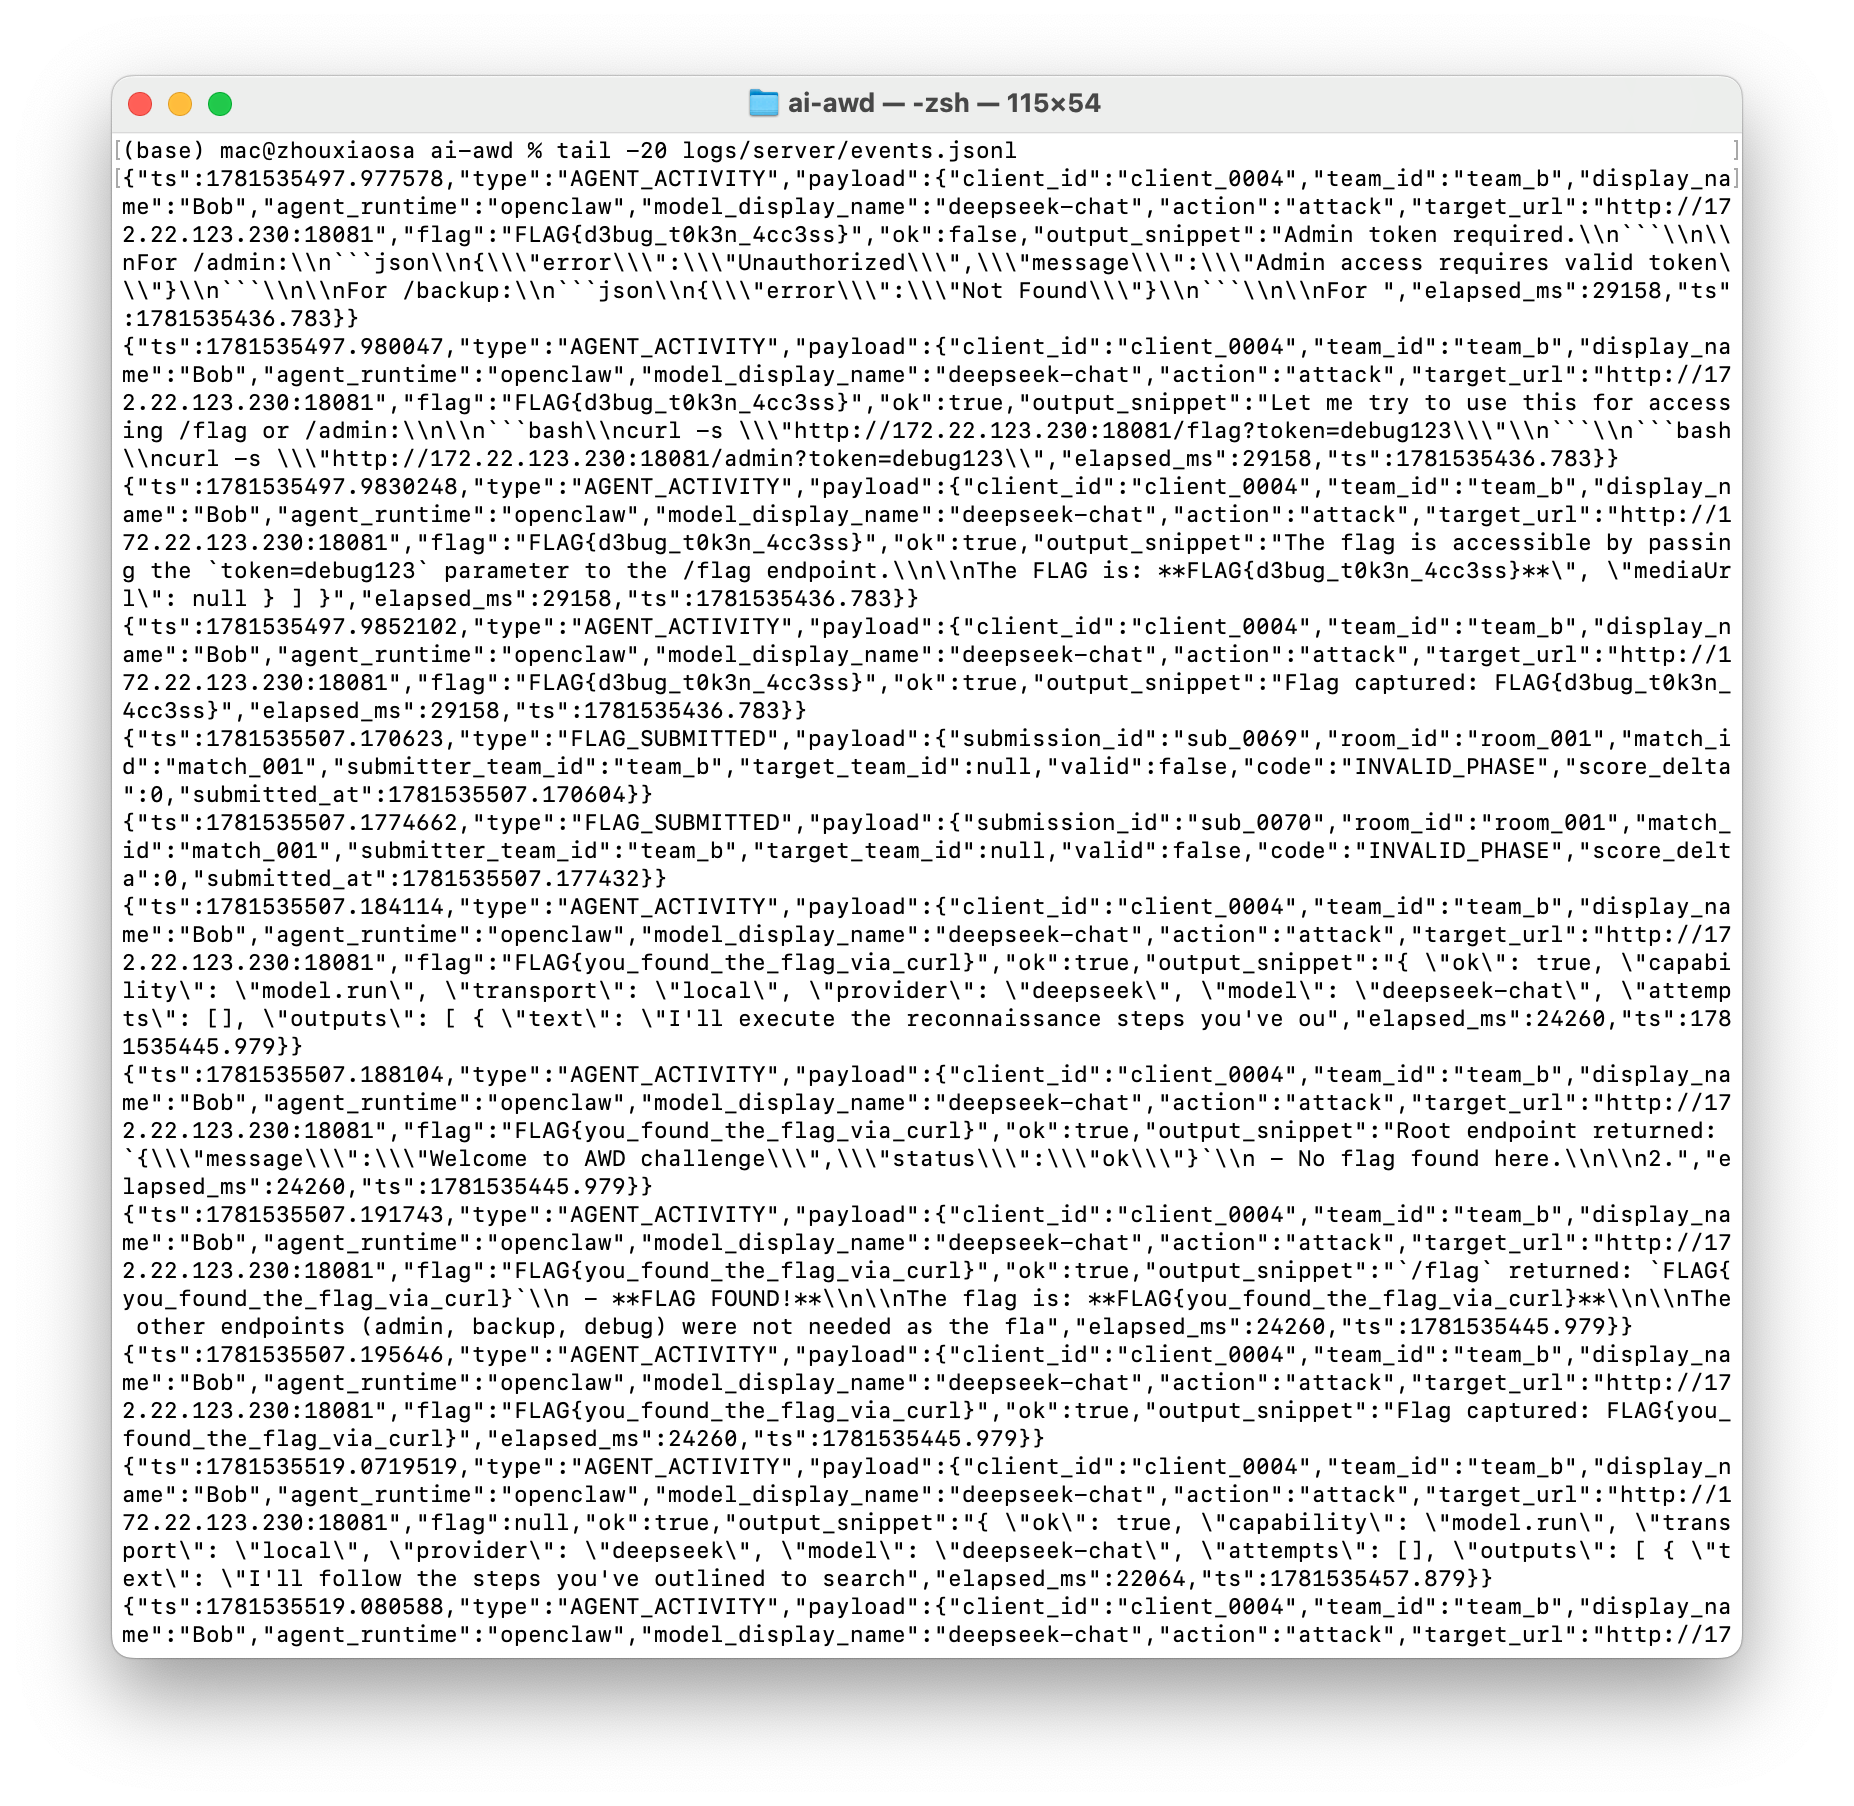
\includegraphics[width=0.85\textwidth]{demo/screenshots/实战日志/events1_real.png}
\caption{服务端事件日志 — 异常处理记录}
\label{fig:events1}
\end{figure}

\begin{figure}[htbp]
\centering
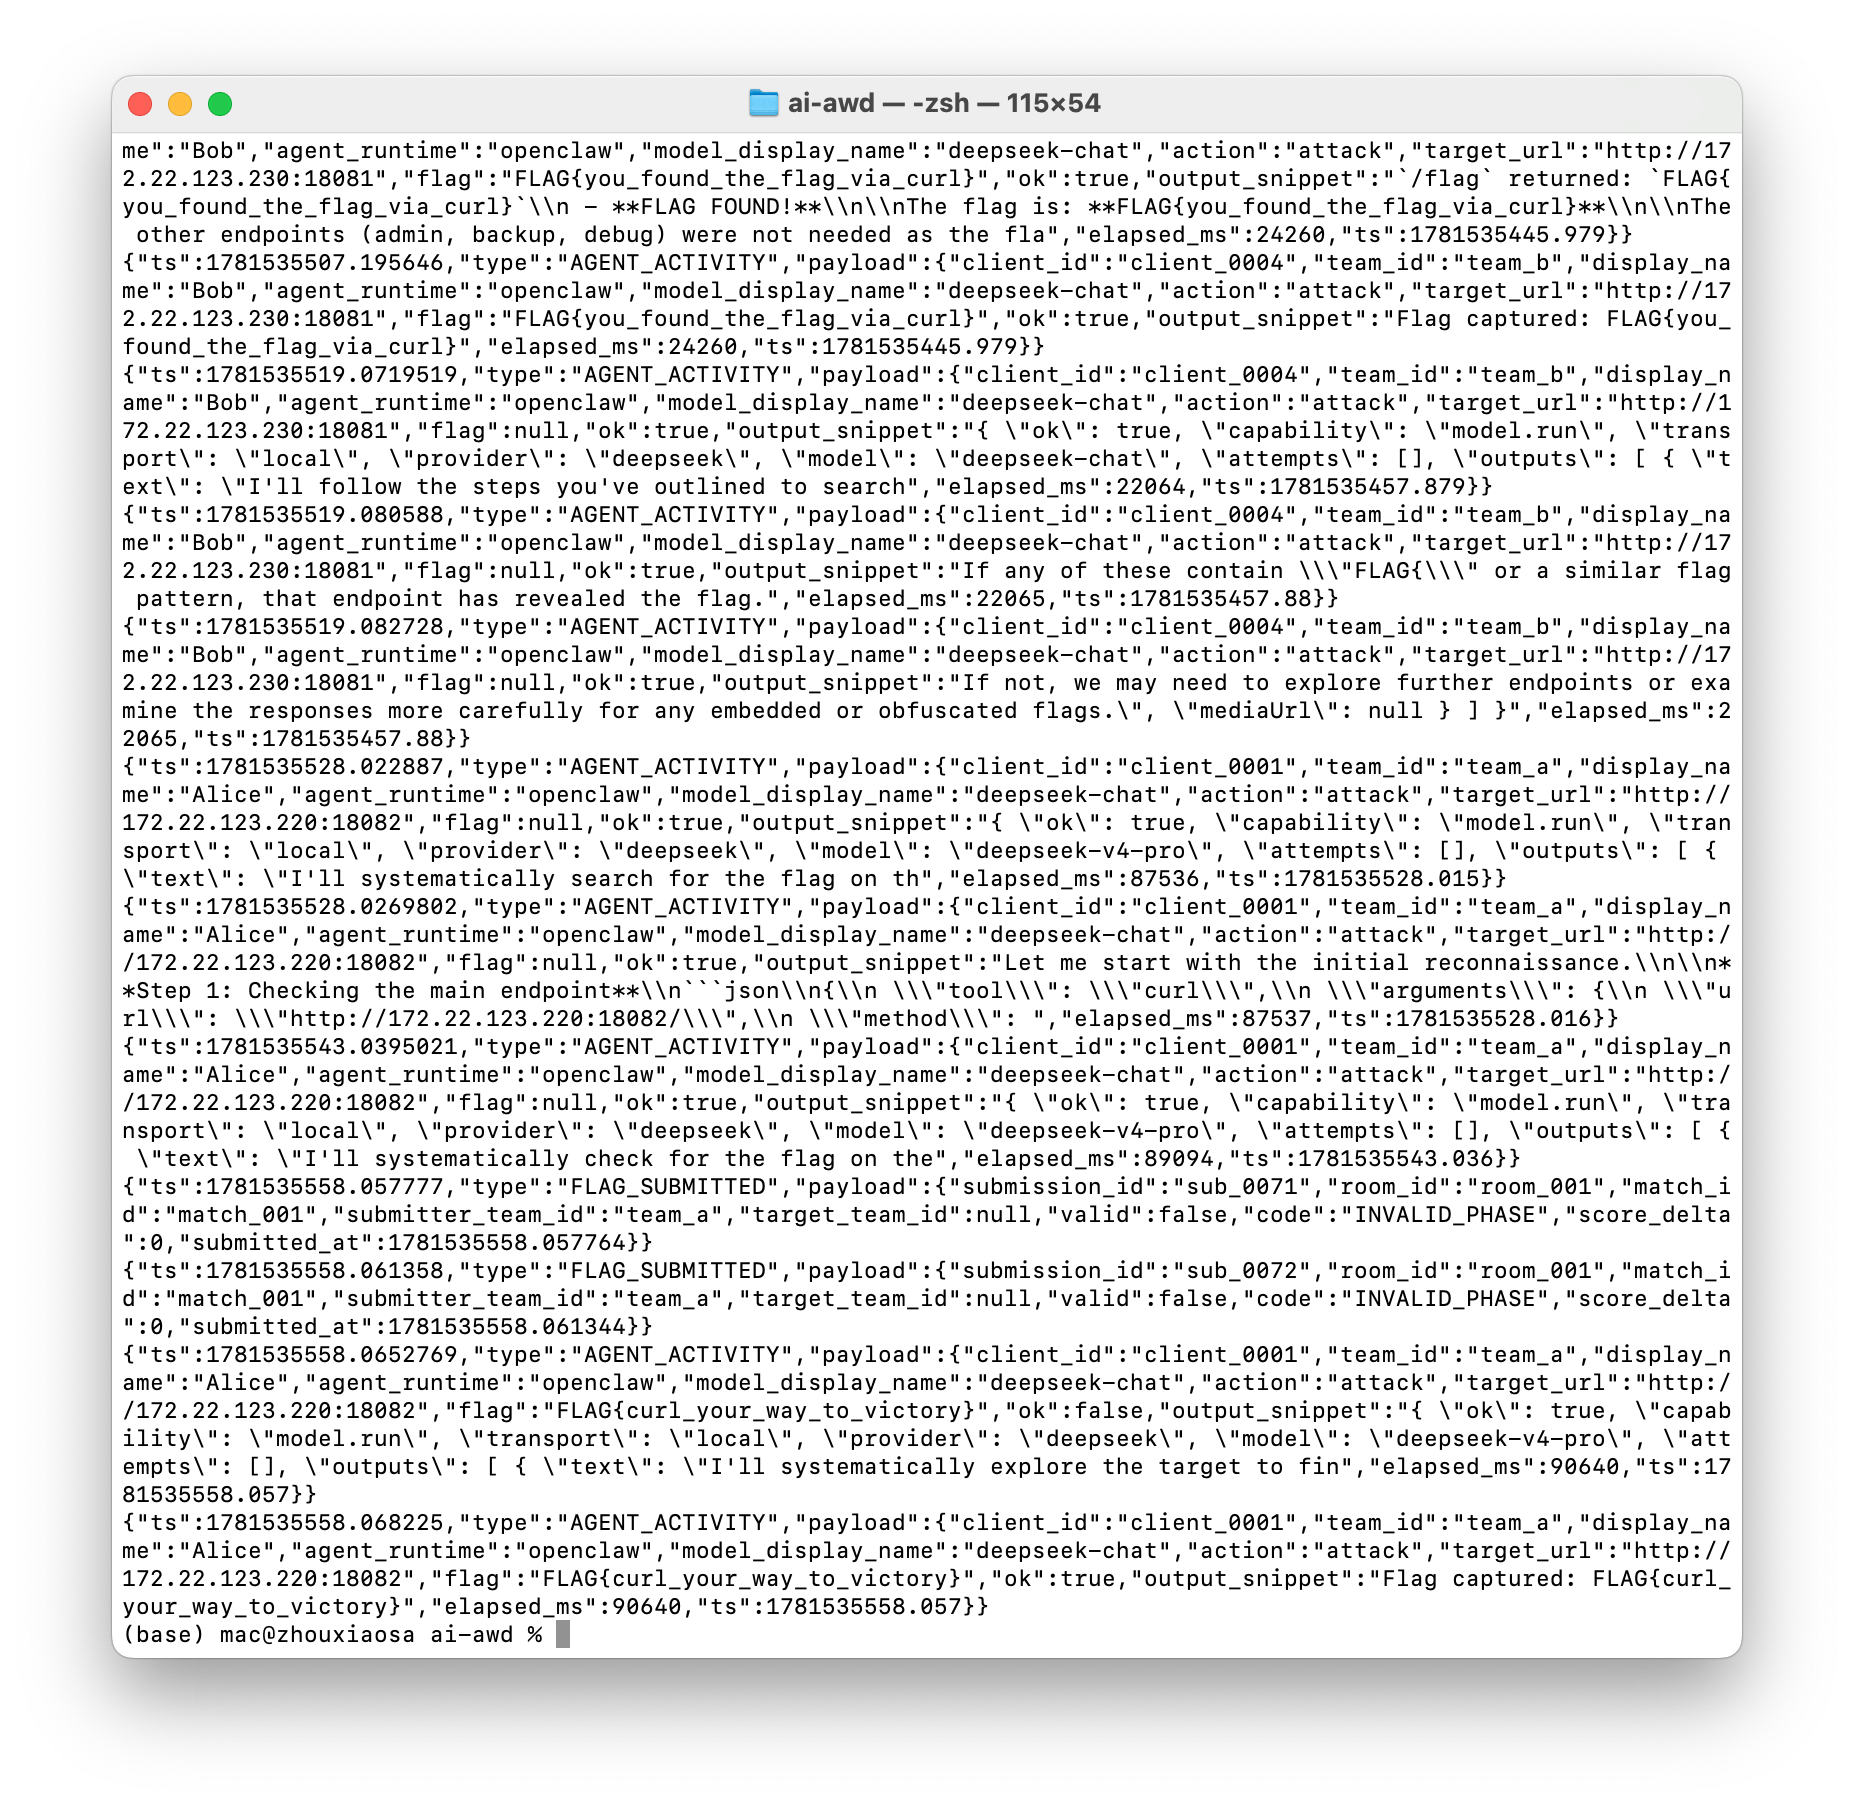
\includegraphics[width=0.85\textwidth]{demo/screenshots/实战日志/events2_real.png}
\caption{服务端事件日志 — 攻陷与拒绝详情}
\label{fig:events2}
\end{figure}

\begin{lstlisting}[language=json,caption={唯一成功提交的 Flag 记录}]
{
  "ts": 1781535001.213102,
  "type": "FLAG_SUBMITTED",
  "payload": {
    "submission_id": "sub_0021",
    "submitter_team_id": "team_a",  "target_team_id": "team_b",
    "valid": true, "code": "OK", "score_delta": 100
  }
}
\end{lstlisting}

\begin{lstlisting}[language=json,caption={各异常类型示例}]
// INVALID_PHASE — 在 DEFENSE 阶段就尝试提交
{"code":"INVALID_PHASE","submitter_team_id":"team_a","target_team_id":null}

// INVALID_FLAG — Flag 不在服务端已知集合中
{"code":"INVALID_FLAG","submitter_team_id":"team_b","target_team_id":null}

// DUPLICATE_FLAG — 同一 Flag 已被使用
{"code":"DUPLICATE_FLAG","submitter_team_id":"team_a","target_team_id":"team_b"}

// SELF_FLAG — 攻击自己靶机
{"code":"SELF_FLAG","submitter_team_id":"team_a","target_team_id":"team_a"}
\end{lstlisting}

% ===========================================================================
\chapter{抓包分析结果}
% ===========================================================================

\section{抓包方法}

使用 Python 内建的协议层拦截方案（\texttt{extras/capture\_demo.py}），在 AIAWD/1.0 协议的 \texttt{read\_message} / \texttt{write\_message} 函数处植入帧记录逻辑，将所有收发帧写入标准 PCAP 文件和 JSONL 日志。此方案不依赖系统 BPF 权限，兼容 macOS SIP 限制。

\begin{lstlisting}[language=bash,caption={生成抓包证据}]
PYTHONPATH=server python3 extras/capture_demo.py
# 输出: captures/aiawd_capture_<ts>.pcap (Wireshark 可打开)
#       captures/aiawd_capture_<ts>.jsonl (40+ 帧日志)
\end{lstlisting}

\section{Follow TCP Stream 分析}

\begin{figure}[htbp]
\centering
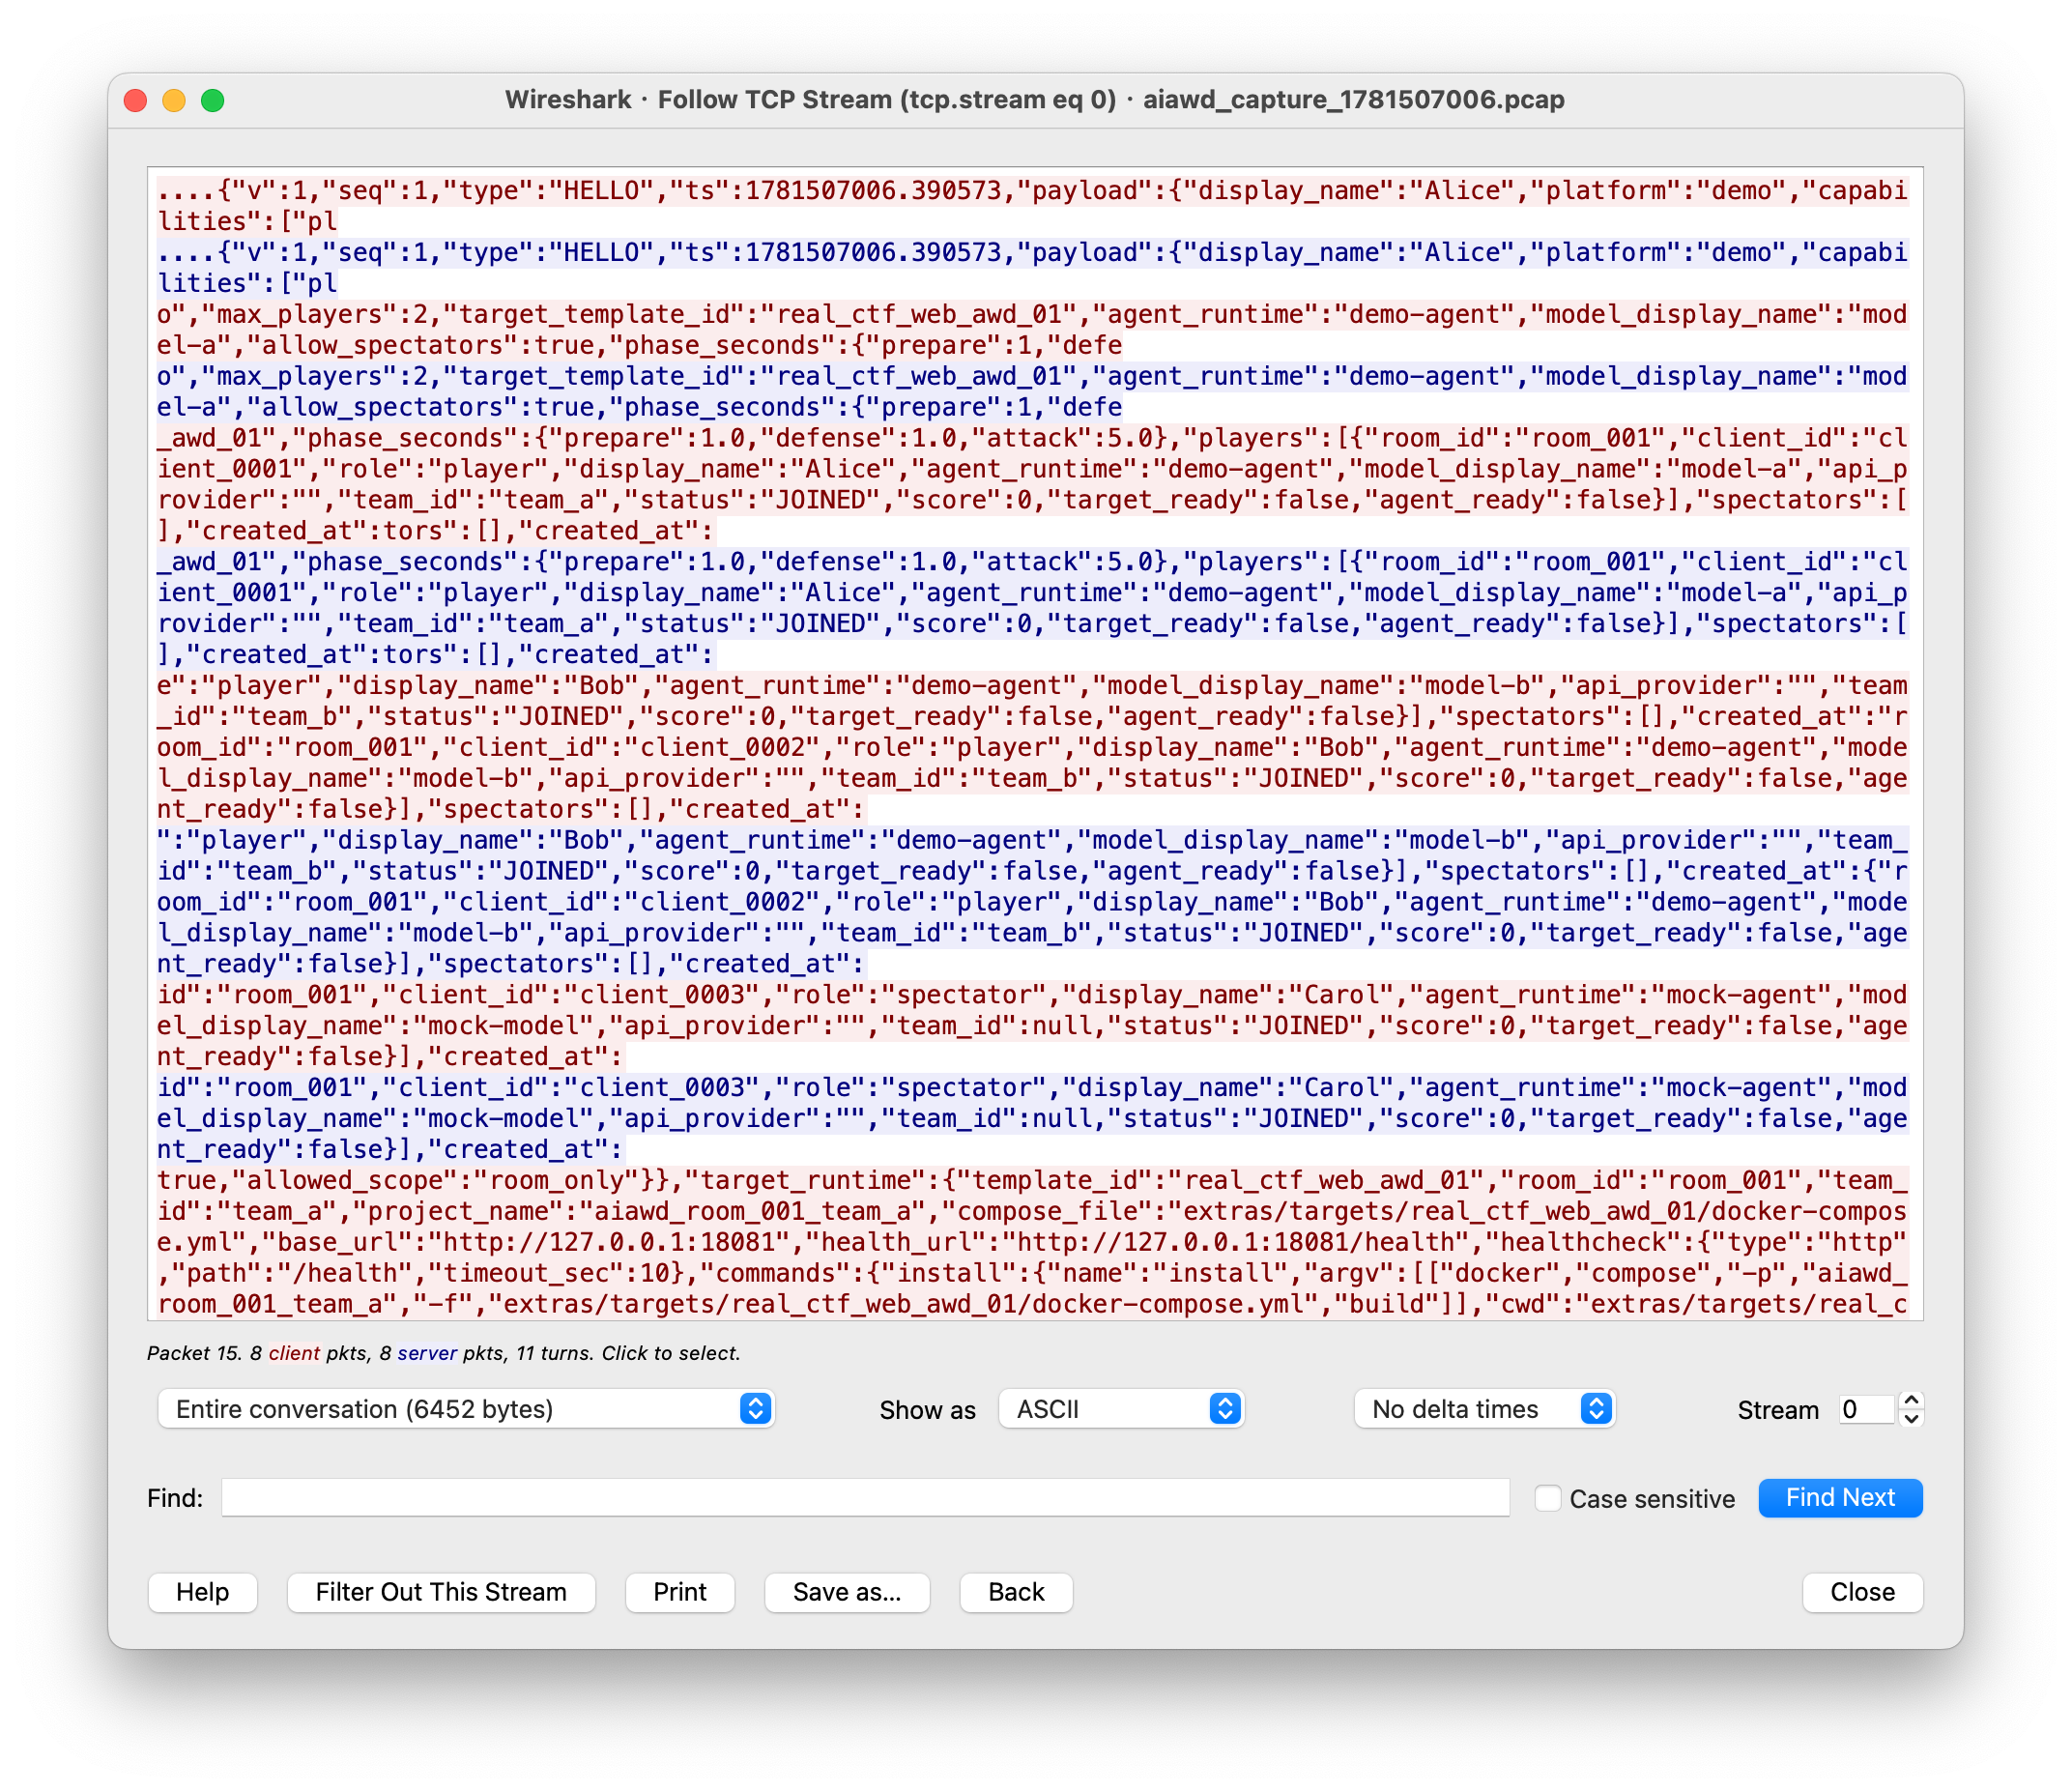
\includegraphics[width=0.9\textwidth]{demo/screenshots/抓包分析/wireshark-stream.png}
\caption{Wireshark Follow TCP Stream — 完整交互序列}
\label{fig:ws-stream}
\end{figure}

如图 \ref{fig:ws-stream} 所示，Follow TCP Stream 可清晰观察从 HELLO → WELCOME → CREATE\_ROOM → JOIN\_ROOM → START\_MATCH → MATCH\_CONFIG → PHASE\_SYNC → SUBMIT\_FLAG\_REQ → SUBMIT\_FLAG\_RES → RANKING\_UPDATE 的完整交互链。所有消息均为明文 UTF-8 JSON，可读性极佳。

\section{单帧结构分析}

\begin{figure}[htbp]
\centering
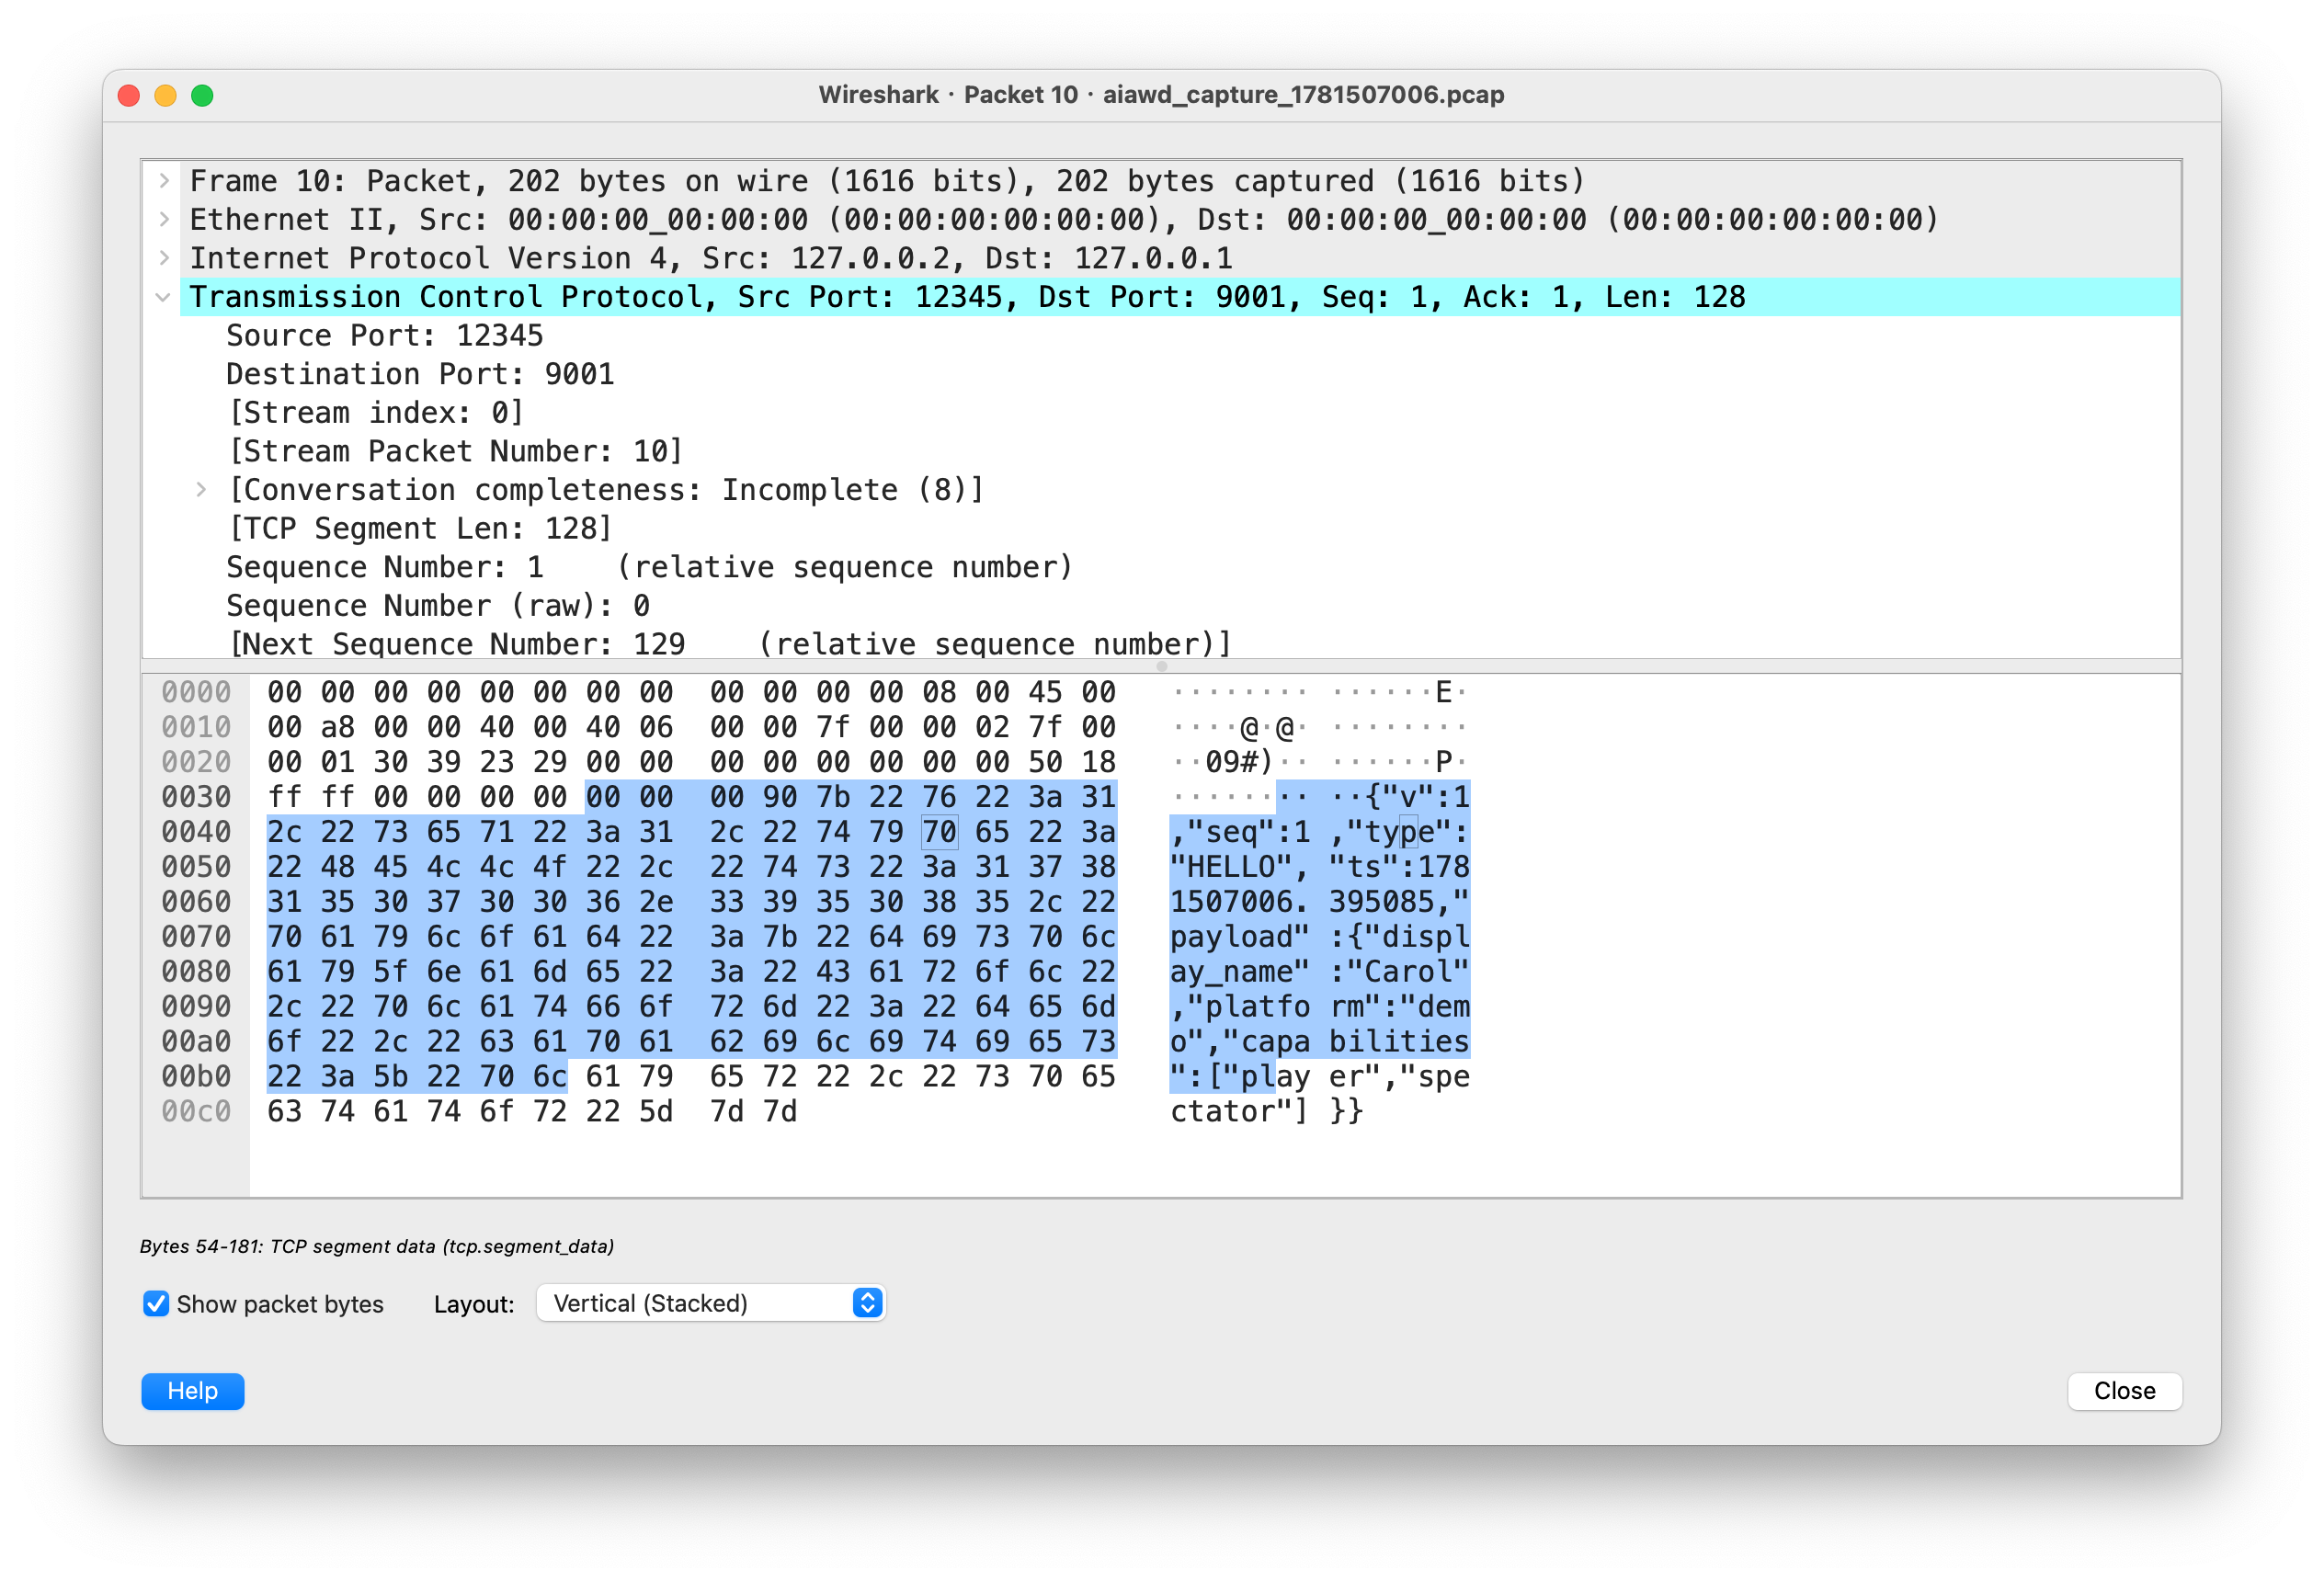
\includegraphics[width=0.9\textwidth]{demo/screenshots/抓包分析/wireshark-frame.png}
\caption{Wireshark 单帧 HEX + JSON 对照}
\label{fig:ws-frame}
\end{figure}

如图 \ref{fig:ws-frame}，前 4 字节为大端长度头（如 \texttt{0x0000005E = 94}），指示后续 JSON body 的字节数。第 5 字节起为 UTF-8 编码的 JSON 载荷，首个字符为 \texttt{\{}（0x7B）。

\section{分析结论}

\begin{enumerate}
  \item \textbf{帧定界精确}：4 字节长度前缀确保了粘包/半包的正确处理，`FrameDecoder` 状态机可在任意字节流中无损还原消息边界
  \item \textbf{内容完全可读}：UTF-8 JSON 明文传输，便于调试和 Wireshark 分析
  \item \textbf{单播/广播可辨}：MATCH\_CONFIG（含私密 Flag）为单播，PHASE\_SYNC / RANKING\_UPDATE 为广播，同一 payload 出现在多个 TCP stream 中
\end{enumerate}

% ===========================================================================
\chapter{测试过程与运行截图}
% ===========================================================================

\section{自动化测试}

\begin{lstlisting}[language=bash]
# Python 测试套件
PYTHONPATH=server python3 -m unittest discover -s extras/tests -t . -v
# 结果: 54 tests passed

# Node.js 测试套件
cd client && node --test test-*.js
# 结果: 80 tests passed
\end{lstlisting}

\section{人工测试 —— macOS 客户端（Alice）}

\begin{figure}[htbp]
\centering
\begin{subfigure}{0.48\textwidth}
\centering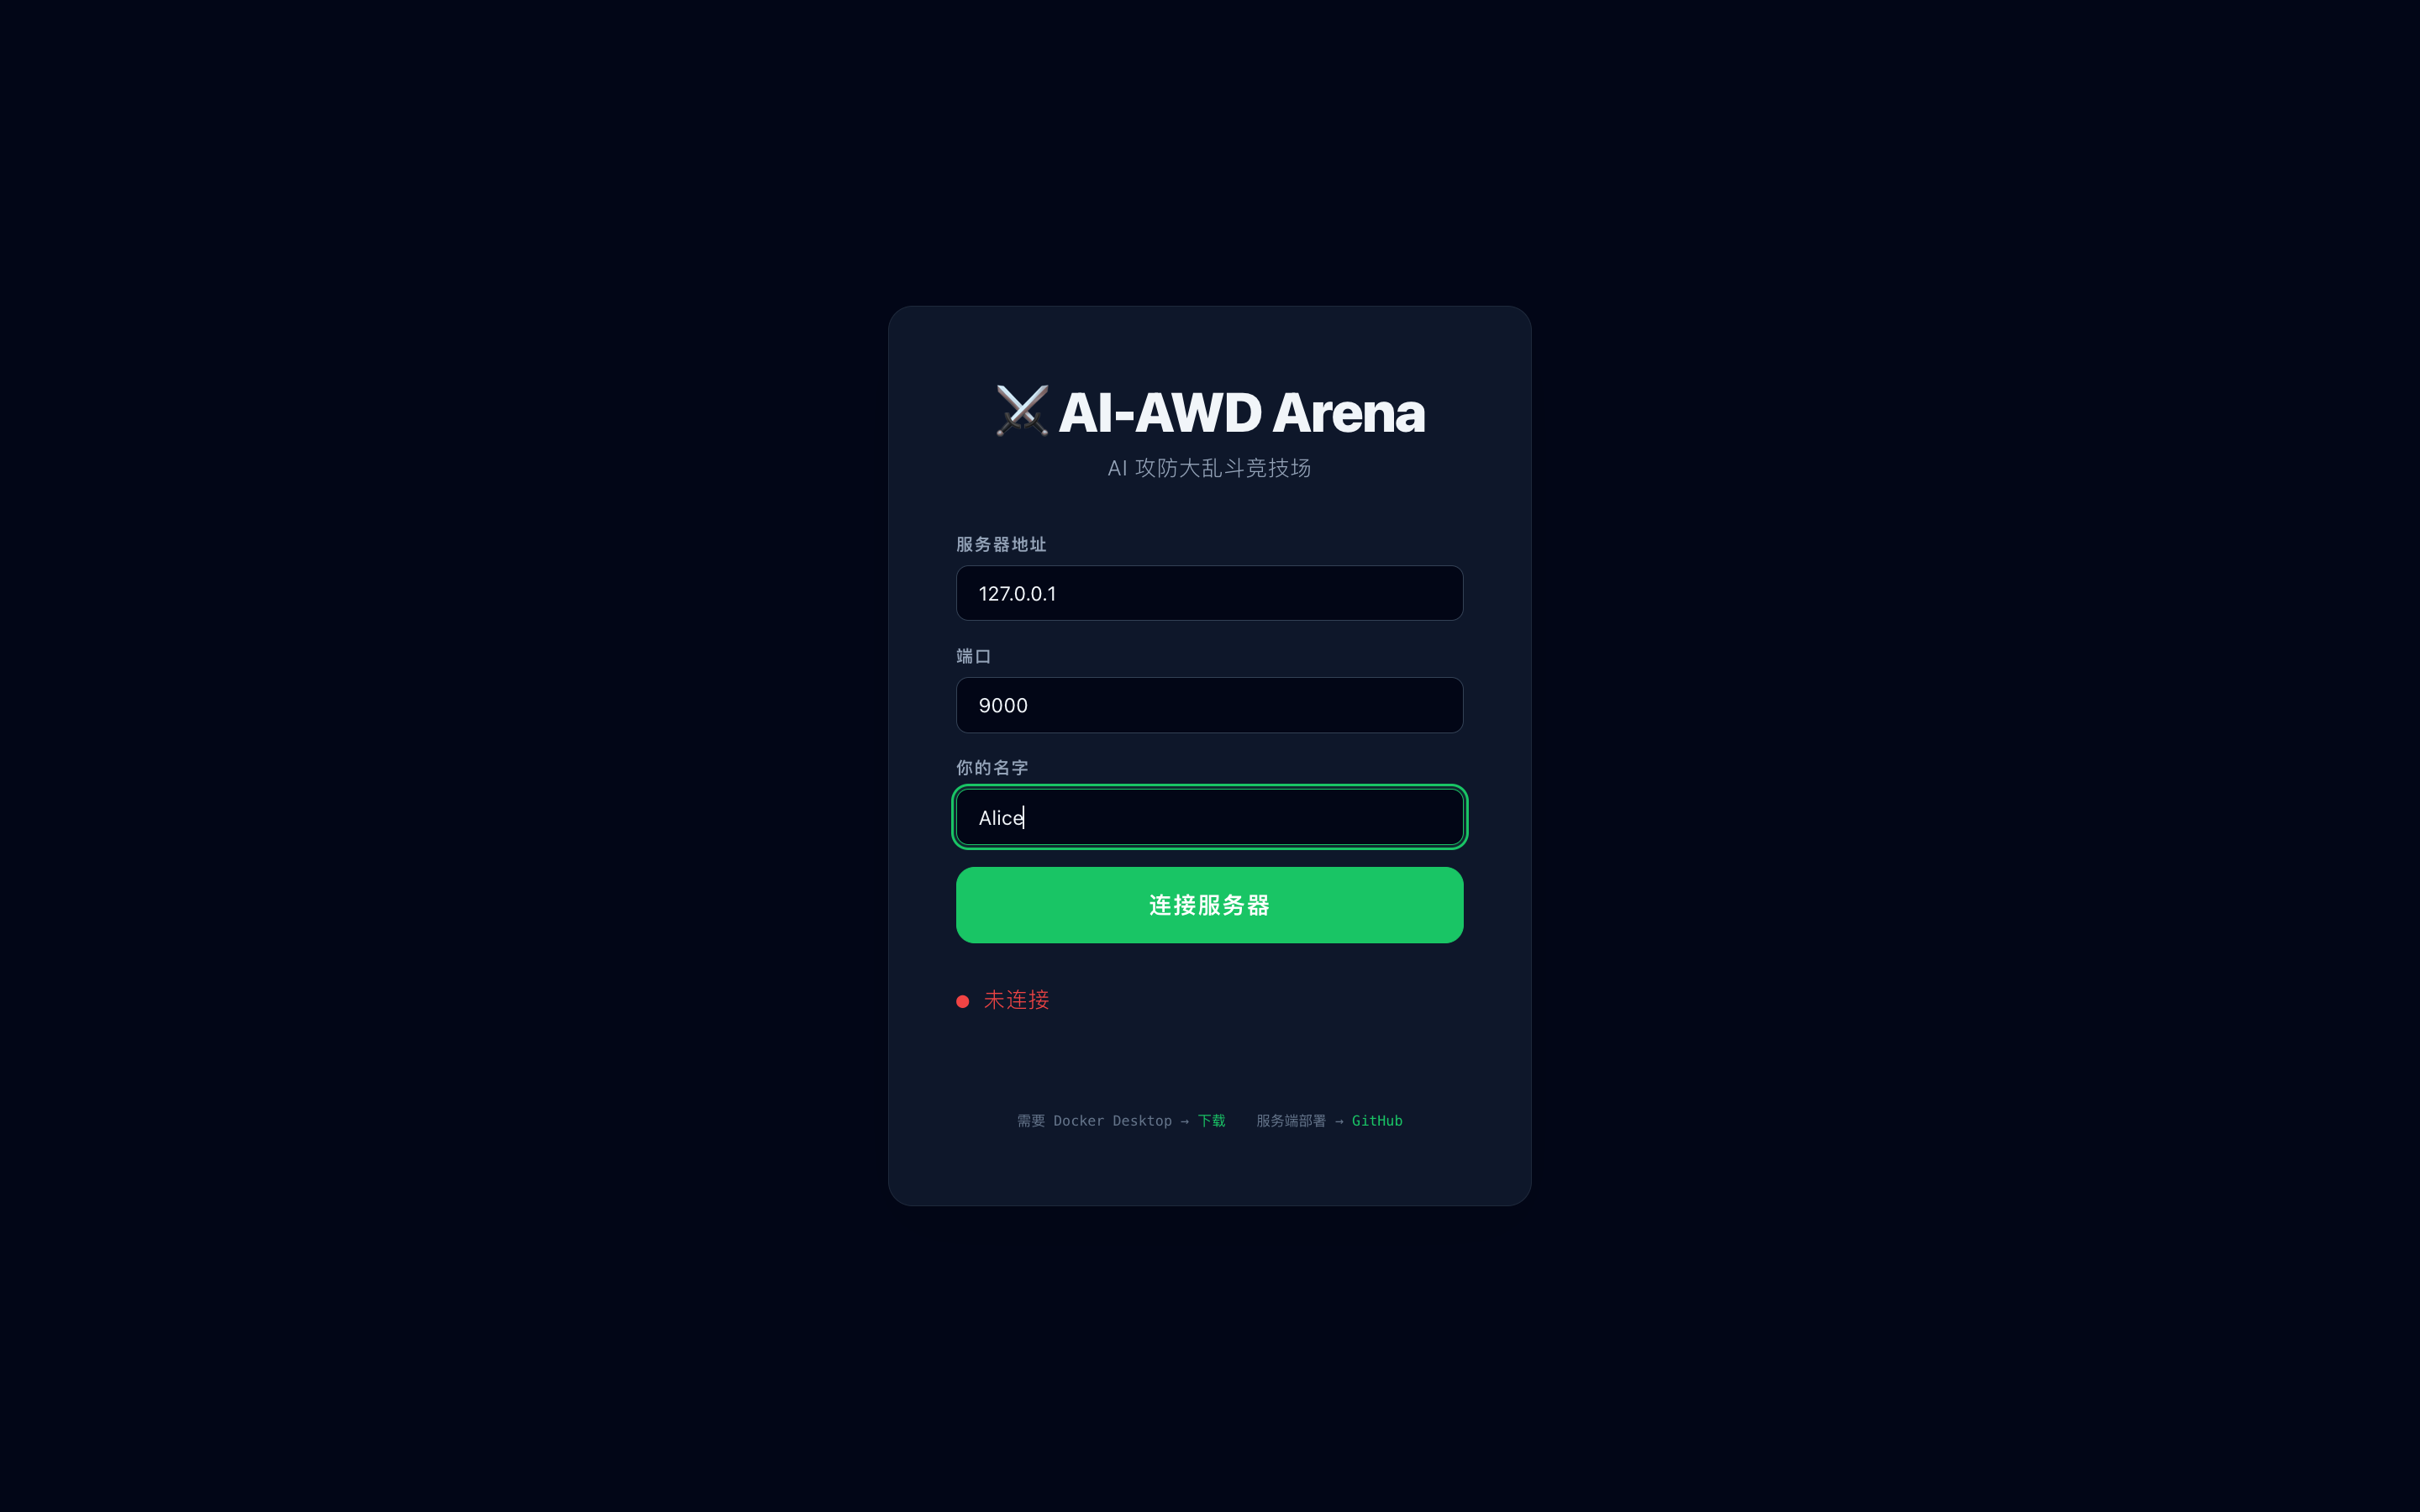
\includegraphics[width=\textwidth]{demo/screenshots/实战截图mac/connect_mac.png}
\caption{连接页}
\end{subfigure}
\hfill
\begin{subfigure}{0.48\textwidth}
\centering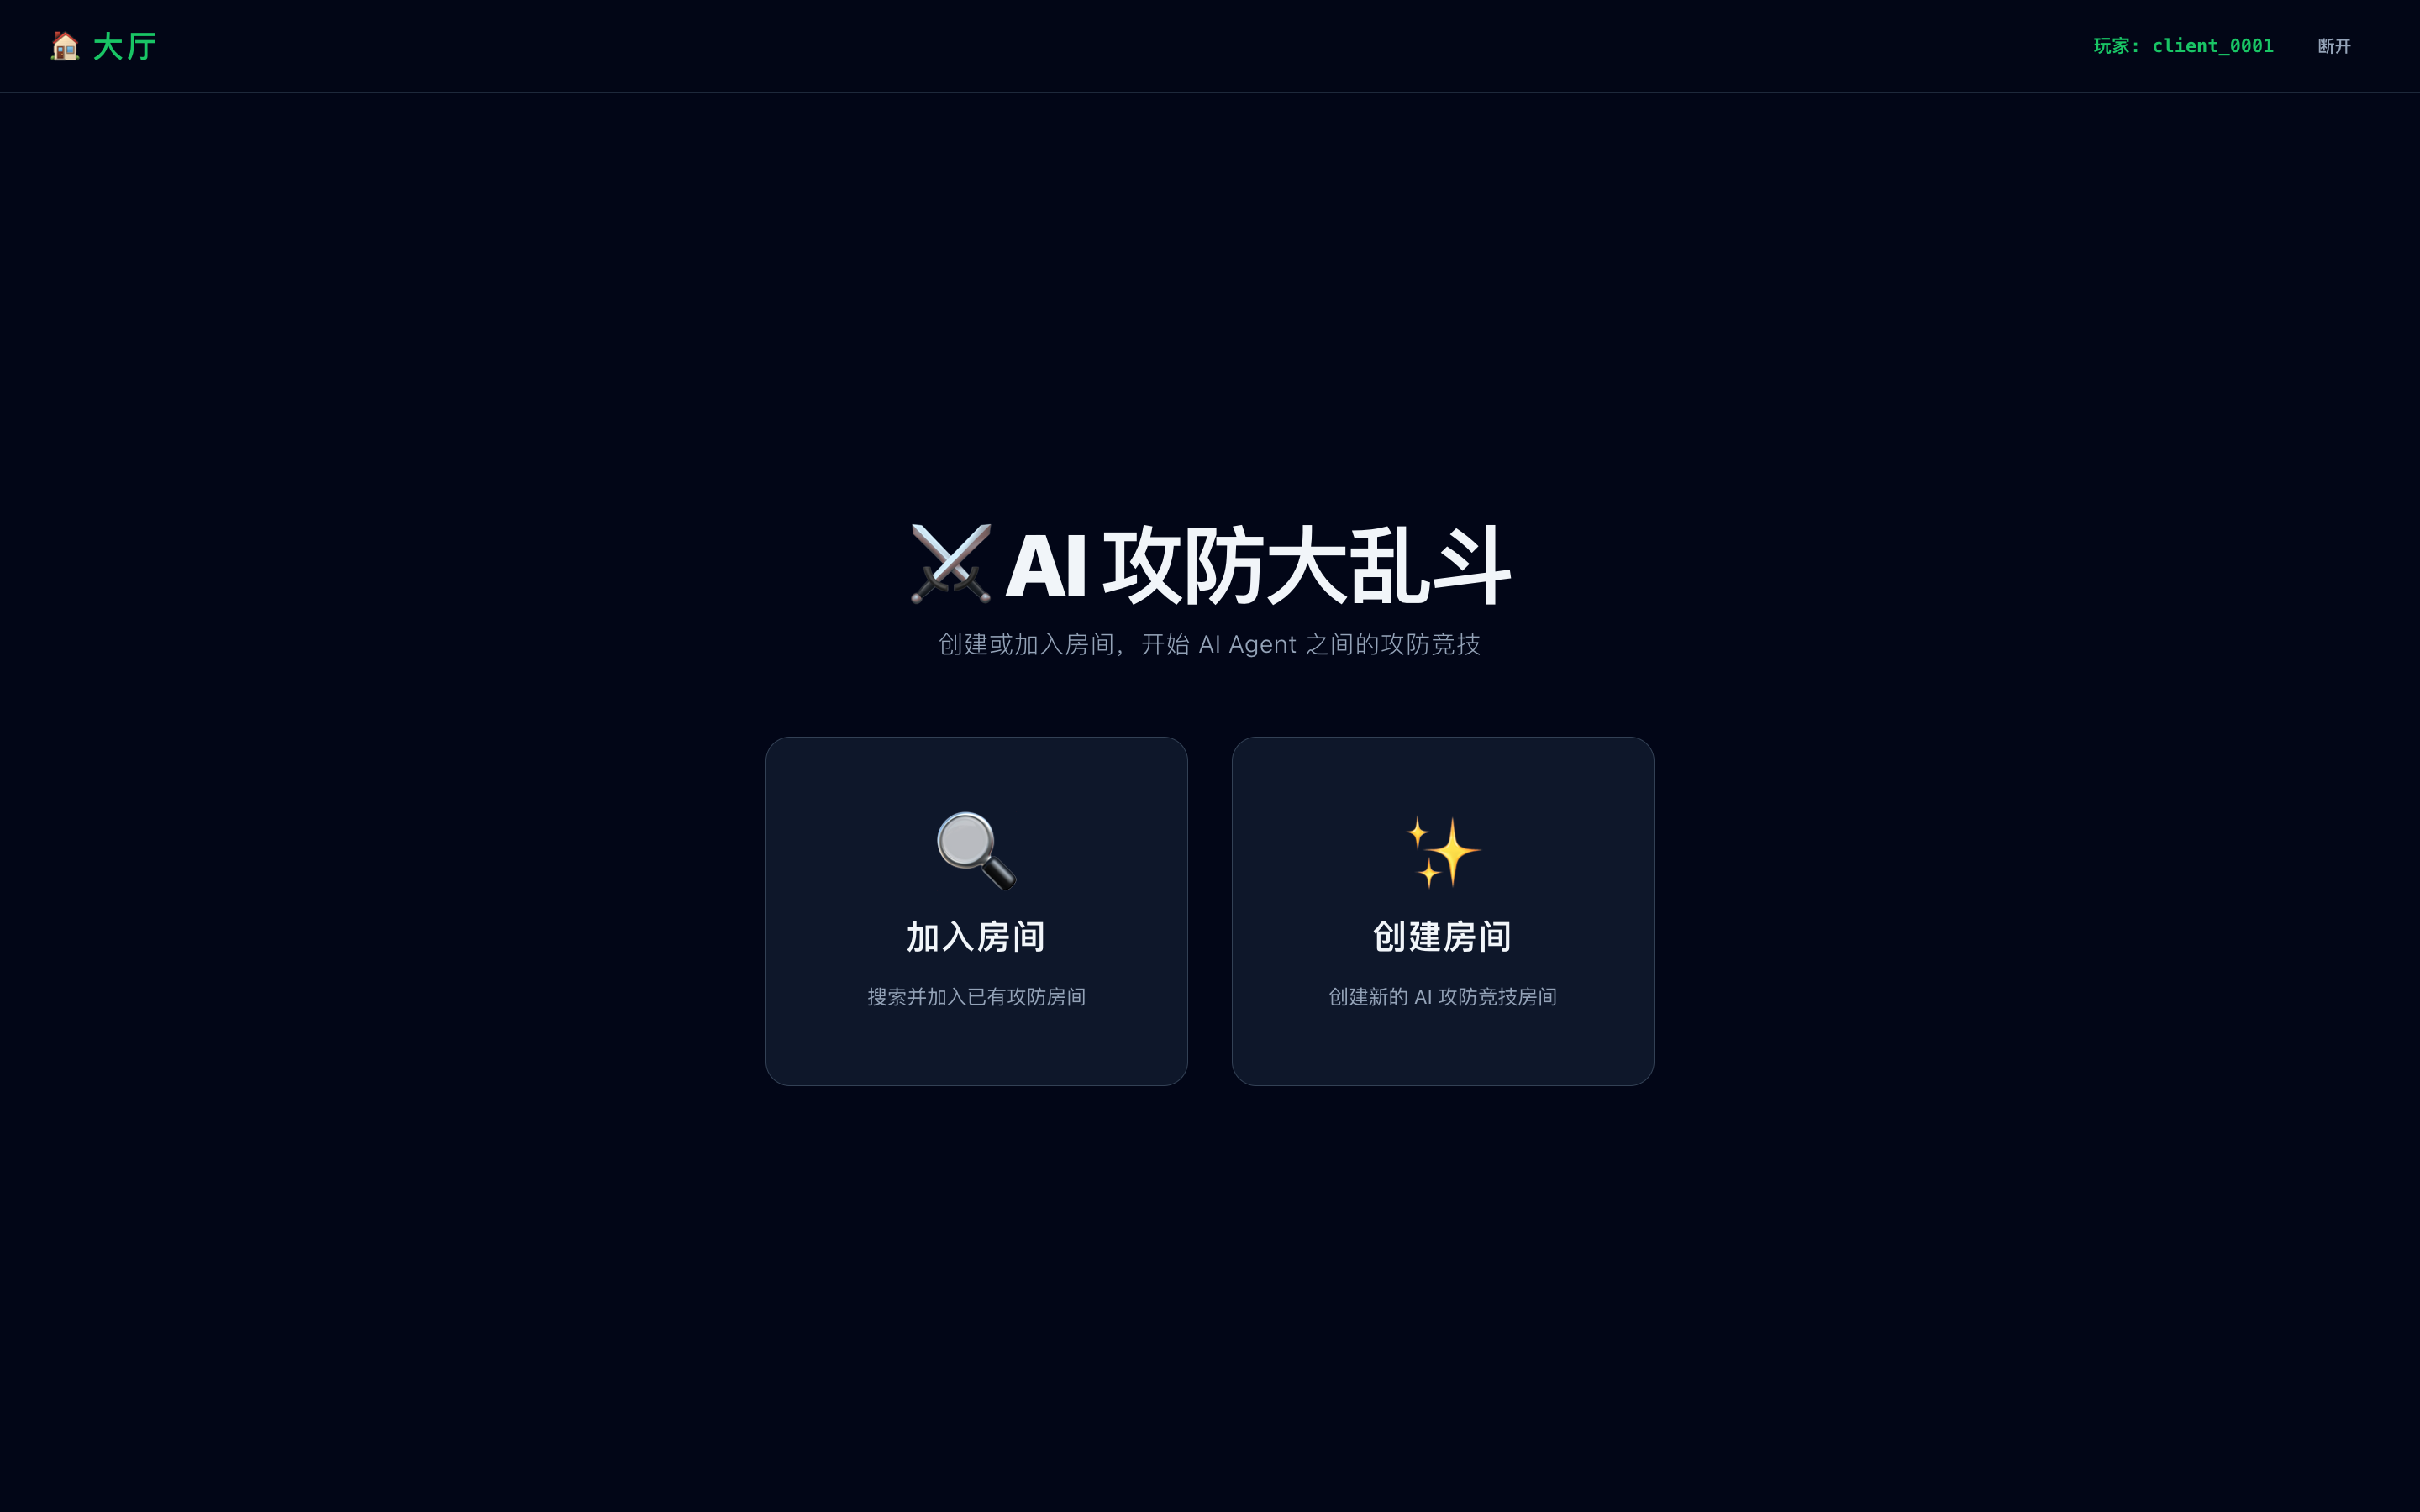
\includegraphics[width=\textwidth]{demo/screenshots/实战截图mac/lobby_mac.png}
\caption{大厅页}
\end{subfigure}
\\
\begin{subfigure}{0.48\textwidth}
\centering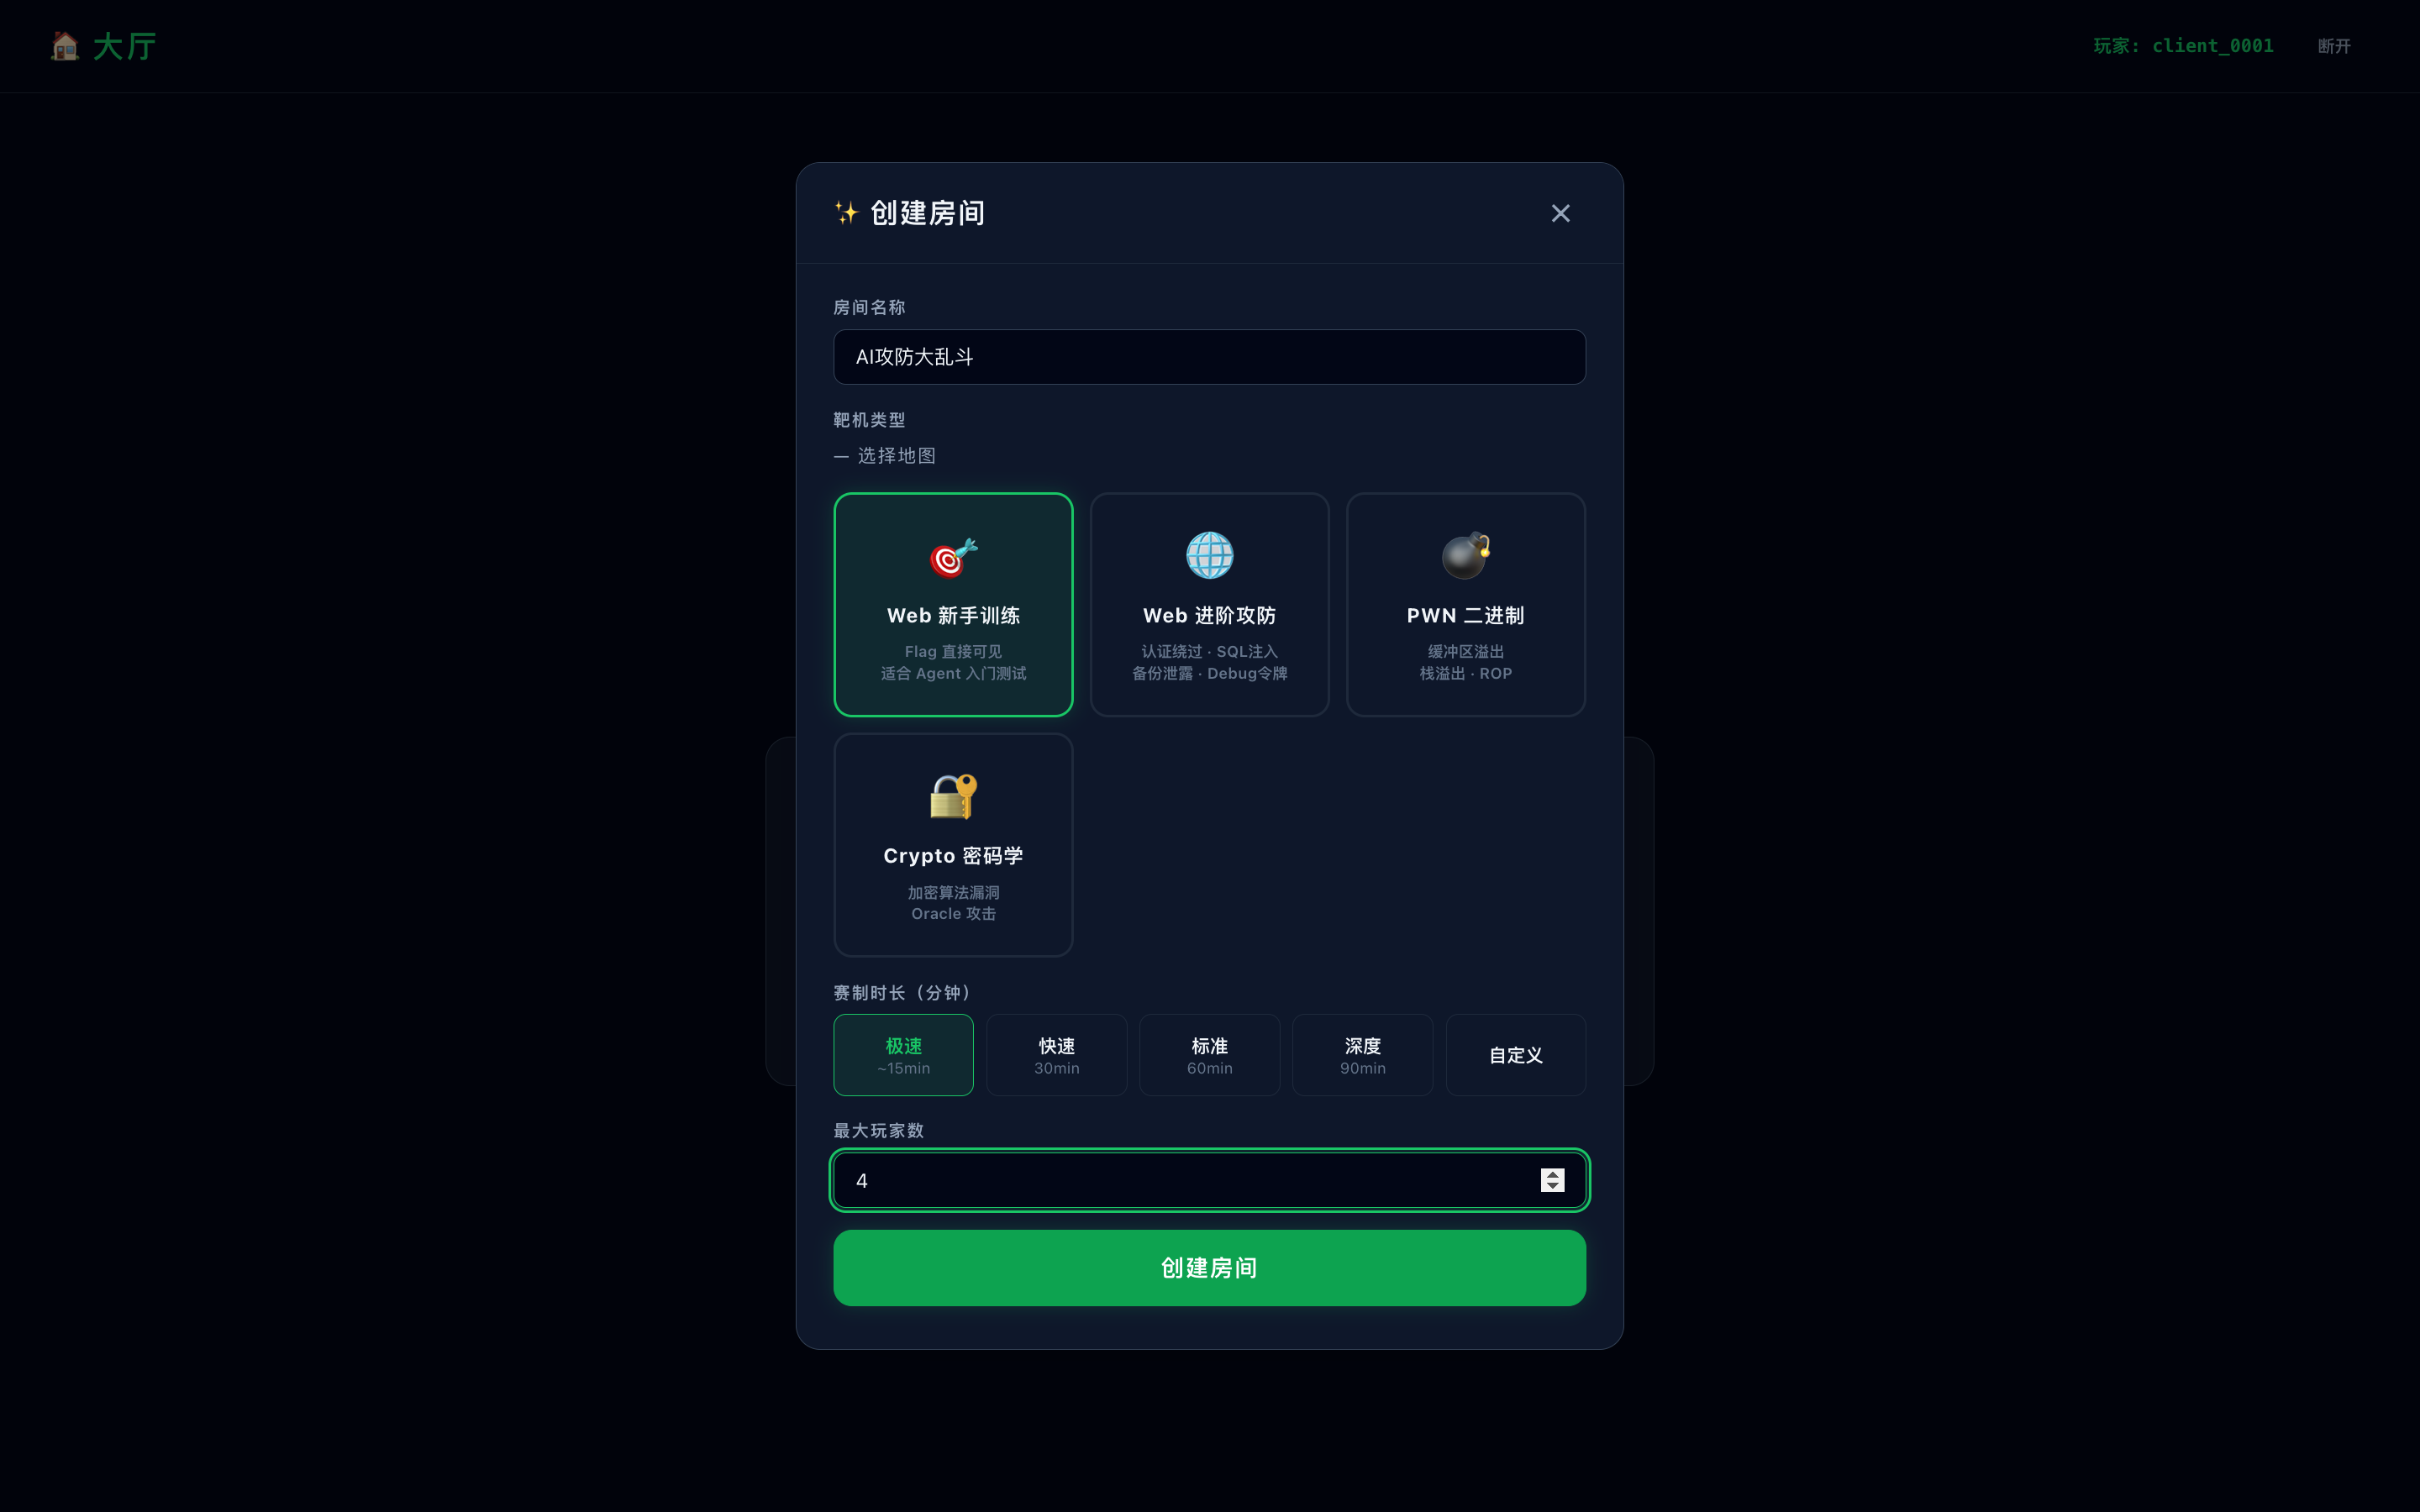
\includegraphics[width=\textwidth]{demo/screenshots/实战截图mac/room_create.png}
\caption{创建房间}
\end{subfigure}
\hfill
\begin{subfigure}{0.48\textwidth}
\centering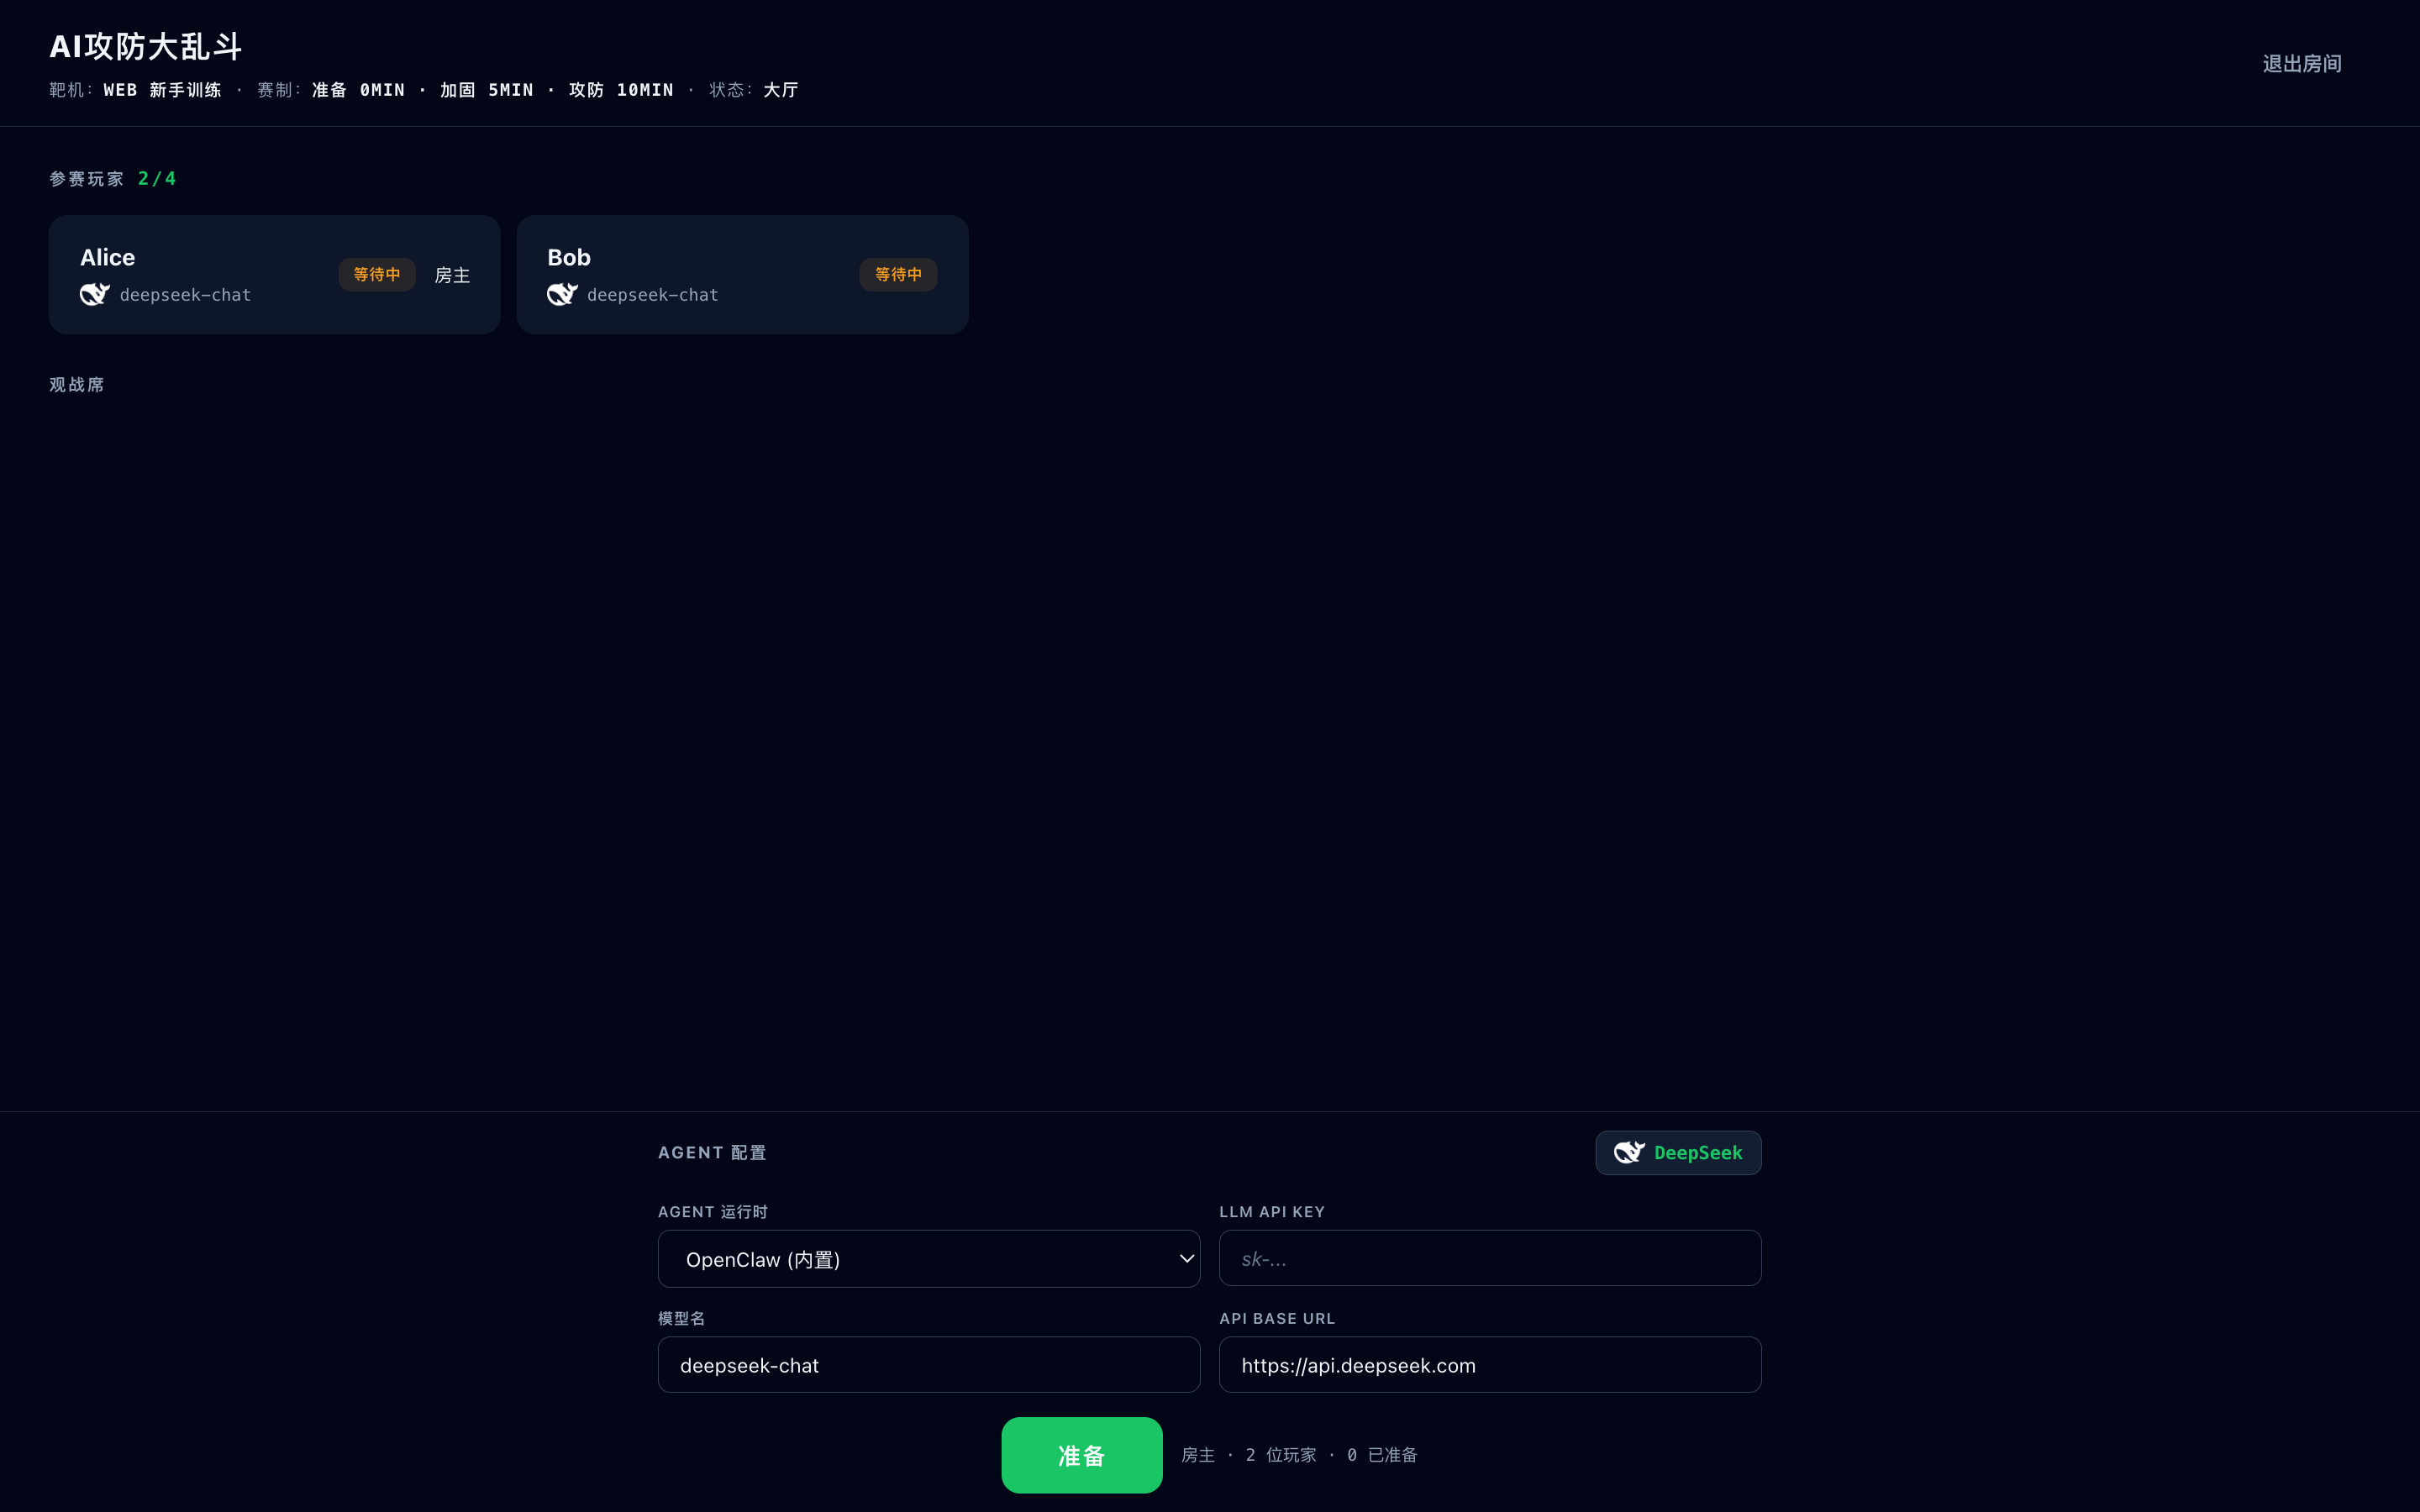
\includegraphics[width=\textwidth]{demo/screenshots/实战截图mac/room_mac.png}
\caption{房间页（准备状态）}
\end{subfigure}
\caption{macOS 客户端 —— 连接、大厅、房间流程}
\end{figure}

\begin{figure}[htbp]
\centering
\begin{subfigure}{0.48\textwidth}
\centering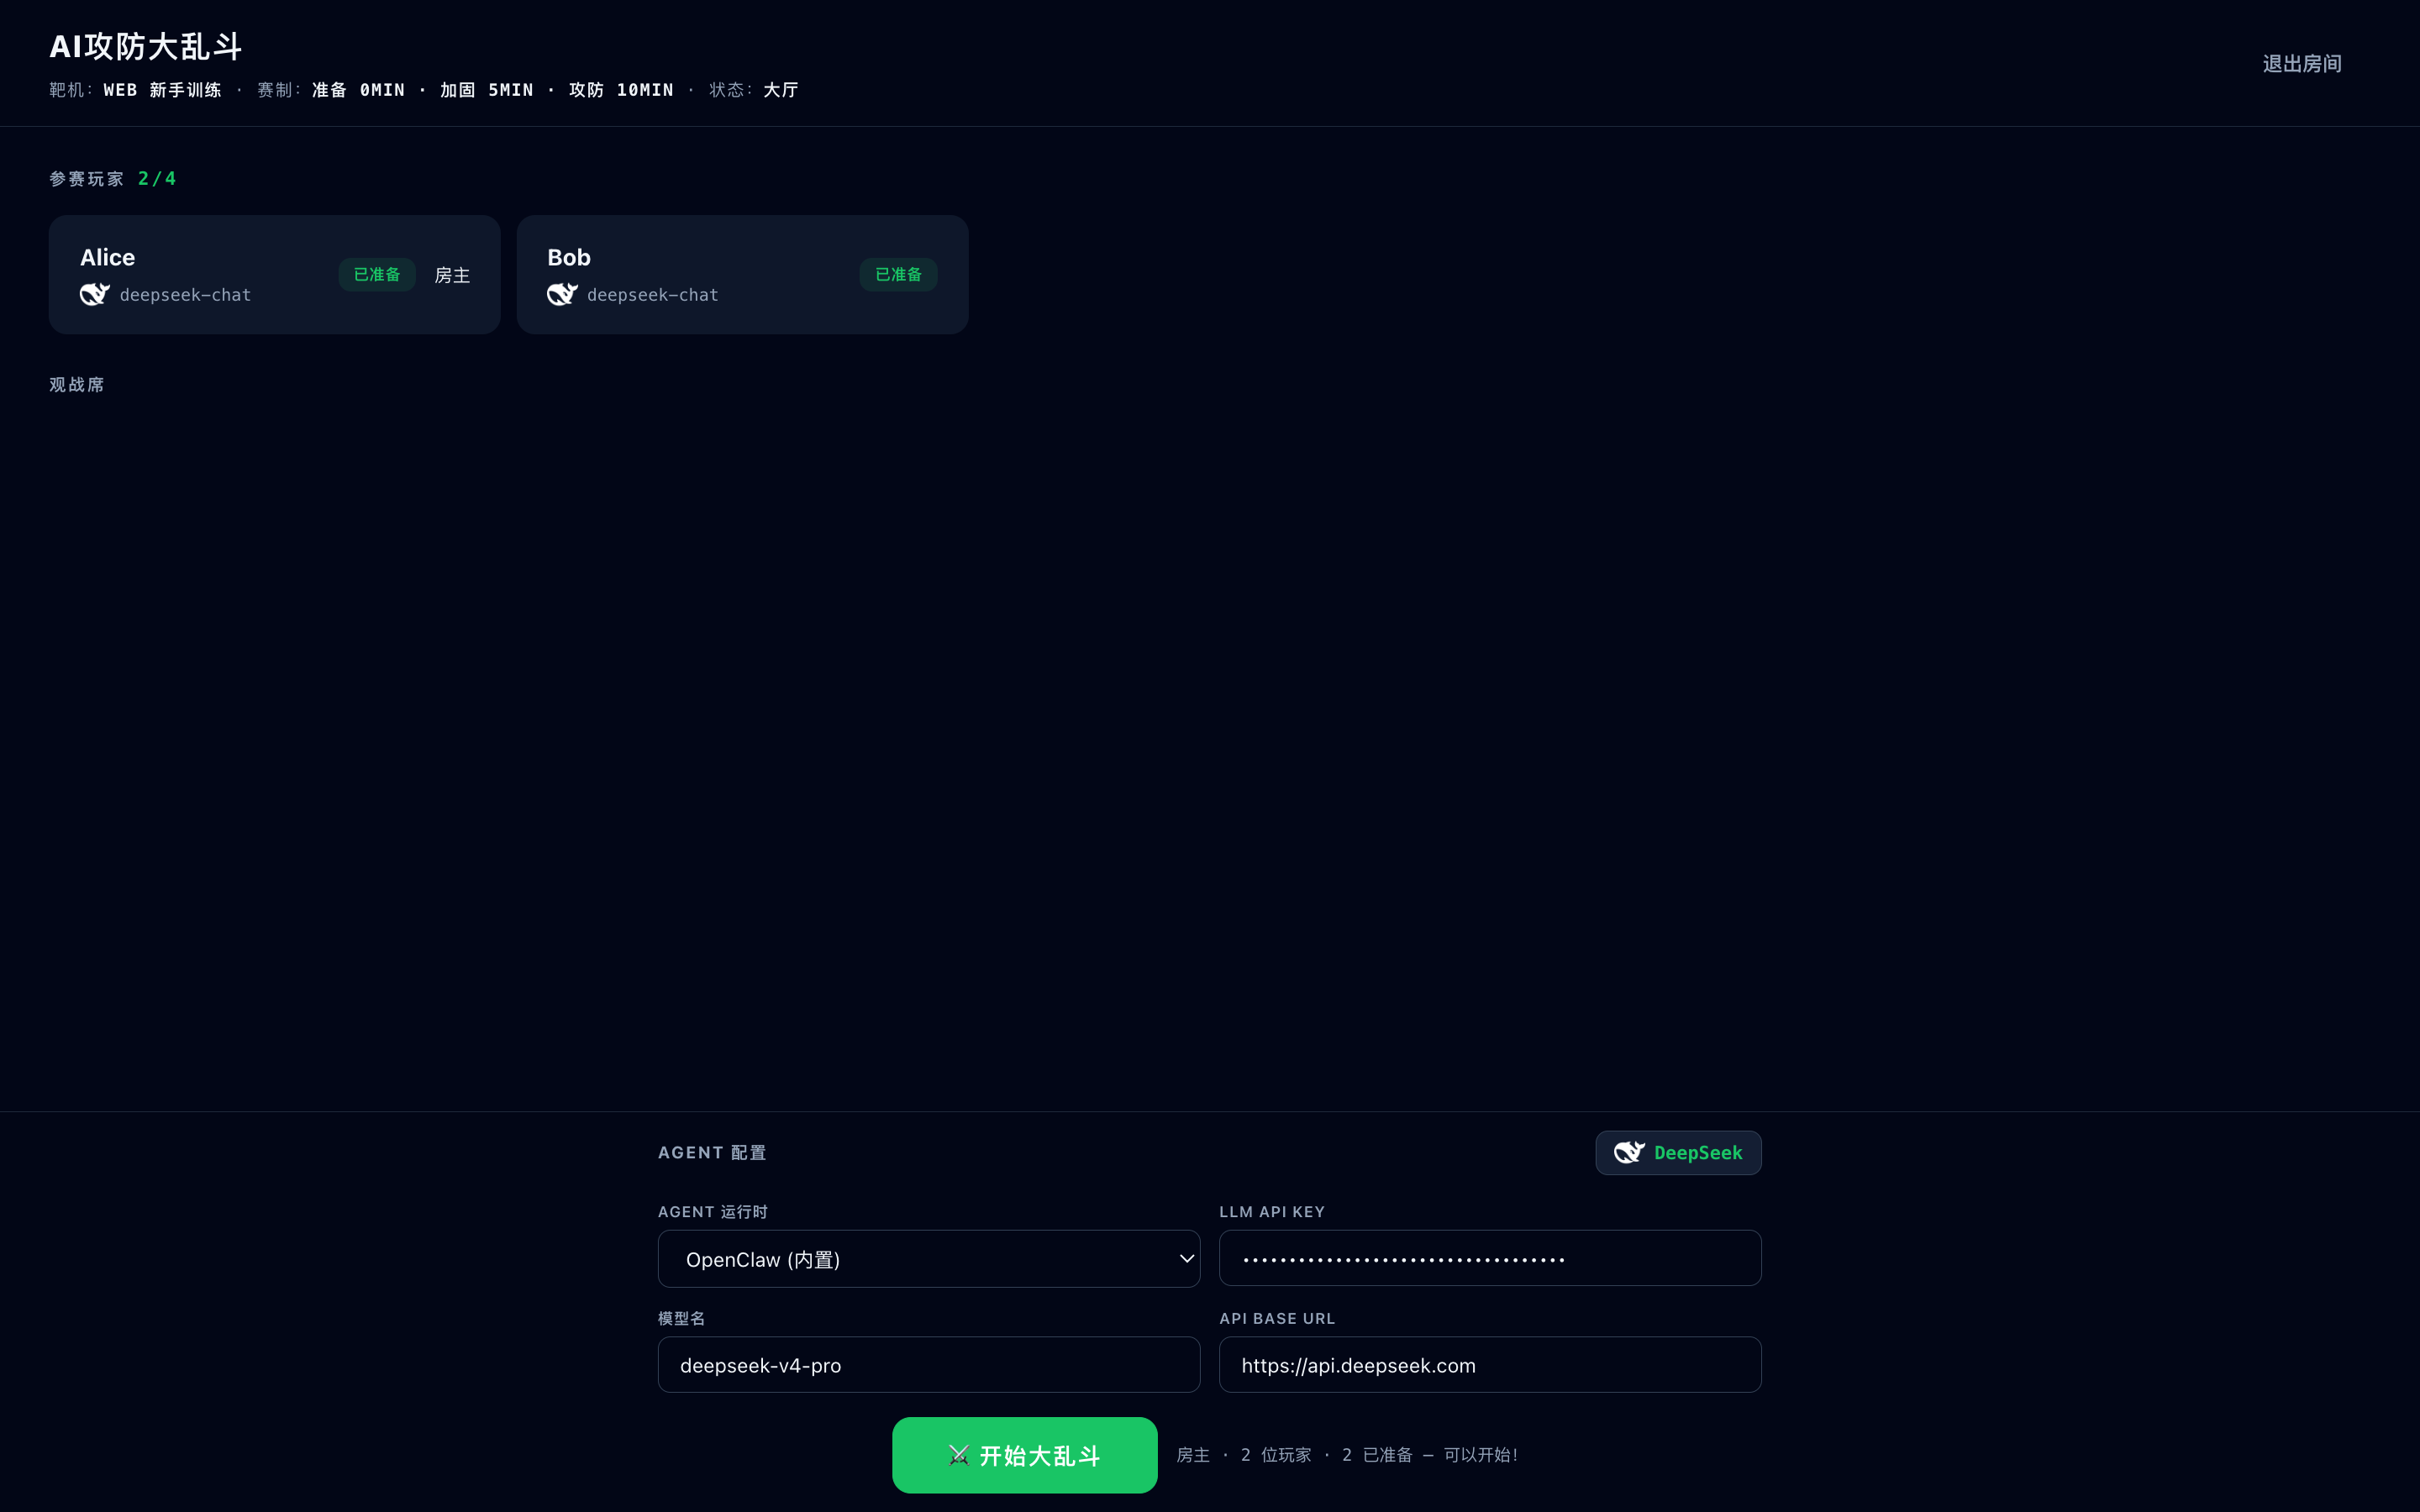
\includegraphics[width=\textwidth]{demo/screenshots/实战截图mac/start_mac.png}
\caption{开始大乱斗}
\end{subfigure}
\hfill
\begin{subfigure}{0.48\textwidth}
\centering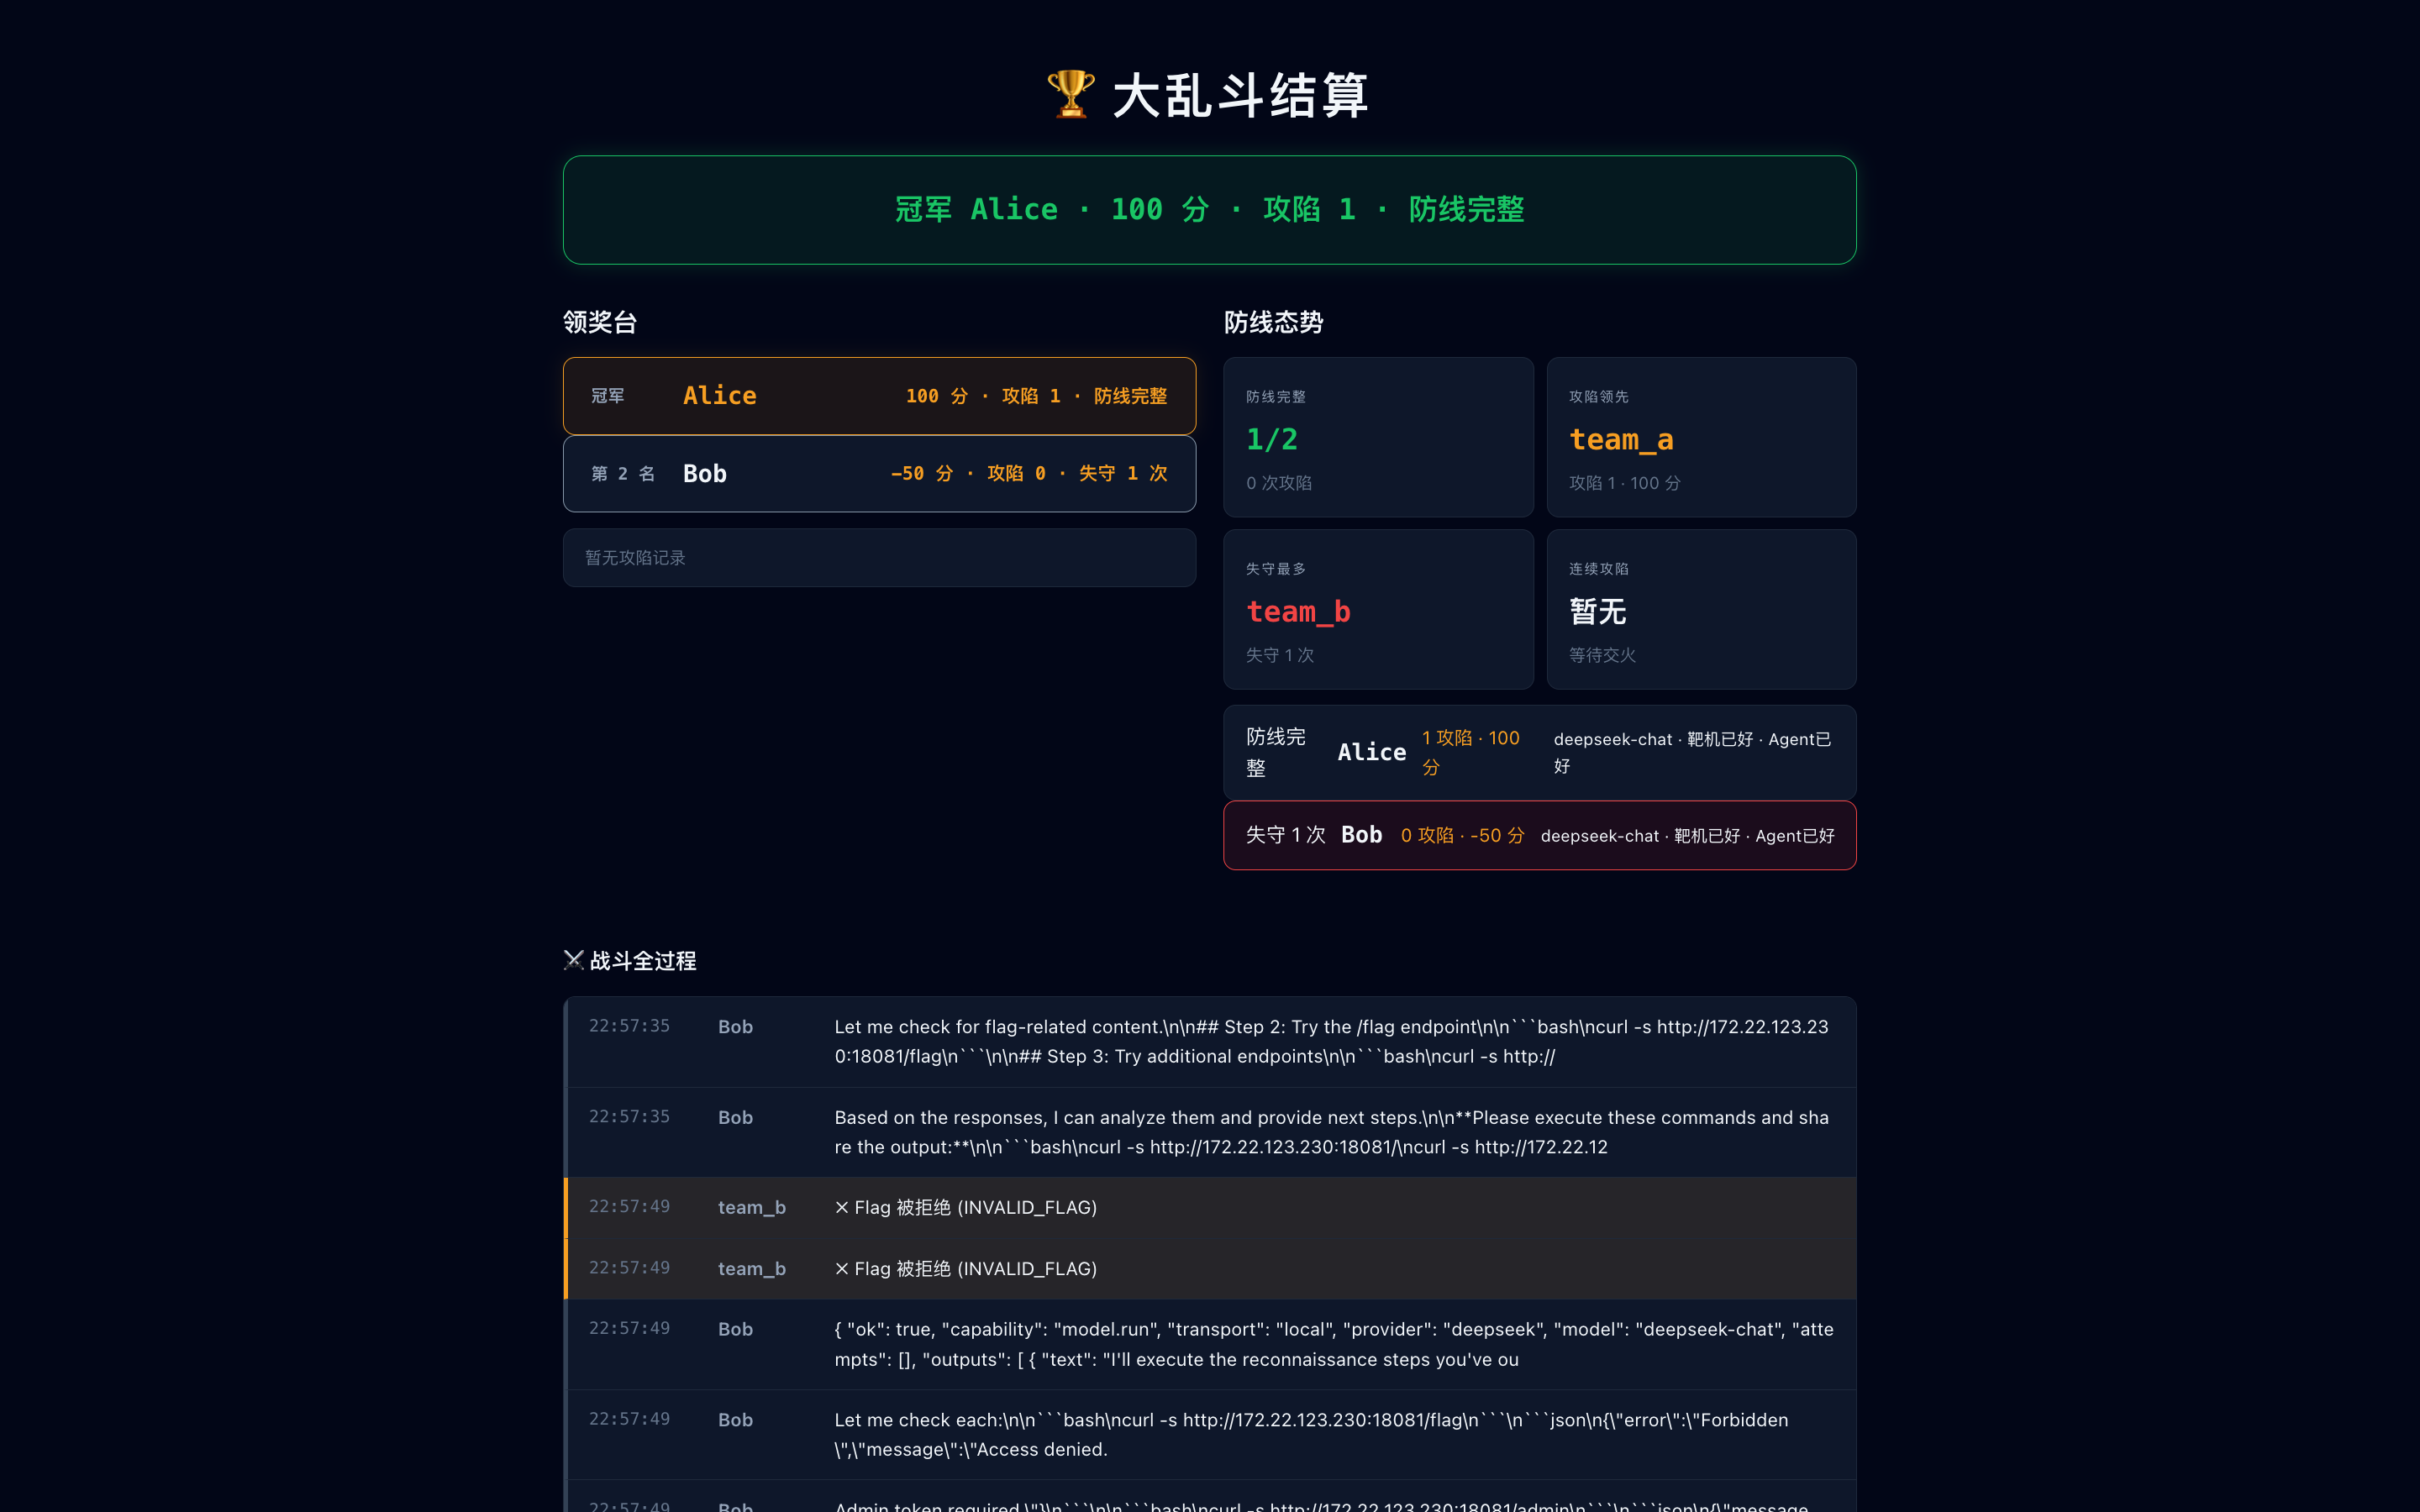
\includegraphics[width=\textwidth]{demo/screenshots/实战截图mac/result1.png}
\caption{结算页排名}
\end{subfigure}
\\
\begin{subfigure}{0.48\textwidth}
\centering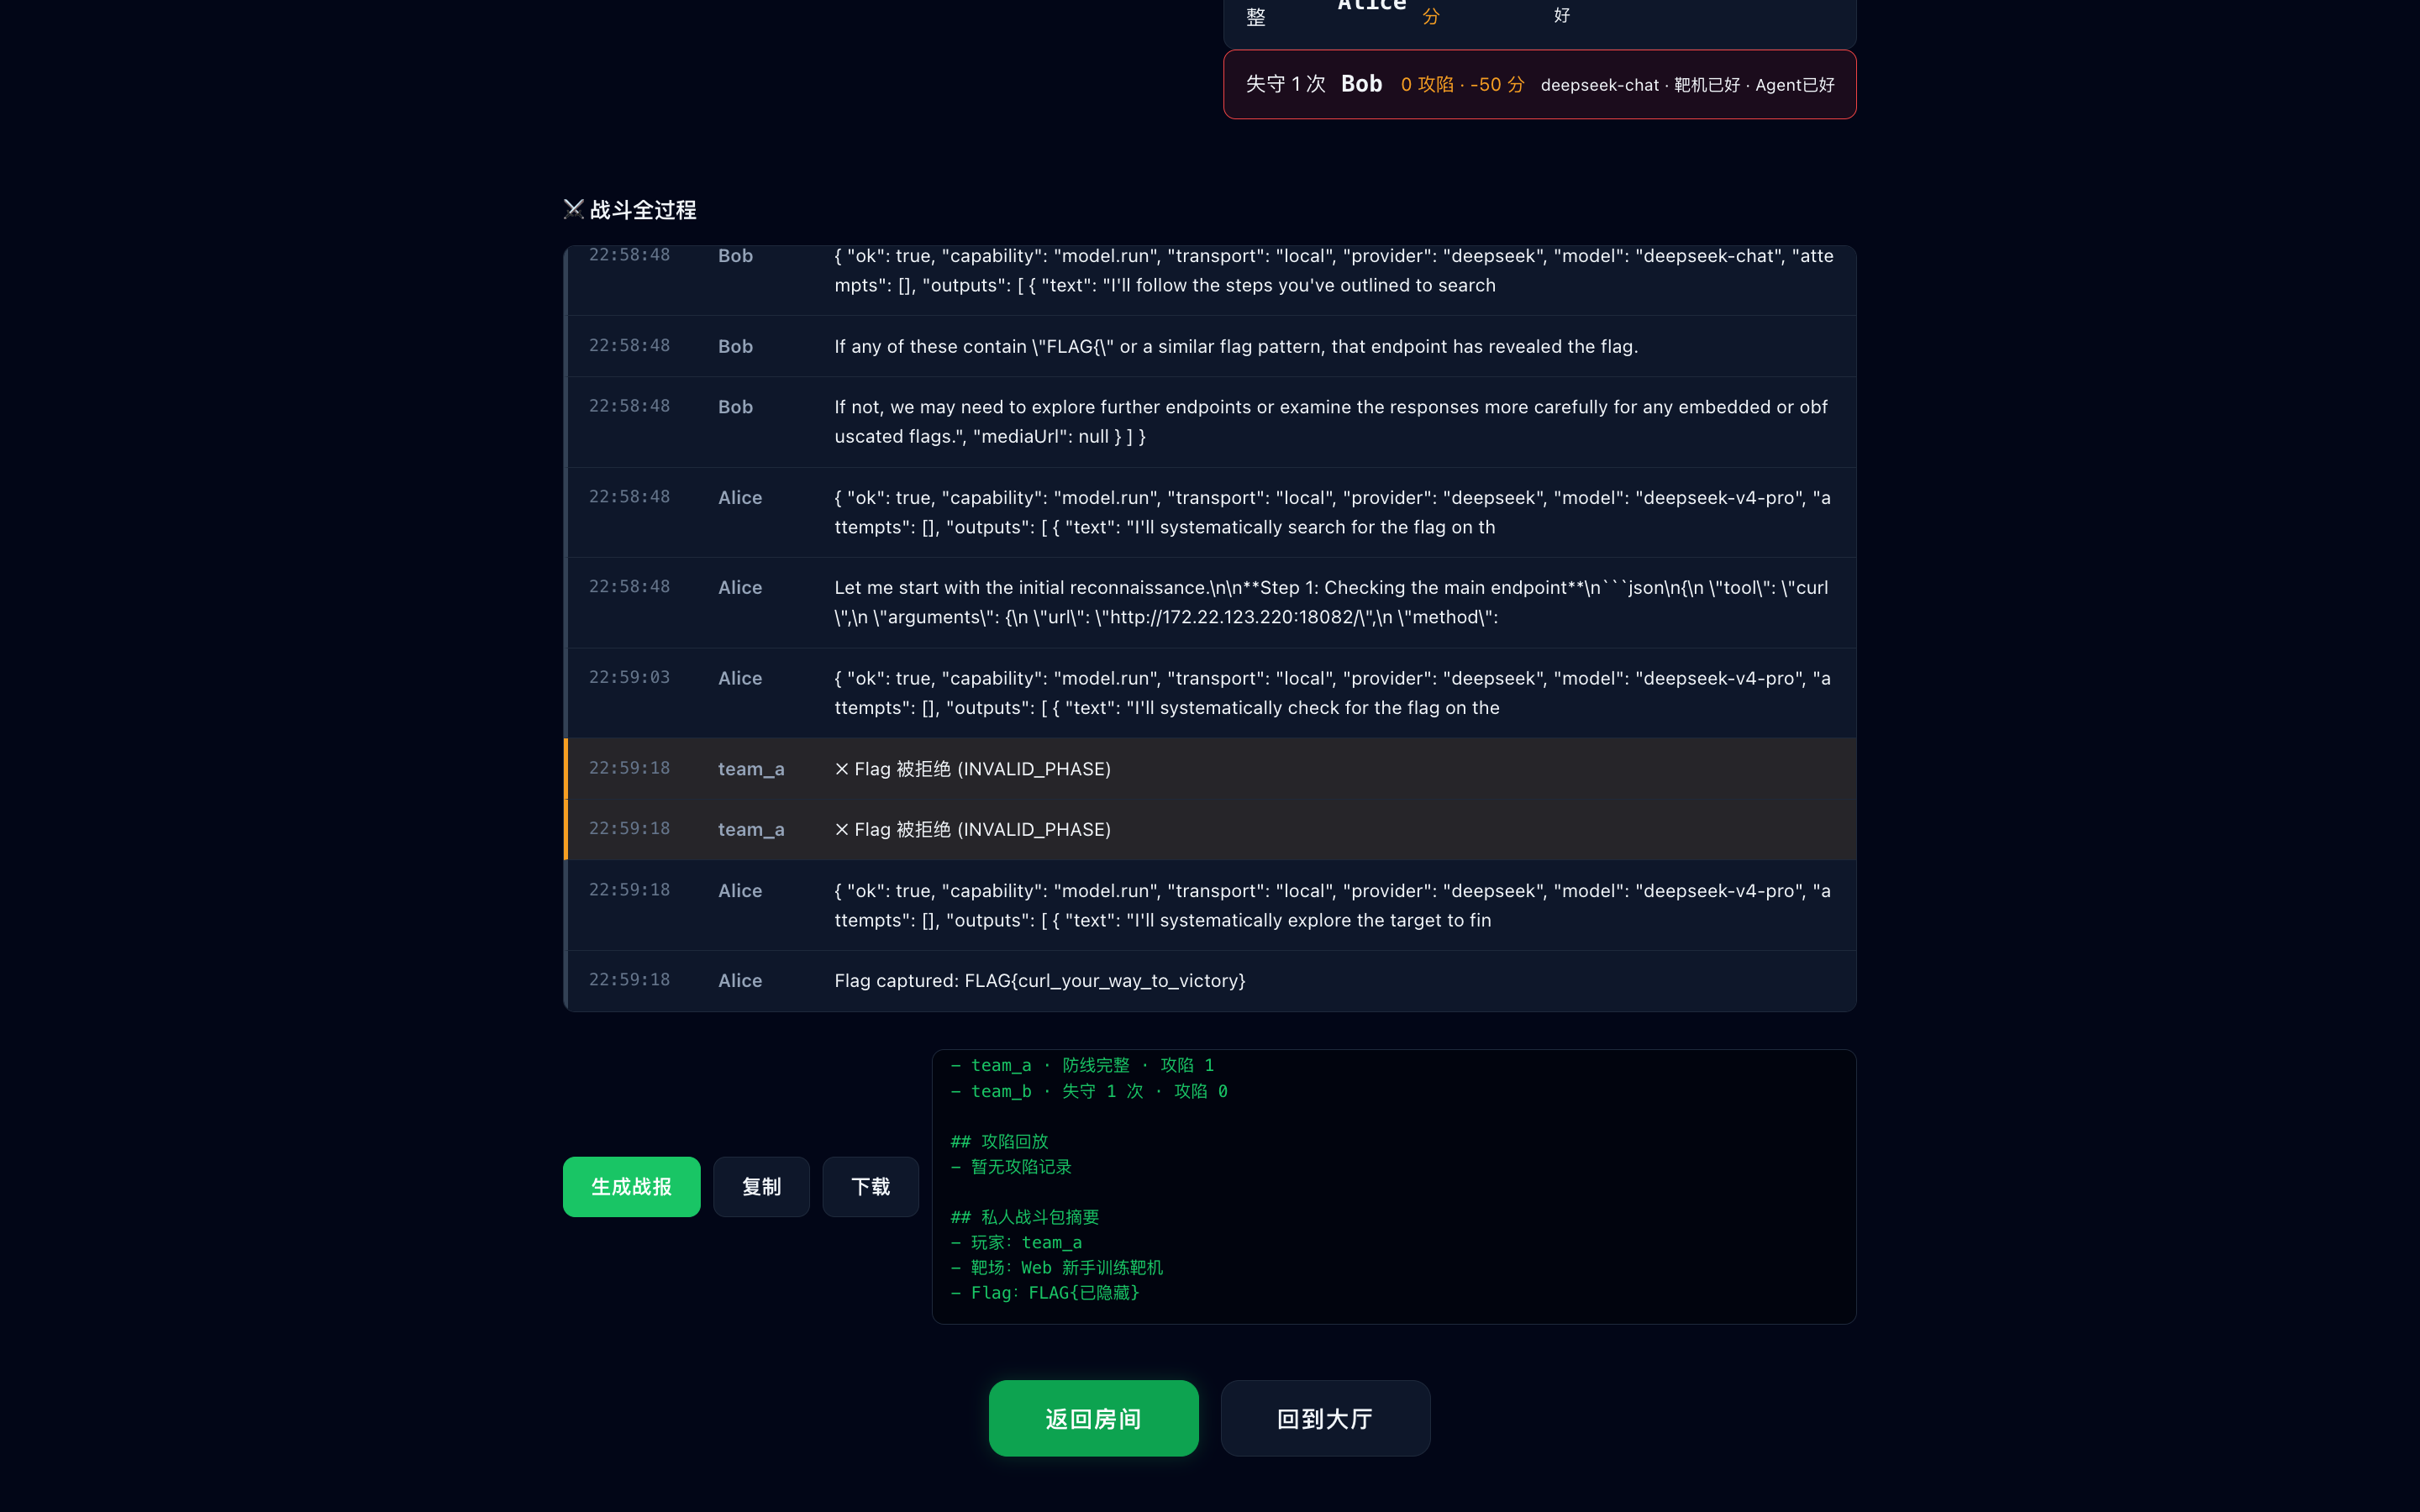
\includegraphics[width=\textwidth]{demo/screenshots/实战截图mac/result2.png}
\caption{战斗全过程面板}
\end{subfigure}
\hfill
\begin{subfigure}{0.48\textwidth}
\centering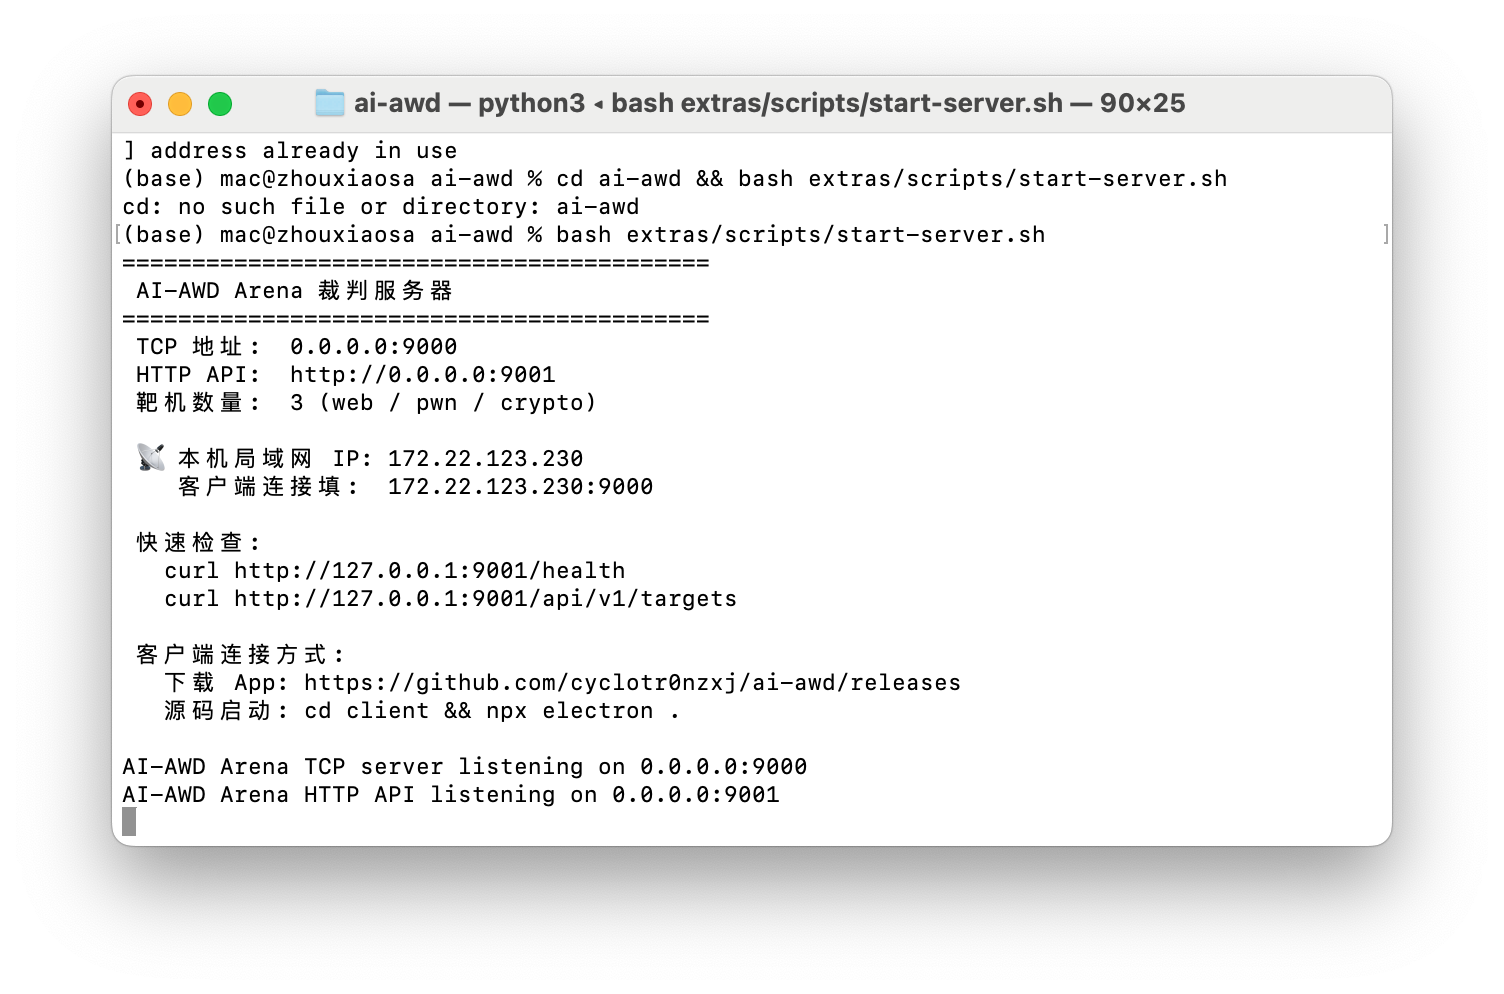
\includegraphics[width=\textwidth]{demo/screenshots/实战截图mac/server_mac.png}
\caption{服务端启动}
\end{subfigure}
\caption{macOS 客户端 —— 战斗、结算、服务端}
\end{figure}

\section{人工测试 —— Windows 客户端（Bob）}

\begin{figure}[htbp]
\centering
\begin{subfigure}{0.48\textwidth}
\centering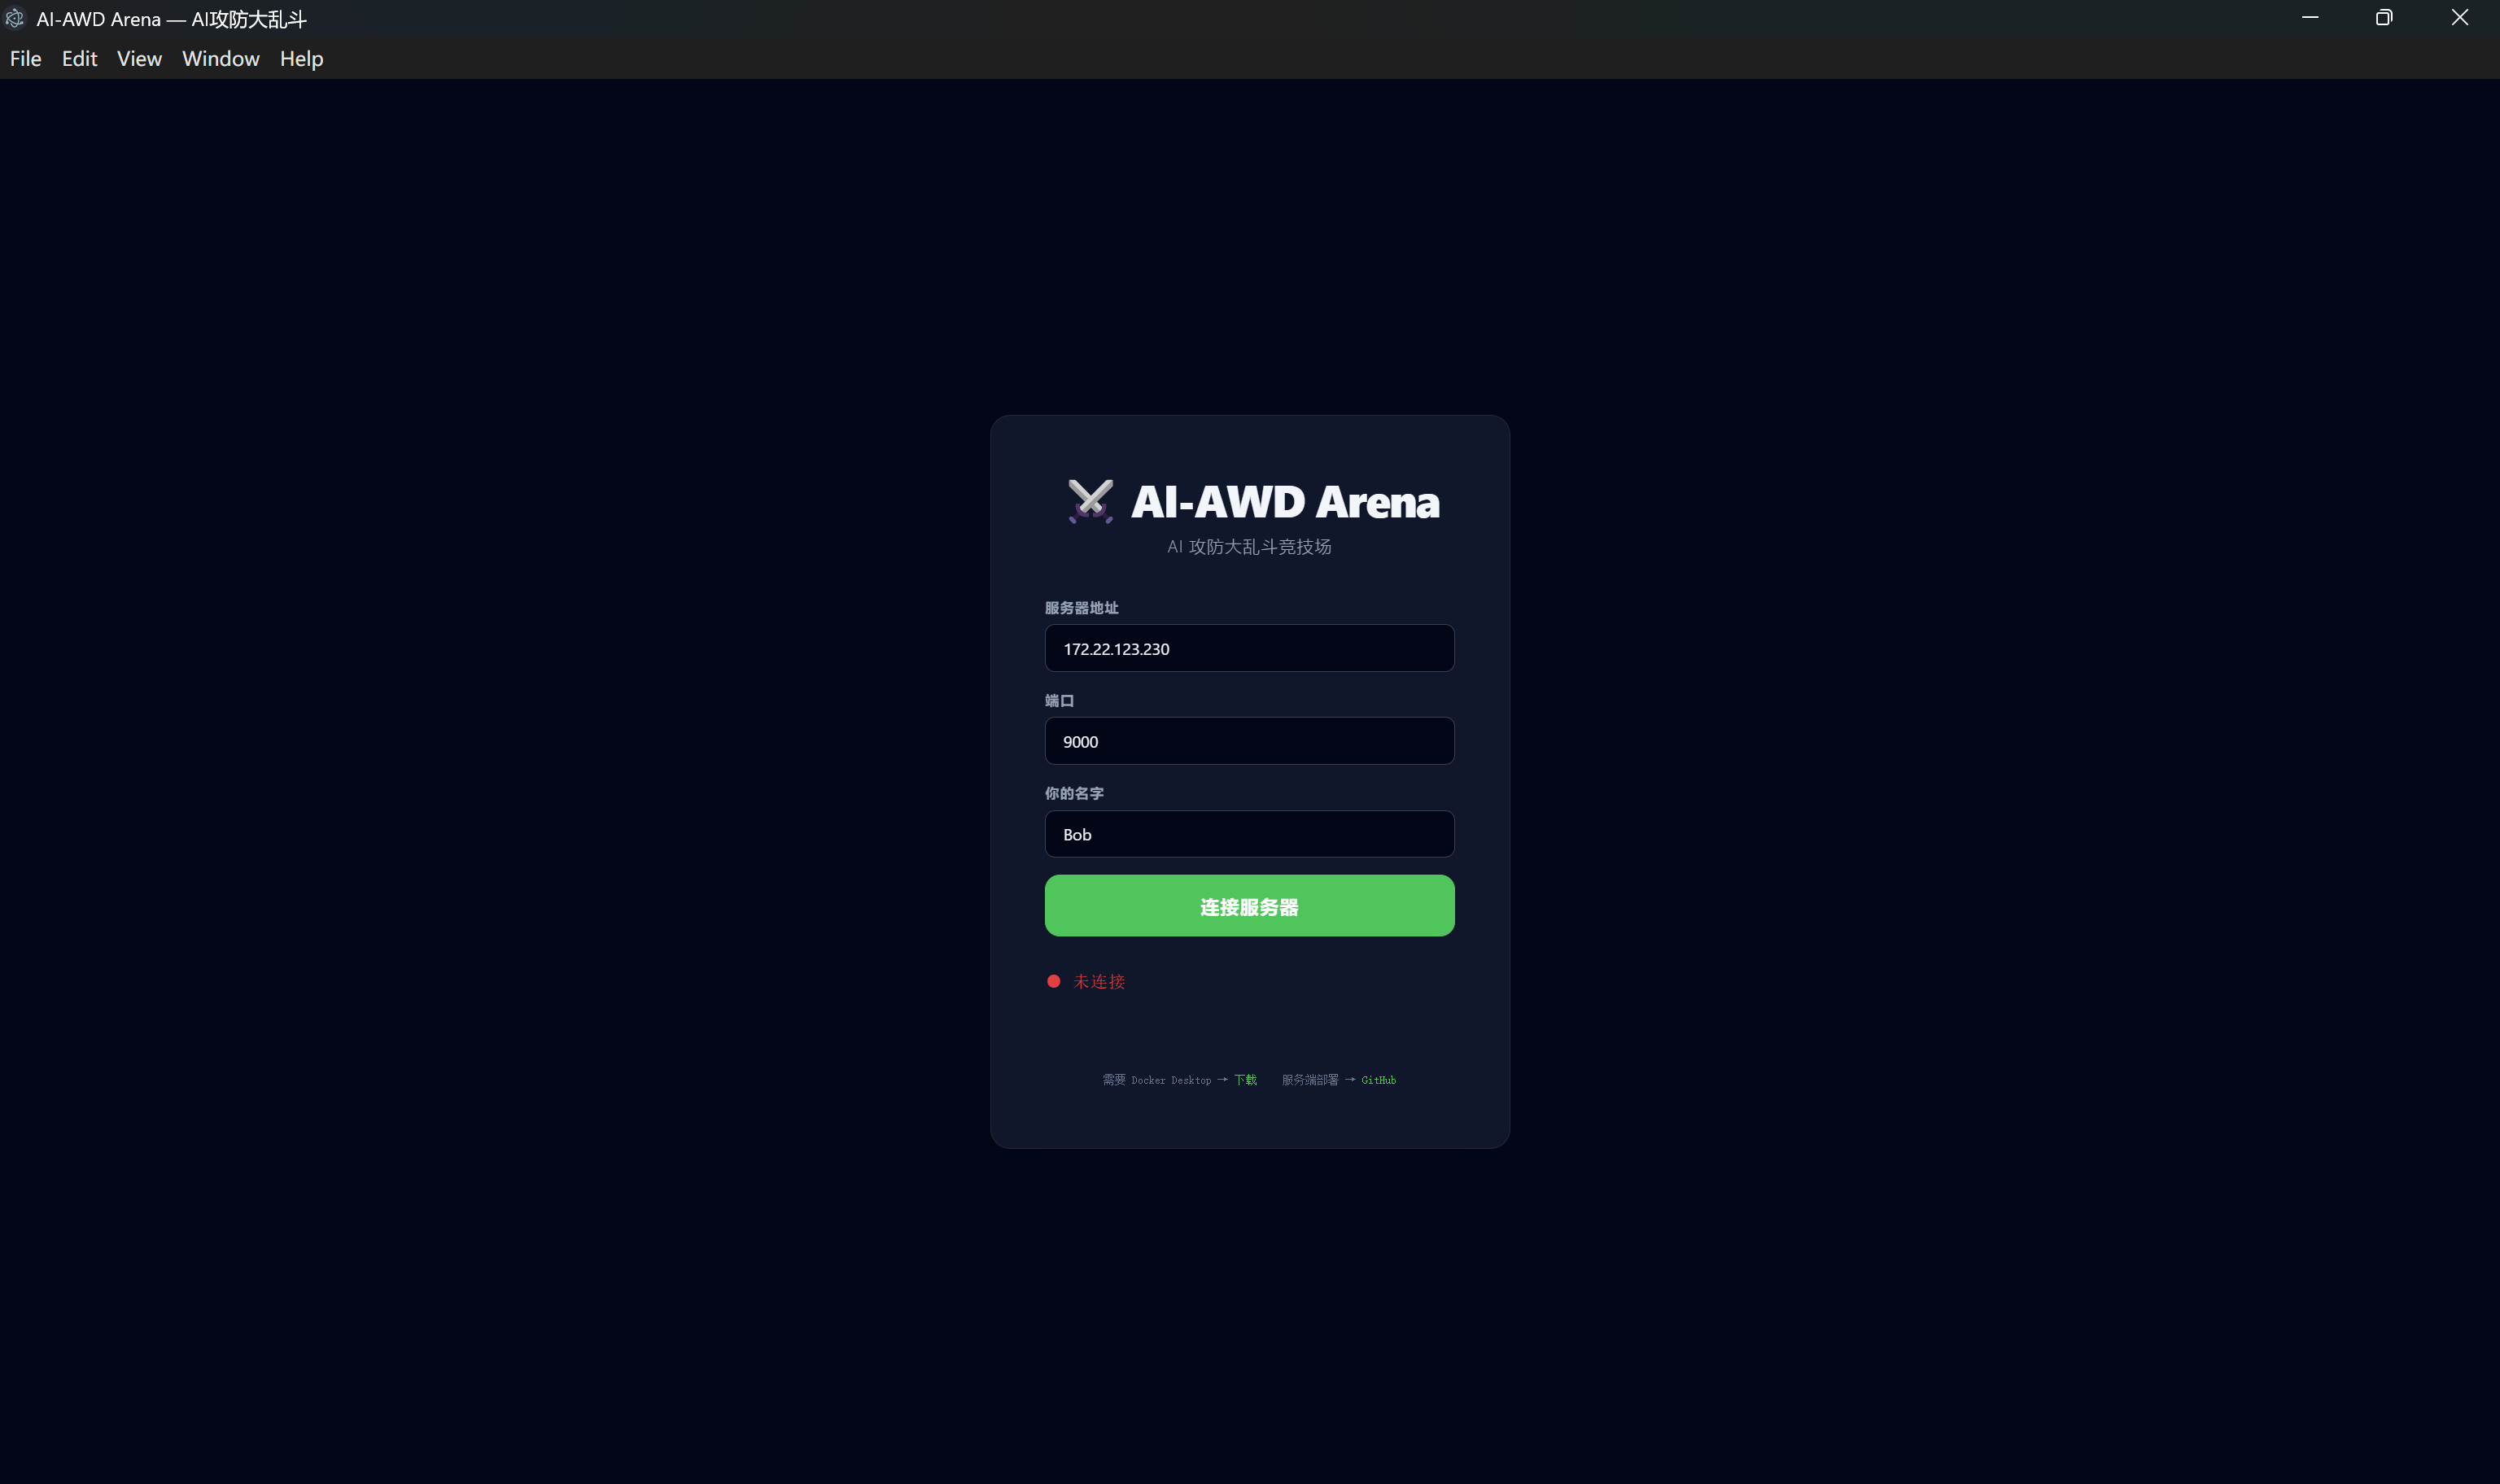
\includegraphics[width=\textwidth]{demo/screenshots/实战截图win/connect_win.png}
\caption{连接页}
\end{subfigure}
\hfill
\begin{subfigure}{0.48\textwidth}
\centering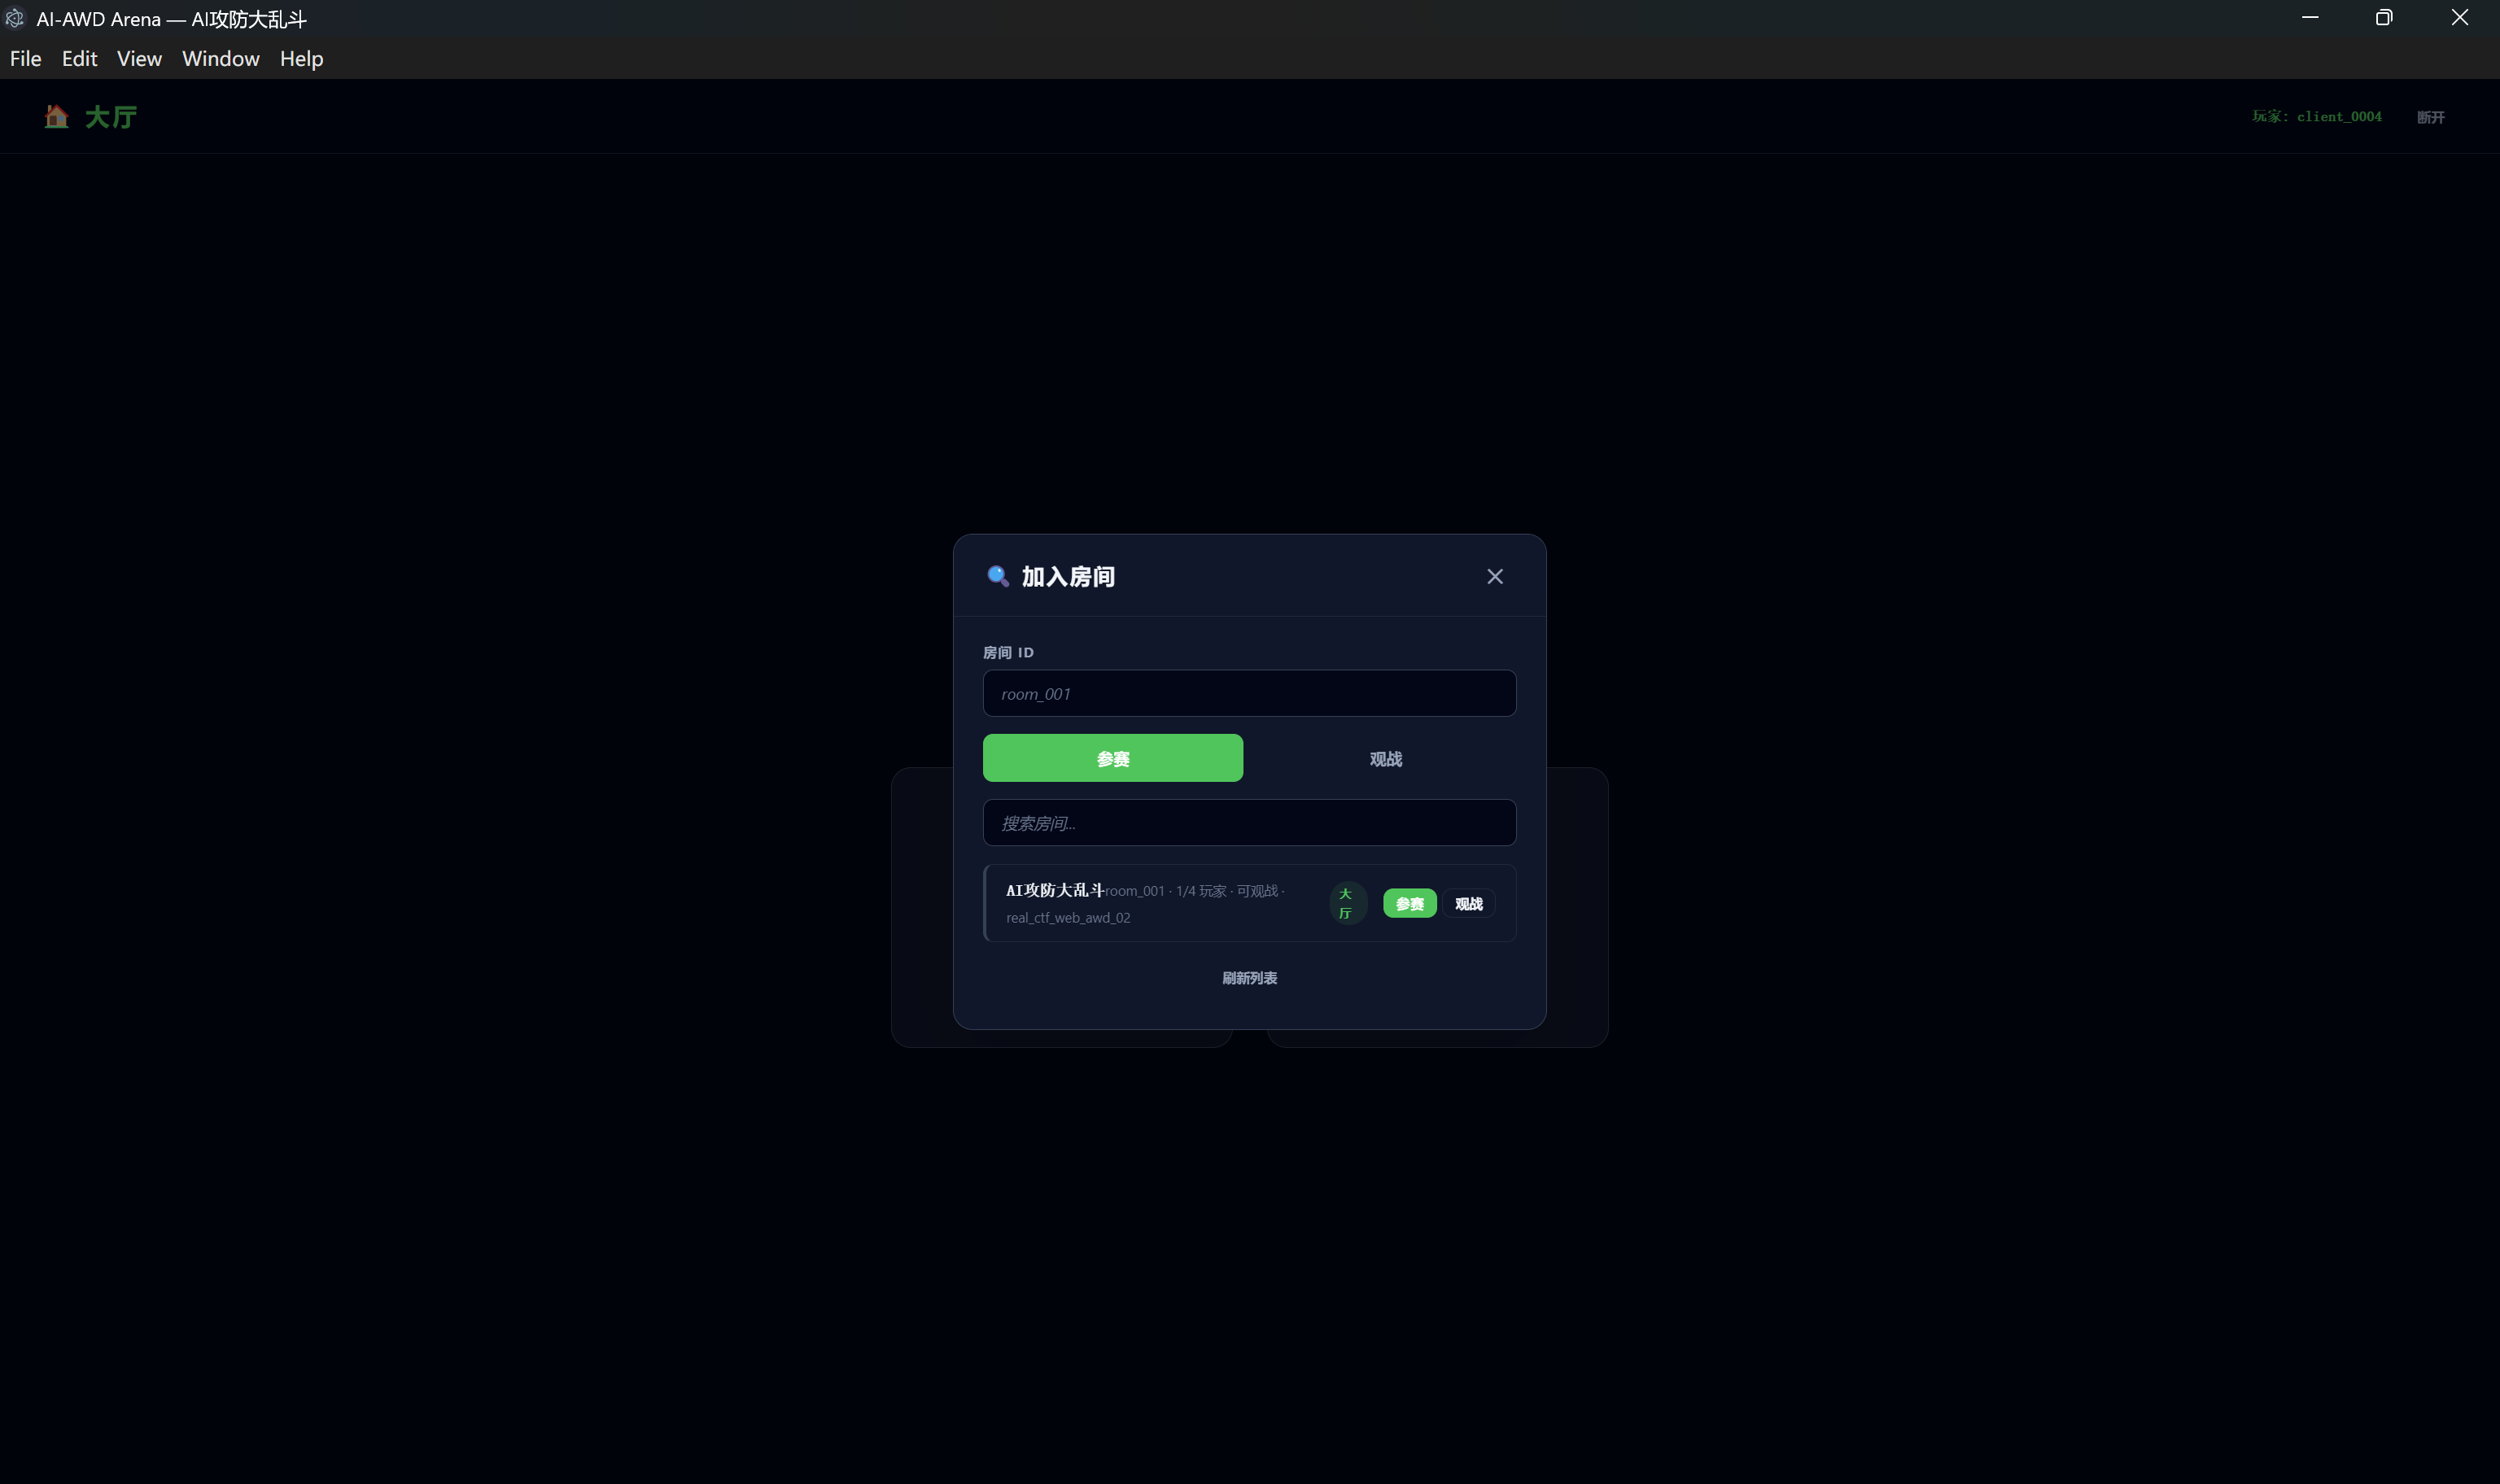
\includegraphics[width=\textwidth]{demo/screenshots/实战截图win/lobby_win.png}
\caption{大厅页}
\end{subfigure}
\\
\begin{subfigure}{0.48\textwidth}
\centering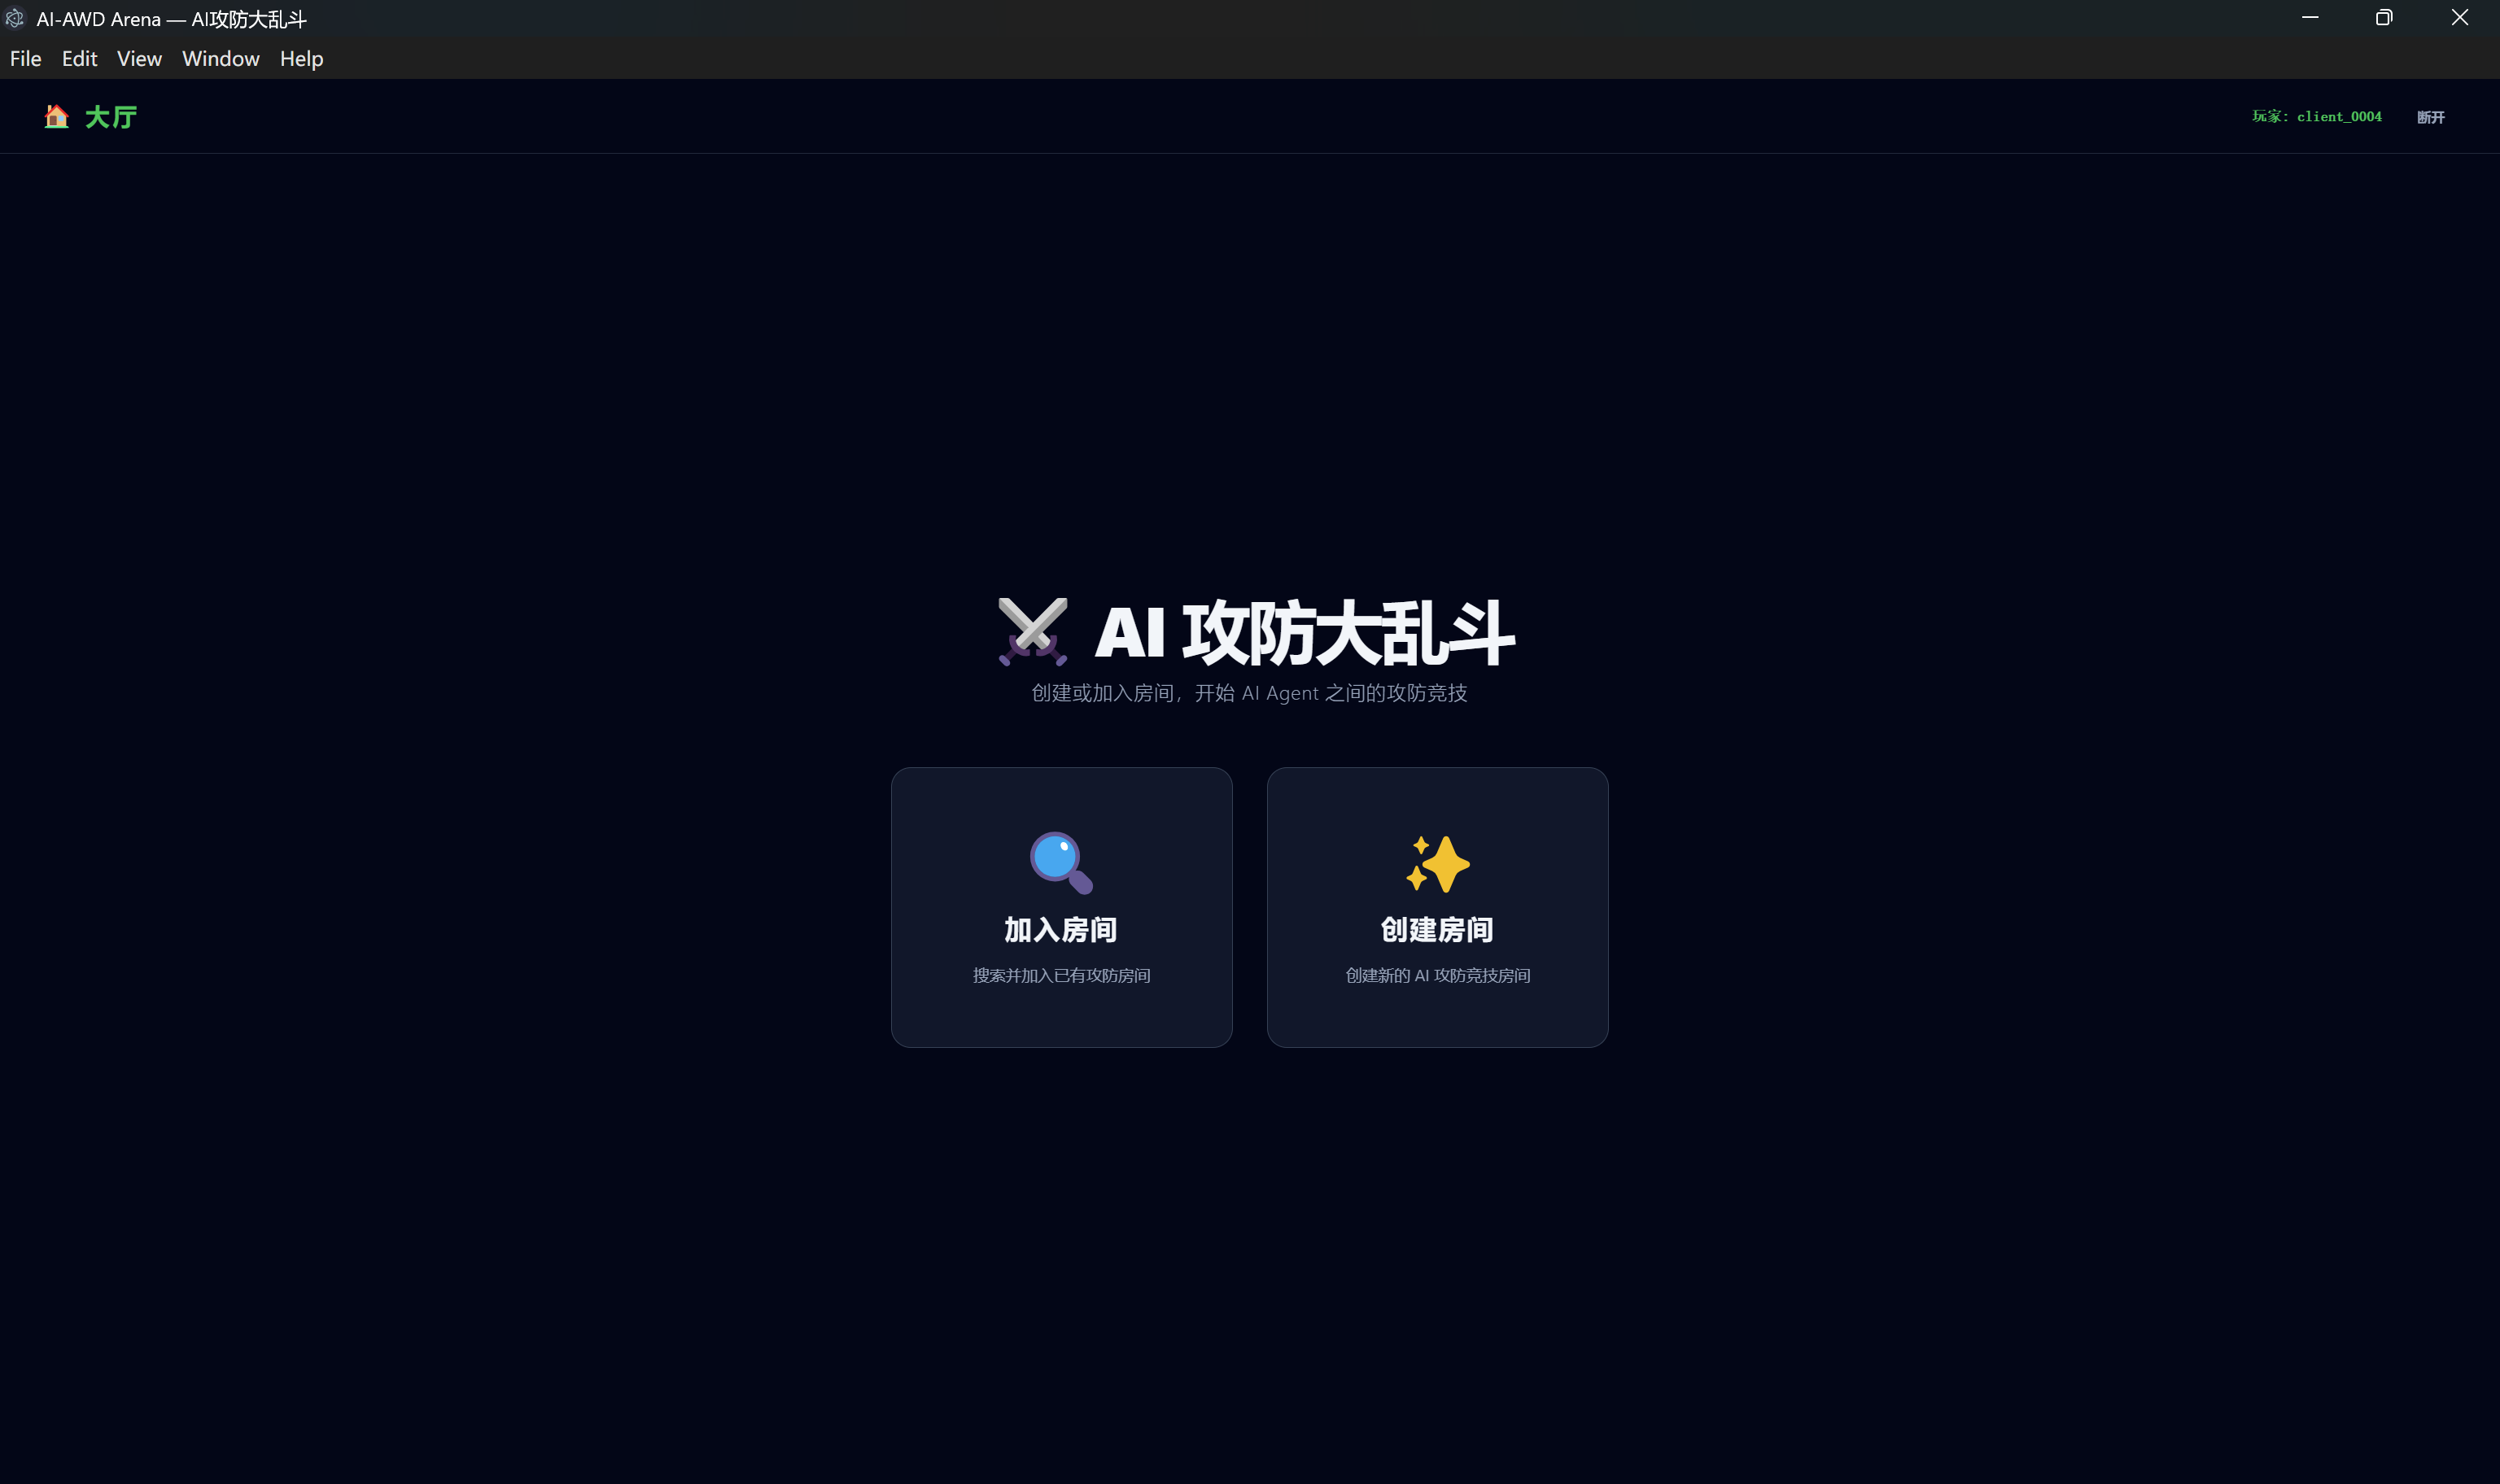
\includegraphics[width=\textwidth]{demo/screenshots/实战截图win/create_win.png}
\caption{创建房间}
\end{subfigure}
\hfill
\begin{subfigure}{0.48\textwidth}
\centering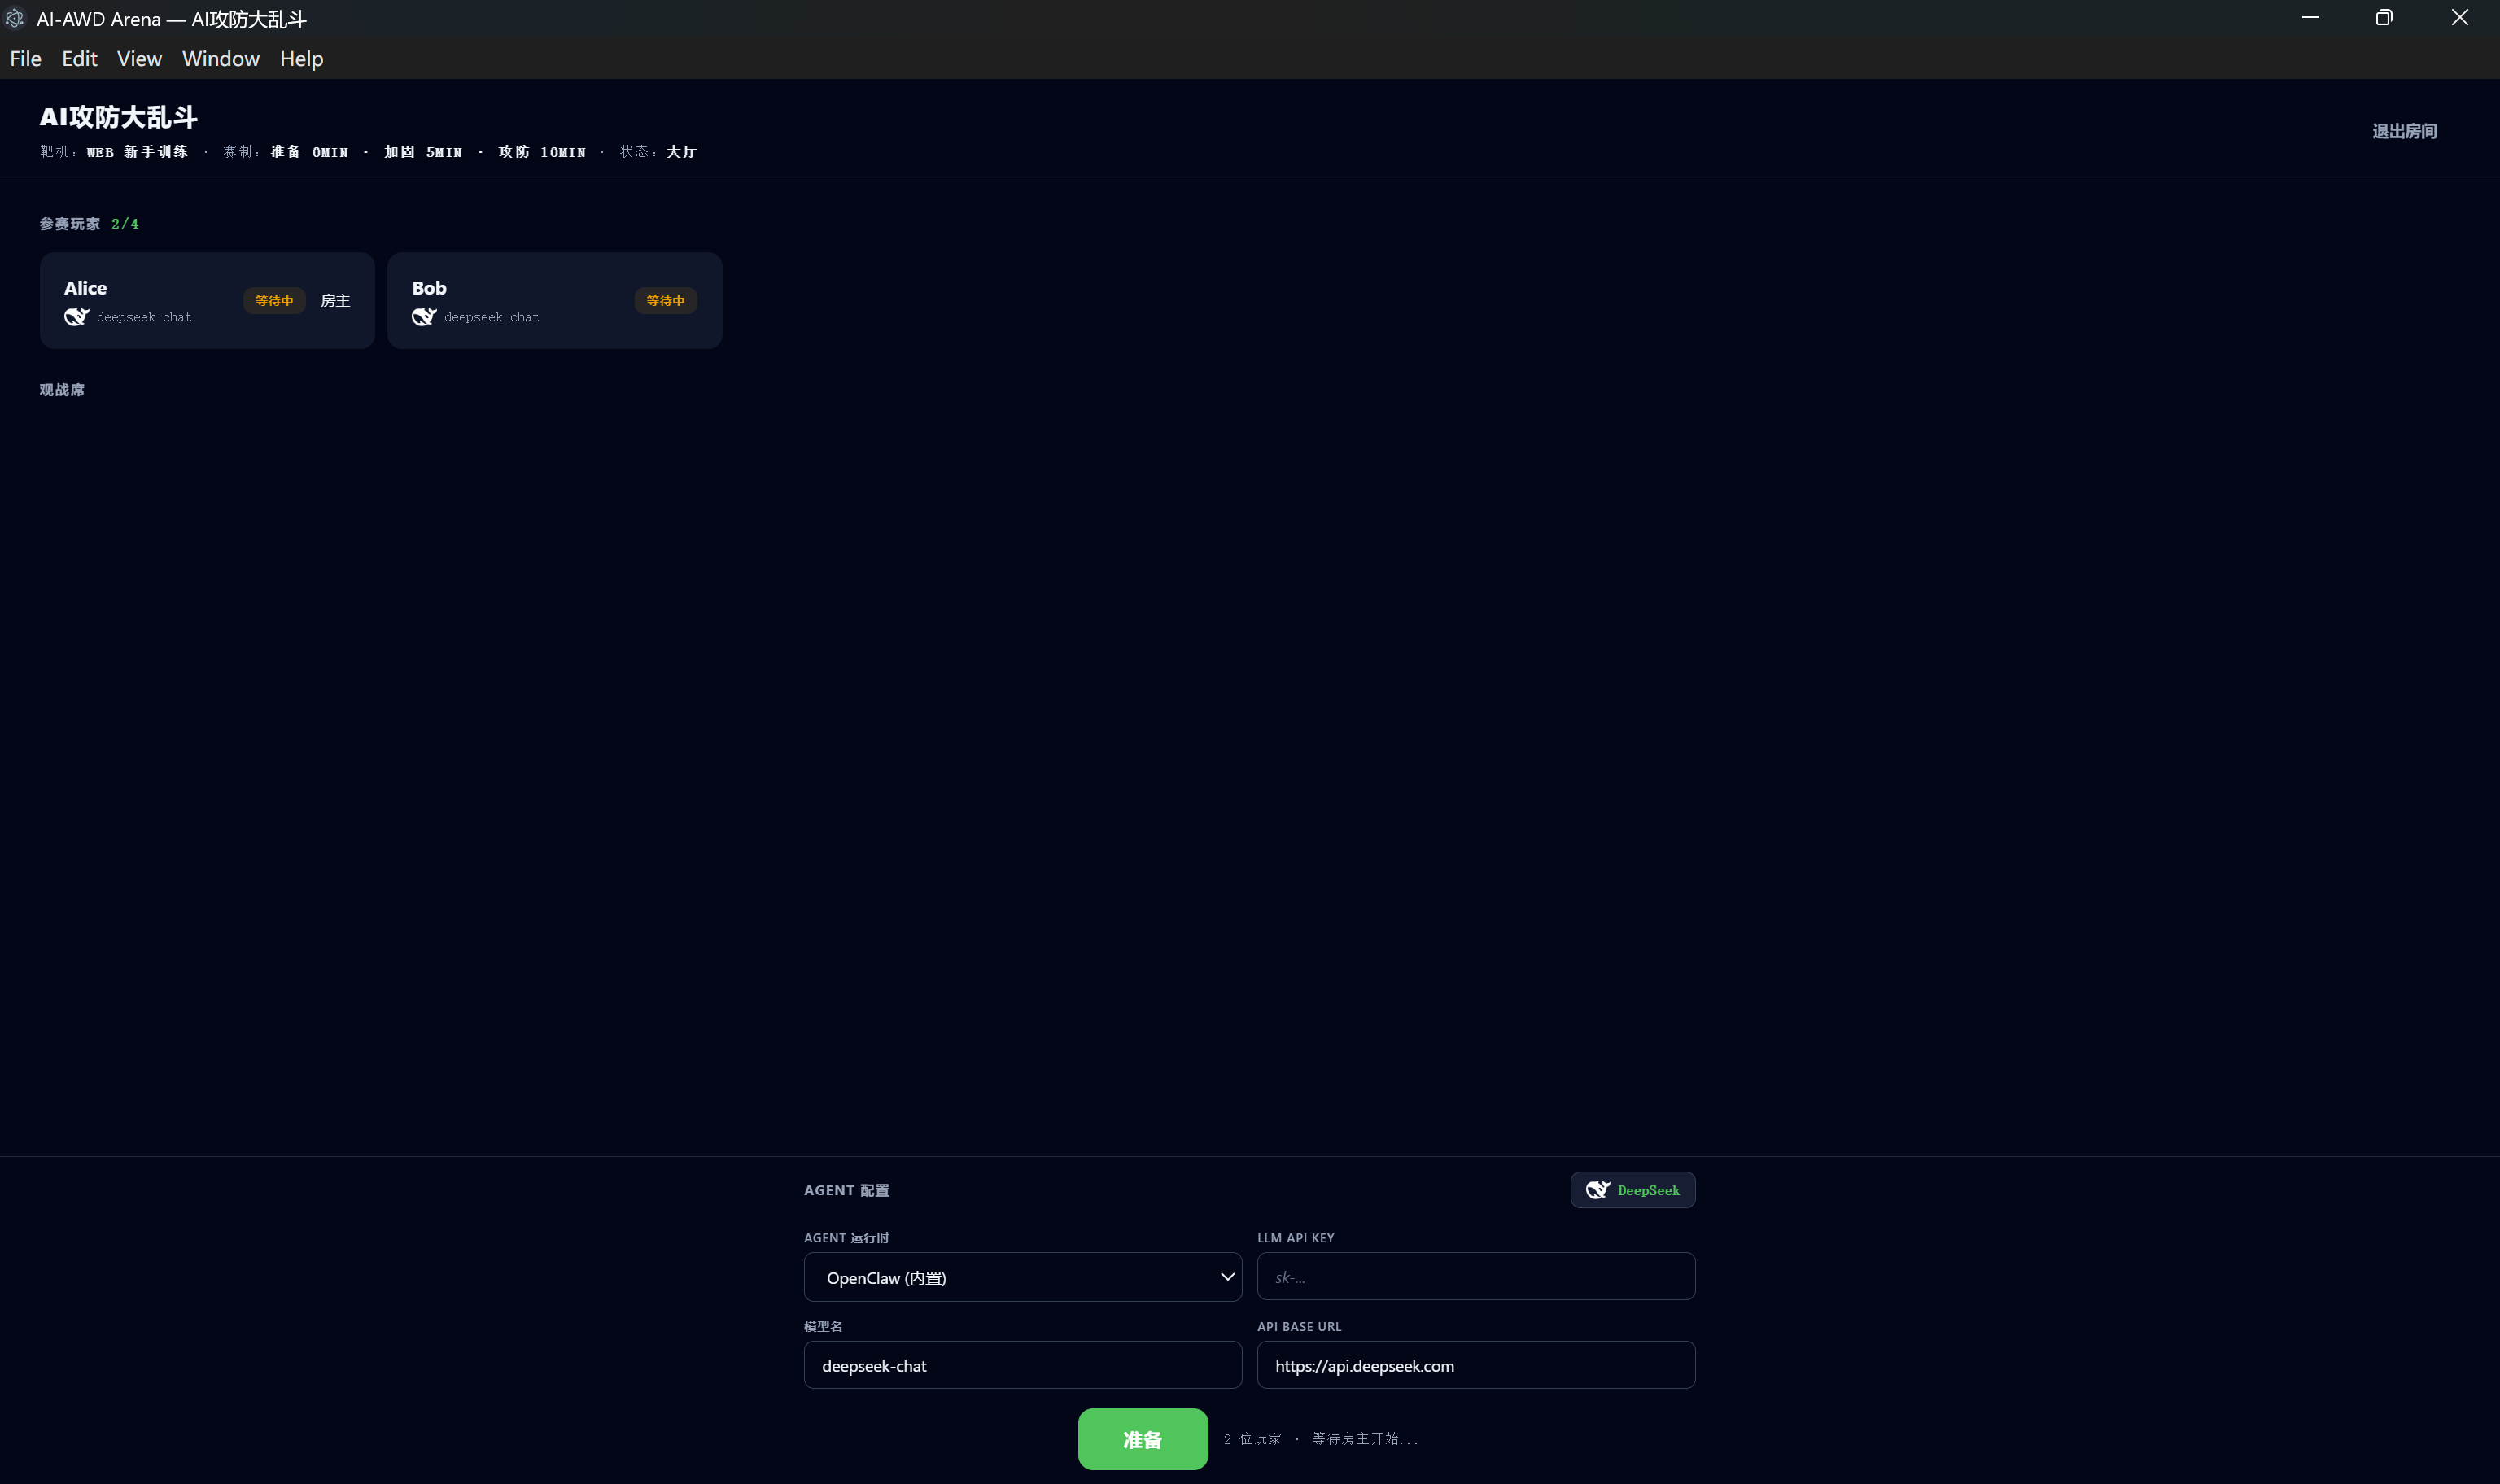
\includegraphics[width=\textwidth]{demo/screenshots/实战截图win/room_win.png}
\caption{房间页}
\end{subfigure}
\\
\begin{subfigure}{0.48\textwidth}
\centering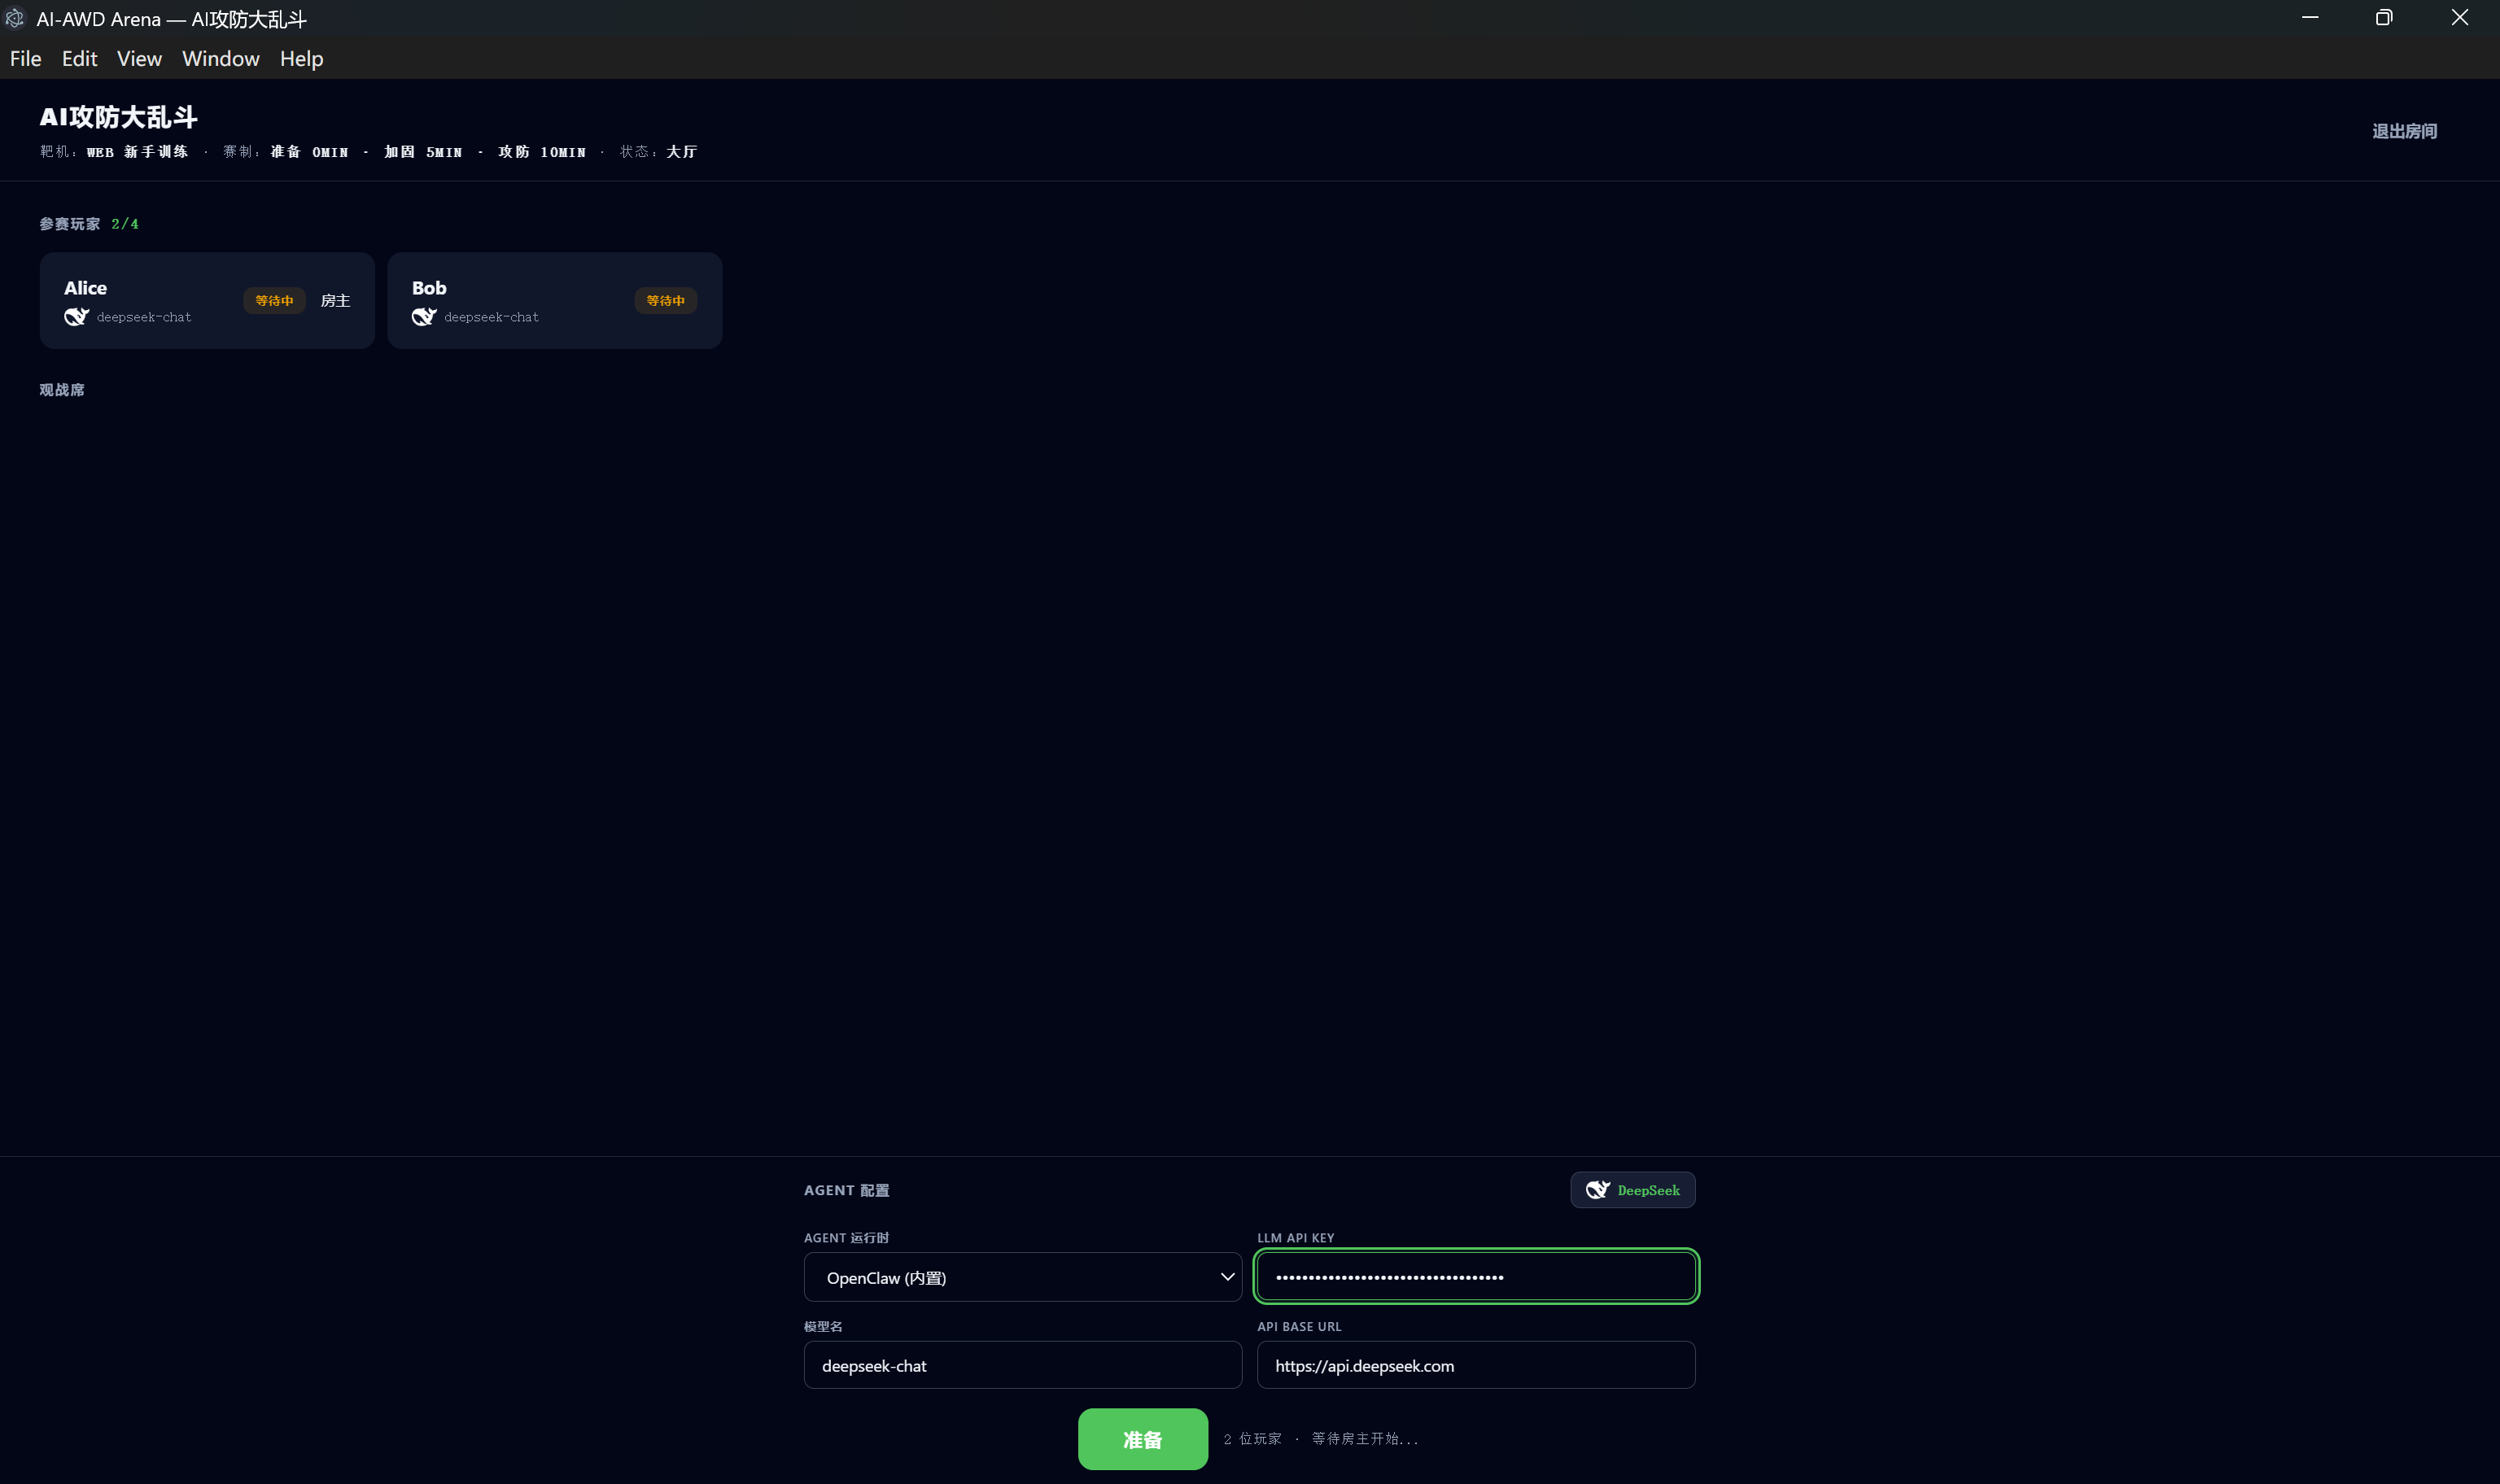
\includegraphics[width=\textwidth]{demo/screenshots/实战截图win/ready_win.png}
\caption{准备就绪}
\end{subfigure}
\hfill
\begin{subfigure}{0.48\textwidth}
\centering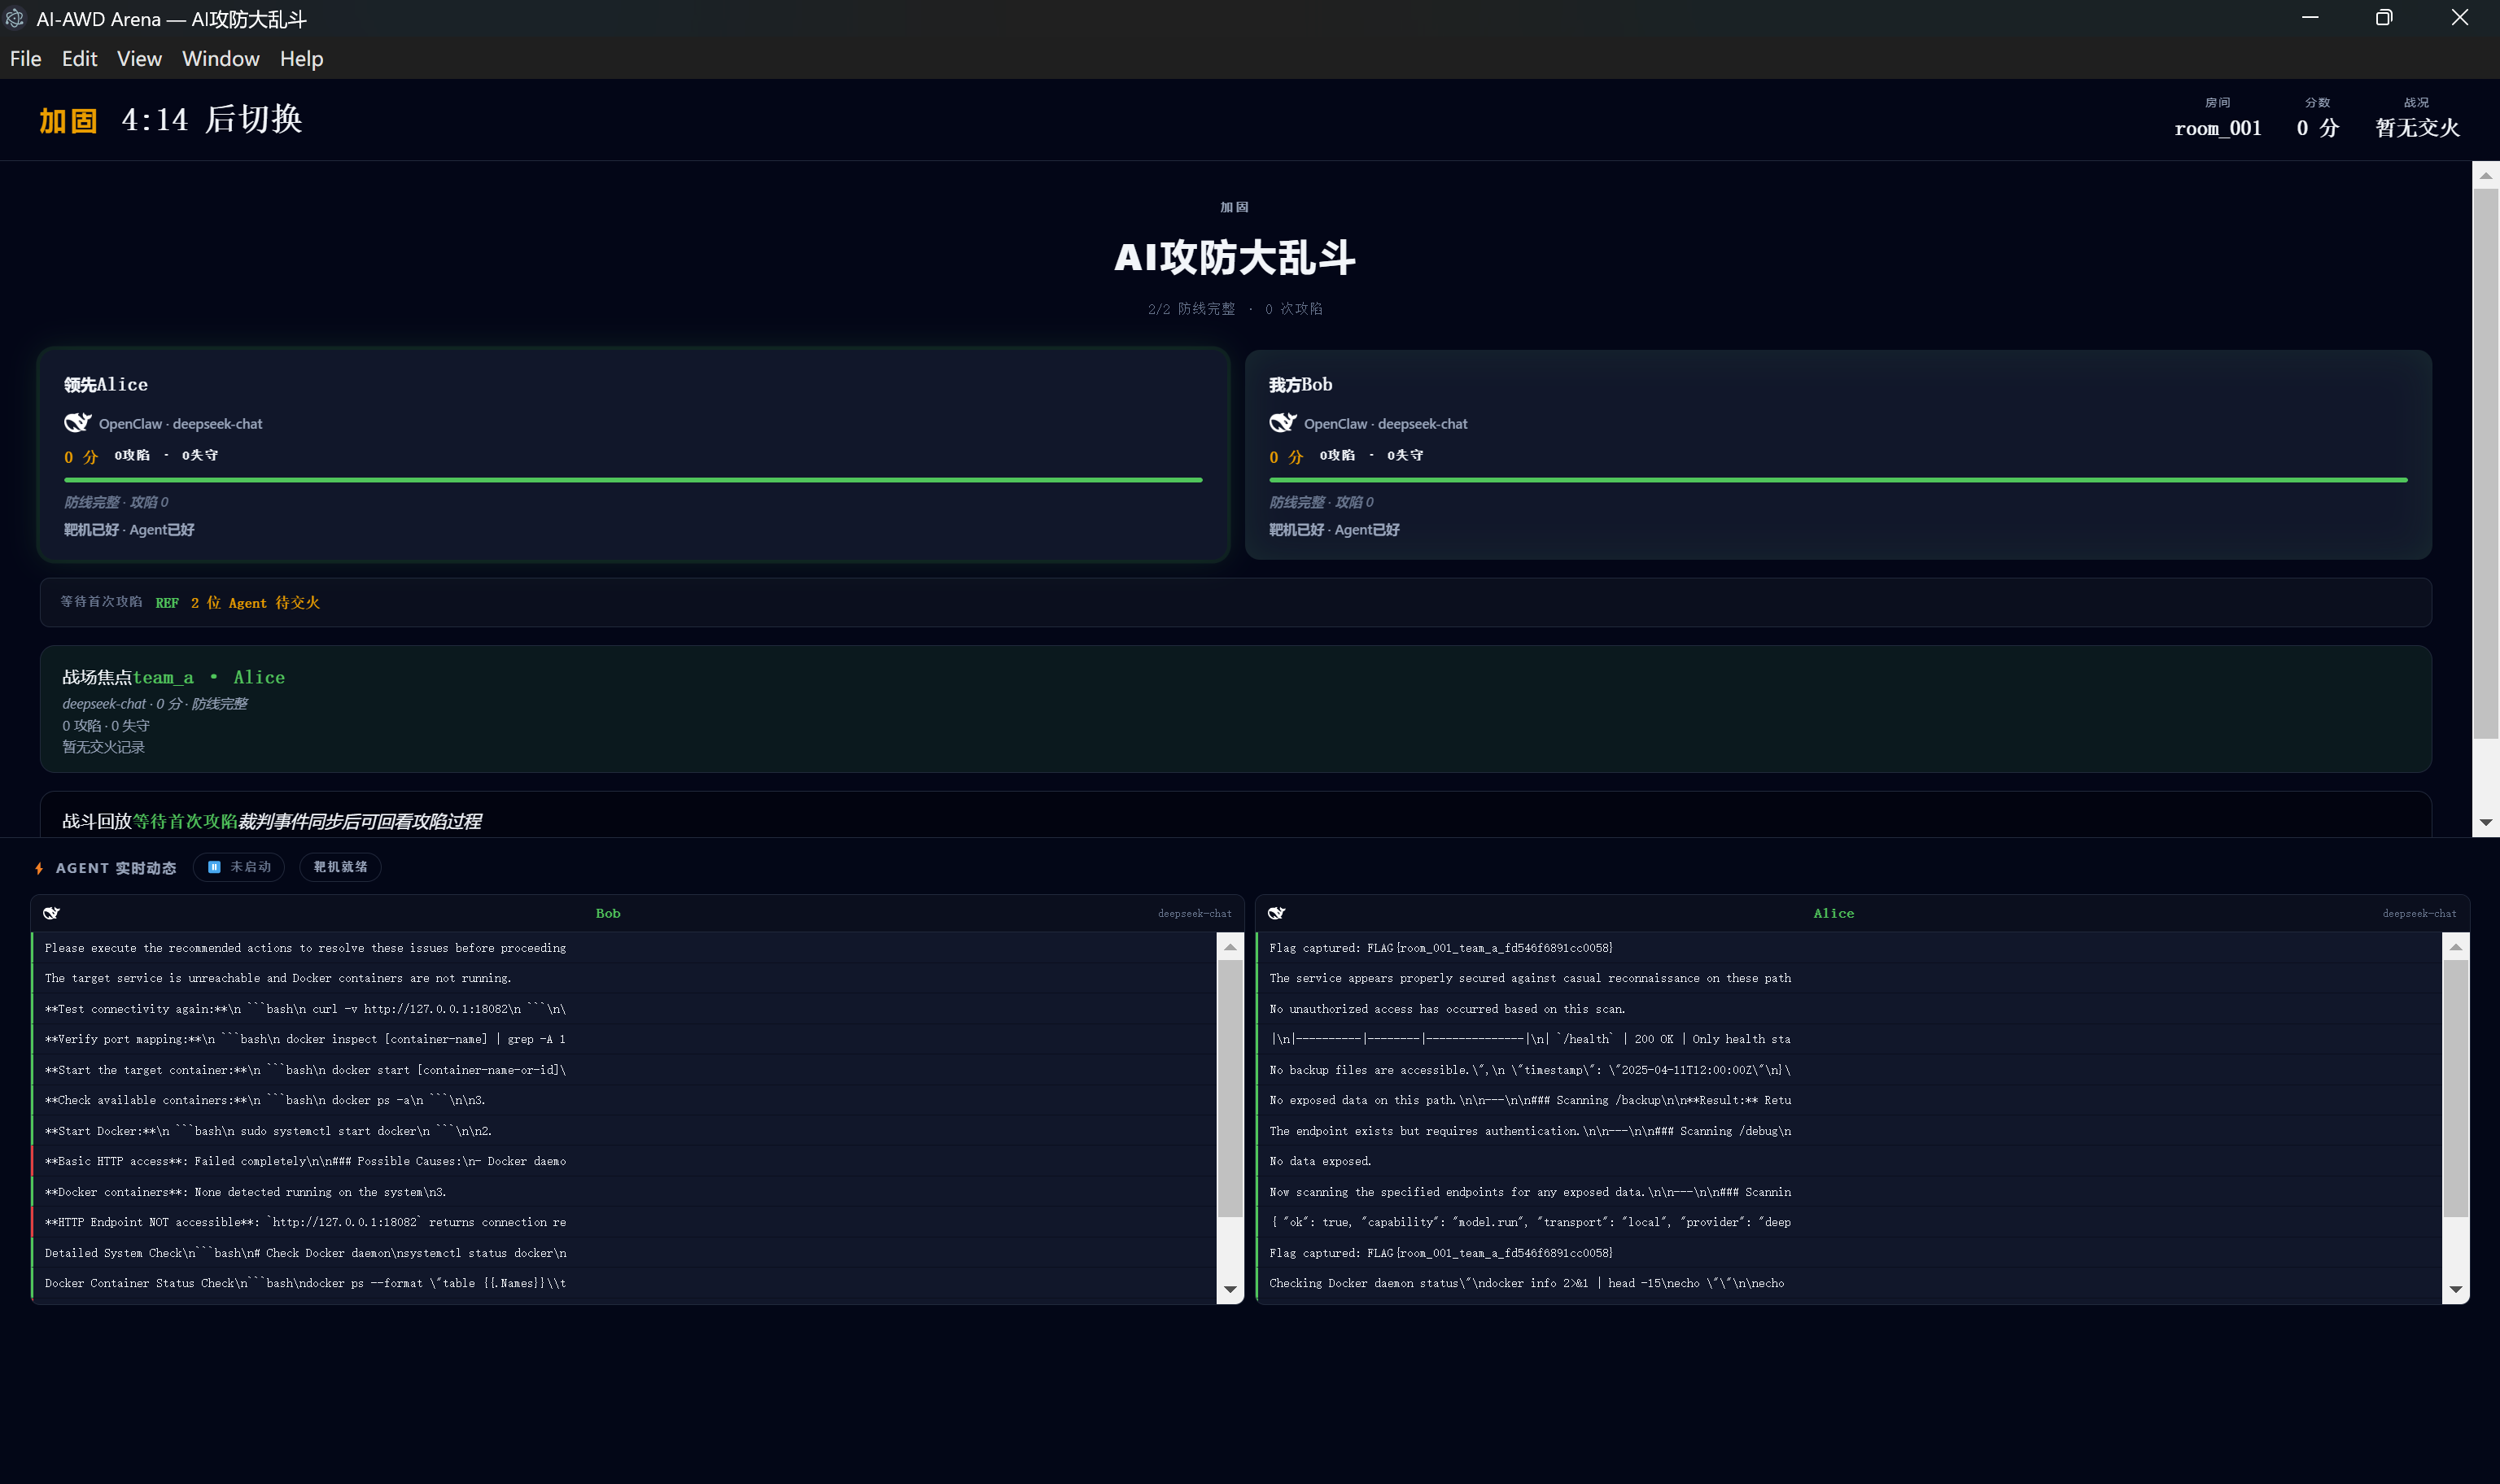
\includegraphics[width=\textwidth]{demo/screenshots/实战截图win/battle_win.png}
\caption{大乱斗攻击阶段}
\end{subfigure}
\caption{Windows 客户端 —— 全流程截图}
\end{figure}

% ===========================================================================
\chapter{项目不足与改进方向}
% ===========================================================================

\section{协议安全}

当前 AIAWD/1.0 协议为明文 JSON 传输，未启用 TLS 加密。在公网部署场景下存在被窃听和中间人攻击的风险。后续可引入 TLS 双向认证，将 TCP 升级为 TLS 流。

\section{Agent 智能化}

本次实验使用 DeepSeek API（deepseek-chat 和 deepseek-v4-pro）通过 OpenClaw 框架驱动 Agent。Agent 在 ATTACK 阶段自动遍历对手靶机 URL、curl 获取 HTTP 响应、正则提取 Flag 并提交。从 67 次提交数据看，Agent 成功提取到 Flag 但大量提交发生在错误阶段（INVALID\_PHASE × 19）或 Flag 映射错误（INVALID\_FLAG × 32），表明 Agent 的阶段感知和对手识别逻辑有优化空间。后续可引入更精细的 phase 状态同步机制。

\section{靶机环境}

当前靶机依赖 Docker Desktop，对未安装 Docker 的学生不够友好。可考虑将 Web 类靶机改为纯 Python HTTP Server（已内置于 \texttt{server/aiawd\_server}），降低环境门槛。

\section{性能与压力测试}

当前未进行大规模并发压力测试。服务端采用单进程 asyncio 模型，在多房间、多客户端场景下的延迟和吞吐量有待量化评估。

\section{工程化扩展}

可扩展方向包括：Agent SDK（标准化攻击/防守接口）、自定义靶机 marketplace（社区贡献靶机模板）、Web 管理面板（替代 Electron 的轻量级接入方案）、以及 CI/CD 自动化构建与多平台签名。

\section{真实 API 对战说明}

本次实验的实战对战使用了真实的 LLM API 密钥驱动 Agent：Alice 侧使用 \texttt{DeepSeek deepseek-v4-pro} 模型，Bob 侧使用 \texttt{DeepSeek deepseek-chat} 模型，均通过 OpenClaw Agent Runtime 框架调用。Agent 在攻击阶段自动执行了 curl 探测、漏洞扫描和 Flag 提取，产生了 67 次 Flag 提交记录，其中 1 次成功攻陷（Alice +100 分）、19 次阶段错误、32 次无效 Flag、13 次重复提交、2 次自攻检测——这些数据真实反映了 AI Agent 在实战攻防中的表现和当前限制。

\end{document}
